%%%%%%%%%%%%%%%%%%%%%%%%%%%%%%%%%%%%%%%%%
% Masters/Doctoral Thesis 
% LaTeX Template
% Version 2.5 (27/8/17)
%
% This template was downloaded from:
% http://www.LaTeXTemplates.com
%
% Version 2.x major modifications by:
% Vel (vel@latextemplates.com)
%
% This template is based on a template by:
% Steve Gunn (http://users.ecs.soton.ac.uk/srg/softwaretools/document/templates/)
% Sunil Patel (http://www.sunilpatel.co.uk/thesis-template/)
%
% Template license:
% CC BY-NC-SA 3.0 (http://creativecommons.org/licenses/by-nc-sa/3.0/)
%
%%%%%%%%%%%%%%%%%%%%%%%%%%%%%%%%%%%%%%%%%

%----------------------------------------------------------------------------------------
%   PACKAGES AND OTHER DOCUMENT CONFIGURATIONS
%----------------------------------------------------------------------------------------

\documentclass[
11pt, % The default document font size, options: 10pt, 11pt, 12pt
%oneside, % Two side (alternating margins) for binding by default, uncomment to switch to one side
english, % ngerman for German
singlespacing, % Single line spacing, alternatives: onehalfspacing or doublespacing
%draft, % Uncomment to enable draft mode (no pictures, no links, overfull hboxes indicated)
%nolistspacing, % If the document is onehalfspacing or doublespacing, uncomment this to set spacing in lists to single
%liststotoc, % Uncomment to add the list of figures/tables/etc to the table of contents
%toctotoc, % Uncomment to add the main table of contents to the table of contents
%parskip, % Uncomment to add space between paragraphs
%nohyperref, % Uncomment to not load the hyperref package
headsepline, % Uncomment to get a line under the header
%chapterinoneline, % Uncomment to place the chapter title next to the number on one line
%consistentlayout, % Uncomment to change the layout of the declaration, abstract and acknowledgements pages to match the default layout
]{MastersDoctoralThesis} % The class file specifying the document structure

\usepackage{pdfpages} % enables add pdf pages

%\usepackage{draftwatermark} % DRAFT MARK
%\SetWatermarkLightness{0.8}
%\SetWatermarkScale{1}

\usepackage{comment} % comment large parts of latex using \iffalse \fi

\usepackage{enumitem} % \enumerate with \Alph

\usepackage{siunitx} % for using \ang{30} for 30º

\usepackage[utf8]{inputenc} % Required for inputting international characters
\usepackage[T1]{fontenc} % Output font encoding for international characters

\usepackage{mathpazo} % Use the Palatino font by default

\usepackage[backend=bibtex,style=authoryear,natbib=true]{biblatex} % Use the bibtex backend with the authoryear citation style (which resembles APA)

\addbibresource{retinopathy.bib} % The filename of the bibliography

\usepackage[autostyle=true]{csquotes} % Required to generate language-dependent quotes in the bibliography


% My usepackages
%%% Packages %%%
\usepackage{graphicx}
\usepackage{epsfig}
%\usepackage{subfigure}
\usepackage{caption} % subfigures
\usepackage[utf8]{inputenc}

% Needed for some foreign characters
\usepackage[T1]{fontenc}

\usepackage{smartdiagram}
\usepackage{pgf-pie}

%\newcommand{\degree}{\ensuremath{^{\circ}}\xspace} % adds degree sign 
% forced line break inside a tabular cell
\newcommand{\specialcell}[2][c]{%
	\begin{tabular}[#1]{@{}c@{}}#2\end{tabular}}

% use it for example as \specialcell[t]{Foo\\bar} or \specialcell{Foo\\bar}
%%%%%%%%%%%%%%%
\usepackage{rotating} % rotate elements in LaTeX
\usepackage{booktabs} % table formatting
\usepackage{wrapfig} % wrapping text around figures
\usepackage{caption} % subfigures
\usepackage{subcaption} % subfigures
\usepackage{makecell} % \thead in tables
\usepackage{amsmath}
\usepackage{amsfonts}
\usepackage{amssymb} % mathematical symbols
\usepackage{bm} % bold mode \bm
\usepackage{multicol}
\usepackage{xcolor}
\usepackage{amsmath}
%\usepackage{subfigure}
\usepackage{amsfonts}
\usepackage{amsthm}
\usepackage{multirow}
\usepackage{colortbl}
\usepackage{booktabs}
% This allows us to cite chapters by name, which was useful for making the
% acknowledgements page
\usepackage{nameref}
% Make sure there is a space between the subsection number and subsection title
% in the table of contents.
% If we do not do this we end up with 2 digit subsection numbers colliding with
% the title.
% See https://tex.stackexchange.com/questions/7853/toc-text-numbers-alignment/7856#7856?newreg=d2632892dd0345f388619f12fa794b11
\usepackage[tocindentauto]{tocstyle}
\usetocstyle{standard}

\usepackage{bm}


\usepackage{float}
\newcommand{\boldindex}[1]{\textbf{\hyperpage{#1}}}
\usepackage{makeidx}\makeindex
% Make bibliography and index appear in table of contents
\usepackage[nottoc]{tocbibind}
% Using the caption package allows us to support captions that contain "itemize" environments.
% The font=small option makes the text of captions smaller than the main text.
\usepackage[font=small]{caption}


\usepackage[chapter]{algorithm}
\usepackage{algorithmic}
% Include chapter number in algorithm number
\renewcommand{\thealgorithm}{\arabic{chapter}.\arabic{algorithm}}


\theoremstyle{definition}
\newtheorem{example}{Example}[section]

\newtheorem{theorem}{Theorem}%[section]
\newtheorem{corollary}{Corollary}[theorem]
\newtheorem{lemma}[theorem]{Lemma}
\theoremstyle{definition} % definition
\newtheorem{definition}{Definition}%[section]
\newtheorem{proposition}{Proposition}%[section]


\theoremstyle{remark}
\newtheorem*{remark}{Remark}

\newcommand{\me}{\mathrm{e}} % exponential e

% Define the P table cell environment
% It is the same as p, but centers the text horizontally
\usepackage{array}
\newcolumntype{P}[1]{>{\centering\arraybackslash}p{#1}}

% Rebuild the book document class's headers from scratch, but with different font size
% (this is for MIT Press style)
% Source: http://texblog.org/2012/10/09/changing-the-font-size-in-fancyhdr/
\newcommand{\changefont}{% 1st arg to fontsize is font size. 2nd arg is the baseline skip. both in points.
	\fontsize{9}{11}\selectfont
}

\input{math_commands.tex}

% End my usepackages


%----------------------------------------------------------------------------------------
%   MARGIN SETTINGS
%----------------------------------------------------------------------------------------

\geometry{
    paper=b5paper,%a4paper % Change to letterpaper for US letter
    inner=16mm, % Inner margin
    outer=24mm, % Outer margin
    bindingoffset=10mm, % Binding offset
    top=20mm, % Top margin
    bottom=28mm, % Bottom margin
    %showframe, % Uncomment to show how the type block is set on the page
}

%----------------------------------------------------------------------------------------
%   THESIS INFORMATION
%----------------------------------------------------------------------------------------

\thesistitle{Diabetic Retinopathy Classification and Interpretation using Deep Learning Techniques} % Your thesis title, this is used in the title and abstract, print it elsewhere with \ttitle
\supervisor{Dra. A\"ida \textsc{Valls Mateu} and \\Dr. Dom\`enec Savi \textsc{Puig Valls}} % Your supervisor's name, this is used in the title page, print it elsewhere with \supname
\examiner{} % Your examiner's name, this is not currently used anywhere in the template, print it elsewhere with \examname
\degree{Doctor of Philosophy} % Your degree name, this is used in the title page and abstract, print it elsewhere with \degreename
\author{Jordi \textsc{de la Torre Gallart}} % Your name, this is used in the title page and abstract, print it elsewhere with \authorname
\addresses{} % Your address, this is not currently used anywhere in the template, print it elsewhere with \addressname

\subject{Machine Learning and Artificial Intelligence} % Your subject area, this is not currently used anywhere in the template, print it elsewhere with \subjectname
\keywords{deep learning, classification, interpretation, supervised learning, feature compression, medical imaging, diabetic retinopathy} % Keywords for your thesis, this is not currently used anywhere in the template, print it elsewhere with \keywordnames
\university{Universitat Rovira i Virgili} % Your university's name and URL, this is used in the title page and abstract, print it elsewhere with \univname
\department{Department d'Enginyeria Inform\`atica i Matem\`atiques} % Your department's name and URL, this is used in the title page and abstract, print it elsewhere with \deptname
\group{ITAKA} % Your research group's name and URL, this is used in the title page, print it elsewhere with \groupname
\faculty{Escola T\`ecnica Superior d'Enginyeria} % Your faculty's name and URL, this is used in the title page and abstract, print it elsewhere with \facname

\AtBeginDocument{
\hypersetup{pdftitle=\ttitle} % Set the PDF's title to your title
\hypersetup{pdfauthor=\authorname} % Set the PDF's author to your name
\hypersetup{pdfkeywords=\keywordnames} % Set the PDF's keywords to your keywords
}

% Allow align environments to cross page boundaries.
% If we do not do this, we get weird gaps of several inches of white space
% before or after some long align environments.
\allowdisplaybreaks

\begin{document}

%%% REQUIRED BY NOTATION CHAPTER
\setlength{\parskip}{0.25 \baselineskip}
\newlength{\figwidth}
\setlength{\figwidth}{26pc}
% Spacing between notation sections
\newlength{\notationgap}
\setlength{\notationgap}{1pc}
%%% REQUIRED BY NOTATION CHAPTER

\frontmatter % Use roman page numbering style (i, ii, iii, iv...) for the pre-content pages

\pagestyle{plain} % Default to the plain heading style until the thesis style is called for the body content


\includepdf[pages=-]{B5_coberta_CDEgen2017.pdf}

%----------------------------------------------------------------------------------------
%   TITLE PAGE
%----------------------------------------------------------------------------------------

\begin{titlepage}
	\begin{center}
		
		%\vspace*{.06\textheight}
		%\HRule \\[0.4cm] % Horizontal line
		{\huge \bfseries \ttitle\par}\vspace{0.4cm} % Thesis title
		%\HRule \\[1.5cm] % Horizontal line
		
		\vspace*{.06\textheight}
		
		\textsc{\Large Doctoral Thesis}\\[0.5cm] % Thesis type
						
		\vspace*{.06\textheight}		

		%\begin{minipage}[t]{0.4\textwidth}
		%	\begin{flushleft} \large
		%		\emph{Author:}\\
		%		\href{http://jorditg.github.io}{\authorname} % Author name - remove the \href bracket to remove the link
		%	\end{flushleft}
		%\end{minipage}
		%\begin{minipage}[t]{0.4\textwidth}
		%	\begin{flushright} \large
		%		\emph{Advisors:} \\
				%\href{http://www.jamessmith.com}
		%		{\supname} % Supervisor name - remove the \href bracket to remove the link  
		%	\end{flushright}
		%\end{minipage}\\[3cm]
		
		\emph{Author:}\\
		\authorname \\
		
		\vspace*{.06\textheight}
		
		\emph{Supervisors:}\\
		\supname \\

		\vspace*{.06\textheight}
				
		%\vfill
		
		\large \textit{\deptname}\\[0.3cm] % University requirement text
		%\textit{in the}\\[0.4cm]
		\vspace*{.04\textheight}
				
		\includegraphics[height=5.0\baselineskip]{Figures/urv/urv-centrat-color} % University/department logo - uncomment to place it
		%{\scshape\LARGE \univname\par}\vspace{1.5cm} % University name
		
		%\vfill
		Tarragona\\
		{\large \the\year}\\[4cm] % Date
		
		
		\vfill
	\end{center}
\end{titlepage}

\cleardoublepage

%%%%%%%%%%%%%%%%%%%%%%%%%%%%%%%%%%%%%

\includegraphics[height=2.0\baselineskip]{Figures/urv/urv-bandera-color}\\
\textbf{Departament d'Enginyeria Inform\`atica}\\
\textbf{i Matem\`atiques}\\
\\
\\
Av. Pa\"isos Catalans, 27\\
43007 Tarragona\\
Tel. +34 977 55 95 95\\
Fax. +34 977 55 95 97\\
\\
\\
\\
We STATE that the present study, entitled \enquote{\ttitle}, presented by \authorname, for the award of the degree of Doctor, has been carried out under our supervision at the \deptname.\\
\\
\\
\\
Tarragona, November 2018.\\
\\
\\
\\
\\
Doctoral Thesis Supervisors,\\
\\
\\
\\
\\
\\
\\
\\
\\

Dra. A\"ida Valls Mateu \hspace{40pt} Dr. Dom\`enec Savi Puig Valls

\cleardoublepage

%----------------------------------------------------------------------------------------
%   DEDICATION
%----------------------------------------------------------------------------------------

%\dedicatory{For/Dedicated to/To my\ldots} 
\dedicatory{To my wife Ana,\\ my children Pol \& Alba,\\ my parents Jos\'e \& Tere and\\my siblings Sonia, Xavi \& Sergi.} 

\cleardoublepage

%----------------------------------------------------------------------------------------
%   QUOTATION PAGE
%----------------------------------------------------------------------------------------

\vspace*{0.1\textheight}

\noindent\enquote{\itshape Study hard what interests you the most in the most undisciplined, irreverent and original manner possible.}
\bigbreak

\hfill Richard Feynman

\vspace*{0.1\textheight}

\noindent\enquote{\itshape El amor al saber, la curiosidad, el asombro, es lo que puede sostener a cualquier ser humano.}\bigbreak
	
\hfill Antonio Escohotado 
	
\vspace*{0.1\textheight}

\noindent\enquote{\itshape The process of creativity and genius are inherent in human consciousness.}\bigbreak 

\hfill David R. Hawkins

\vspace*{0.1\textheight}

\noindent\enquote{\itshape Nada para m\'i que no sea para los otros.}\bigbreak

\hfill Alejandro Jodorowsky



%----------------------------------------------------------------------------------------
%   ACKNOWLEDGEMENTS
%----------------------------------------------------------------------------------------

\begin{acknowledgements}
\addchaptertocentry{\acknowledgementname} % Add the acknowledgements to the table of contents

This work is supported by the URV grant 2015PFR-URV-B2-60 and the Spanish research projects PI15/01150 and PI12/01535 (Instituto Salud Carlos III). 

I would like to express my gratitude to my supervisors Dra. A\"ida Valls and Dr. Dom\`enec Puig for their useful guidance, insightful comments, and considerable encouragement to complete this thesis. 

I would also like to express my gratitude to Dr. Pere Romero-Aroca and his team of collaborators of the Hospital Universitari Sant Joan de Reus, for their trust, passion and for providing the medical interpretation assessment required in this thesis.

I would also like to thank to all the Artificial Intelligence Community, specially to Geoffrey Hinton, Yann LeCun, Yoshua Bengio and Andrew Ng, an example to follow for their proved generosity sharing their knowledge in benefit of all Humanity. 

My gratitude also for Facebook Inc. and Google Inc., technological leader companies in favor of public research, collaborating, designing and publicly sharing freely important part of their research and their machine learning tools: PyTorch and Tensorflow, helping to speed up immensely the creation of greatly beneficial products for all of us. 

My gratitude for all the Open Source Community. Culture of collaboration is key for our success as Civilization. 

Without all of them this thesis would not be possible.

\end{acknowledgements}


%----------------------------------------------------------------------------------------
%   LIST OF CONTENTS/FIGURES/TABLES PAGES
%----------------------------------------------------------------------------------------

\tableofcontents % Prints the main table of contents

\listoffigures % Prints the list of figures

\listoftables % Prints the list of tables

%----------------------------------------------------------------------------------------
%   ABBREVIATIONS
%----------------------------------------------------------------------------------------

\begin{abbreviations}{ll} % Include a list of abbreviations (a table of two columns)
	
	\textbf{ML} & \textbf{M}achine \textbf{L}earning\\
	\textbf{DL} & \textbf{D}eep \textbf{L}earning\\
	\textbf{CNN} & \textbf{C}onvolutional \textbf{N}eural \textbf{N}etwork\\
	\textbf{DCNN} & \textbf{D}eep \textbf{C}onvolutional \textbf{N}eural \textbf{N}etwork\\
	\textbf{BS} & \textbf{B}atch \textbf{S}ize\\
	\textbf{RF} & \textbf{R}eceptive \textbf{F}ield\\
	\textbf{PCA} & \textbf{P}rincipal \textbf{C}omponents \textbf{A}nalysis\\
	\textbf{ICA} & \textbf{I}ndependent \textbf{C}omponents \textbf{A}nalysis\\
	\textbf{IC} & \textbf{I}ndependent \textbf{C}omponent\\
	\\
	\textbf{DM} & \textbf{D}iabetes \textbf{M}ellitus\\
	\textbf{DR} & \textbf{D}iabetic \textbf{R}etinopathy\\
	\textbf{DME} & \textbf{D}iabetic \textbf{M}acular \textbf{E}dema\\
	\textbf{NPDR} & \textbf{N}on-\textbf{P}roliferative \textbf{D}iabetic \textbf{R}etinopathy\\
	\textbf{PDR} & \textbf{P}roliferative \textbf{D}iabetic \textbf{R}etinopathy\\
	\\
	\textbf{QWK} & \textbf{Q}uadratic \textbf{W}eighted \textbf{K}appa\\
	\textbf{CM} & \textbf{C}onfusion \textbf{M}atrix\\
	\textbf{TP} & \textbf{T}rue \textbf{P}ositive\\
	\textbf{TN} & \textbf{T}rue \textbf{N}egative\\
	\textbf{FP} & \textbf{F}alse \textbf{P}ositive\\
	\textbf{FN} & \textbf{F}alse \textbf{N}egative\\
	\textbf{ACC} & \textbf{A}ccuracy\\
	\textbf{PPV} & \textbf{P}ositive \textbf{P}redictive \textbf{V}alue\\
	\textbf{NPV} & \textbf{N}egative \textbf{P}redictive \textbf{V}alue\\
	\textbf{FPR} & \textbf{F}alse \textbf{P}ositive \textbf{R}ate\\
	\textbf{FNR} & \textbf{F}alse \textbf{N}egative \textbf{R}ate\\
	\textbf{FDR} & \textbf{F}alse \textbf{D}iscovery \textbf{R}ate\\
	\textbf{FOR} & \textbf{F}alse \textbf{O}mission \textbf{R}ate\\
	%\textbf{MCC} & \textbf{M}atthews \textbf{C}orrelation \textbf{C}oefficient\\
	
\end{abbreviations}


%----------------------------------------------------------------------------------------
%   ABSTRACT PAGE
%----------------------------------------------------------------------------------------

\begin{abstract}
	\addchaptertocentry{\abstractname} % Add the abstract to the table of contents
	
	Diabetic Retinopathy (DR) is a leading disabling chronic disease  and  one of the main causes of blindness and visual impairment in developed countries for diabetic patients. Studies reported that 90\% of the cases can be prevented through early detection and treatment. Eye screening through retinal images is used by physicians to detect the lesions related with this disease. Due to the increasing number of diabetic people, the amount of images to be manually analyzed is becoming unaffordable. Moreover, training new personnel for this type of image-based diagnosis is long, because it requires to acquire expertise by daily practice. 
	
	In this thesis, we explore different novel methods for the automatic diabetic retinopathy disease grade classification using retina fundus images. For this purpose, we explore methods based in automatic feature extraction and classification, based on deep neural networks. 
	
	Furthermore, as results reported by these models are difficult to interpret, we design a new method for results interpretation. The model is designed in a modular manner in order to generalize its possible application to other networks and classification domains. We experimentally demonstrate that our interpretation model is able to detect retina lesions in the image solely from the classification information.
	
	Additionally, we propose a method for compressing model feature-space information. The method is based on a independent component analysis over the disentangled feature space information generated by the model for each image and serves also for identifying the mathematically independent elements causing the disease. Using our previously mentioned interpretation method is also possible to visualize such components on the image.
	
	Finally, we present an experimental application of our best model for classifying retina images of a different population, concretely from the Hospital de Reus. We study the possible presence of co-variate shift and present the results obtained from such a new population. 
	
	The methods proposed, achieve ophthalmologist performance level and are able to identify with great detail lesions present on images, inferred only from image classification information.
\end{abstract}


%----------------------------------------------------------------------------------------
%   PHYSICAL CONSTANTS/OTHER DEFINITIONS
%----------------------------------------------------------------------------------------

%\begin{constants}{lr@{${}={}$}l} % The list of physical constants is a three column table

% The \SI{}{} command is provided by the siunitx package, see its documentation for instructions on how to use it

%Speed of Light & $c_{0}$ & \SI{2.99792458e8}{\meter\per\second} (exact)\\
%Constant Name & $Symbol$ & $Constant Value$ with units\\

%\end{constants}

%----------------------------------------------------------------------------------------
%   SYMBOLS
%----------------------------------------------------------------------------------------

%\begin{symbols}{lll} % Include a list of Symbols (a three column table)

%$a$ & distance & \si{\meter} \\
%$P$ & power & \si{\watt} (\si{\joule\per\second}) \\
%Symbol & Name & Unit \\

%\addlinespace % Gap to separate the Roman symbols from the Greek

%$\omega$ & angular frequency & \si{\radian} \\

%\end{symbols}


%----------------------------------------------------------------------------------------
%   THESIS CONTENT - CHAPTERS
%----------------------------------------------------------------------------------------

\mainmatter % Begin numeric (1,2,3...) page numbering

\pagestyle{thesis} % Return the page headers back to the "thesis" style

% Include the chapters of the thesis as separate files from the Chapters folder
% Uncomment the lines as you write the chapters

%\include{Chapters/Chapter0_Notation}
% Chapter Template

\chapter{Introduction} % Main chapter title

\label{Chapter:Introduction} % Change X to a consecutive number; for referencing this chapter elsewhere, use \ref{ChapterX}

%----------------------------------------------------------------------------------------
%	SECTION 1
%----------------------------------------------------------------------------------------

\section{Motivation}

Computer Science is the field of knowledge that deals with the study of computers and computational systems. Its principal areas include artificial intelligence \& machine learning, computer systems \& networks, security, databases, human-machine interaction, computer vision, numerical analysis, programming languages, software engineering, bioinformatics and theory of computing. 

Computer vision is an interdisciplinary sub-field of Computer Science that deals with methods for understanding relevant information present in images. From an engineering perspective, its main purpose is developing methods and algorithms for automatically acquiring, processing, analyzing and understanding images. Typical problems addressed by computer vision include image classification, object detection, segmentation, semantic segmentation and text explanation generation.

Pattern recognition is a sub-field of Computer Vision which purpose is the design of methods for extracting information from images. It uses machine learning techniques for extracting the relevant information. Although its methods can be generally applied to any signal, a significant part of the field is devoted to extract infomation from image data.

Medical Imaging is the term used for describing the set of techniques used for obtaining visual representations of the interior of a body with the objective of being used for clinical analysis and medical intervention. It seeks to reveal internal structures hidden inside the body for detecting possible pathologies, facilitating diagnosis. Such discipline incorporates radiology, magnetic resonance imaging, medical ultrasonography, endoscopy, elastography, tactile imaging, thermography, medical photography and nuclear medicine functional imaging techniques as positron emission tomography (PET) and Single-photon emission computed tomography (SPECT) \citep{bushberg2011essential}. Such techniques have been essential for improving probability of early detection of many diseases and in this way, reducing also the resources required for treating patients, due to the fact that early stages of many diseases require milder treatments.

Diabeted melitus (DM) is a chronic disease that affects nearly 400 million patients worldwide and is expected to increase up to 600 million adults by 2035 \citep{aguiree2013idf}. Spain is expected to have nearly 3 million DM patients by 2030 \citep{shaw2010global}. Patients affected by DM can develop other diseases derived from diabetes. The most serious DM ocular derived disease is Diabetic Retinopathy (DR). DR is a leading disabling chronic disease  and one of the main causes of blindness and visual impairment in developed countries for diabetic patients \citep{fong2004retinopathy}. Studies reported that 90\% of the cases can be prevented through early detection and treatment. Eye screening through retinal image analysis is used by physicians to detect lesions related with this disease. Due to the increasing number of diabetic people, the amount of images to be manually analyzed is becoming unaffordable. Moreover, training new personnel for this type of image-based diagnosis is long, because it requires to acquire expertise by daily practice. Disease detection using non-mydriatic fundus cameras results to be a very cost effective method for DR screening \citep{romero2018clinical}.  

Design of automatic diagnostics systems for Medical Imaging in general and for DR in particular, could help reducing the prevalence of most severe disease cases, increasing the cost effectiveness of diagnostic systems, reducing its associated costs and increasing patients life quality. The motivation of this thesis is the exploration of new and effective methods for the diabetic retinopathy disease detection, classification and lesion detection through automatic analysis of retina fundus images.

Traditionally, pattern recognition automatic systems have been based on the extraction of hand-crafted engineered features or fixed kernels from the image object of study and the use of a trainable classifier on top of them for obtaining the final classification. Using this scheme the problem of the DR detection has been based on hand engineering the features for detection of disease related lesions, ie. microaneurisms, hemorrhages and exhudates in retinal images that maximize the performance of classifiers. This type of approach requires a good understanding of the disease mechanism, requiring a lot of labor time and being very task-specific and thereby not reusable in other classification domains.

In this thesis, we explore a completely different approach consisting on automatic feature learning. We explore the use deep convolutional neural network models for predicting disease classification. %In the way of obtaining the best results from our models, a new loss function for ordinal regression optimization is proposed, presenting different case studies where it is applied, with an increase in the obtained classification indexes. Moreover, a model for interpretation of results reported by the classification model is designed, able to infer lesions present in images only from the labeling of the whole image. A stability test of the model predictor is also presented. Finally, designed model performance is tested in a real world application, using a potentially different population of the Hospital de Reus patients. 

\section{Objectives}

The objectives of this thesis are the creation of a human performance level diabetic retinopathy automatic classifier using Machine Learning techniques based on Deep Learning. The classifier should be able not only of reporting good classification indexes (near or better than human performance) but also to give additional information to the physicians about the important elements that the model took into account to arrive to every particular conclusion.

To reach this final objective, we need to achieve other intermediate goals that are described in the following sections. Such intermediate goals are (1) design a classifier with good balance between performance and required hardware resources, (2) design a method for explaining the results reported by the model and finally (3) design a way to express as concisely as possible the results in order to facilitate the interpretation by human experts.
%-----------------------------------
%	SUBSECTION 1
%-----------------------------------
\subsection{Design of a DR classifier}

Deep learning classifier is known to be the best available technique for classification in general applications based on natural images recognition. At the beginning of the elaboration of this thesis, deep learning for medical imaging was in its infancy and it was not clear that such models were able to evaluate the small lesions present in images and to infer from them a statistically relevant disease classification. Another challenge at the beginning of the elaboration of this thesis was the reduced number of available resources and the limitation of deep learning software libraries. Although having a big enough public dataset, we did not had enough computation capability for experimenting with big networks. The first attempts were focused on designing different types of networks, with different input sizes, in order to find the correct balance between size of the network and size of the input image, in order to maximize performance. Another challenge was choosing the right minimization function for training the network. As an ordinal regression problem, the evaluation function used for measuring classification performance was different from the traditional multi-class classification loss function, the log-loss. First networks were trained with log-loss. Afterwards we explored the possibility of directly optimizing some ordinal based evaluation function, like quadratic weighted kappa. %There were no research available of using such function as a loss function for training neural networks and we used a complete study with different ordinal regression problems comparing the performance of the final model training it with QWK-loss and log-loss proving that for ordinal regression problems up to a 5-10\% additional performance can be achieved directly optimizing QWK. Nowadays, there are plenty of libraries mature enough to design easily very complex models. That was not the case at the beginning of this thesis elaboration. 

%-----------------------------------
%	SUBSECTION 2
%-----------------------------------

\subsection{Design of a system for results interpretation}

Deep learning classifiers use to work as black box intuition machines. When trained in the right way, they are able to have high statistical confidence but they do not give any clue of the reasons behind each decision. In medical imaging, it is critical to be able to explain the reasons behind a conclusion, because part of the curing process can be related with some kind of treatment over the disease causal elements. So, our goal for the case of DR disease was helping in the process of lesion location, facilitating an eventual treatment of surgery over local elements.
%----------------------------------------------------------------------------------------
%	SECTION 2
%----------------------------------------------------------------------------------------

\subsection{Design a model for facilitating the understanding of explanations}

Machines treat the information in a way different than humans. Computers can handle efficiently multi-dimensional representations. Humans interpret data better when presented in reduced dimensional spaces (2D if possible). The last objective of the thesis is related with the design of techniques for compression representation.

\section{Contributions}

The main contributions of this thesis are:

\begin{enumerate}
	\item Design of automatic classifiers based on deep neural networks able to reach ophthalmologist performance level.
	
	\fullcite{jdelatorre2016}
	
	\item Study of the usage of Quadratic Weighted Kappa index as a Deep Learning Loss Function for the optimization of ordinal regression problems.
	
	\fullcite{delatorre2017} Impact Factor: 1.952 (Q2)
	
	\item Design of a generalized model for the interpretation of results reported by deep learning classifiers.
	
	\fullcite{de2017deep} Accepted for publication in Neurocomputing. Impact Factor: 3.241 (Q1)
	
	\item Design of a method for compressing feature space internal representations of deep learning models.
	
	\fullcite{delatorre_ica_2018}
	
	\item Study of the feature space manifold stability of the designed diabetic retinopathy classifiers.
	
	\item Application of designed classifiers into a real use case in Hospital de Reus. A software has been implemented for DR classification and lesion identification. Registered in Benelux Office for Intellectual Property. Reference number 109999.
\end{enumerate}


\section{Thesis organization}

This thesis is organized as follows: In chapter \ref{Chapter:Introduction} a brief description of the work motivation is presented. Main contributions done during thesis elaboration are described and journal publications are cited. In chapter \ref{Chapter:Background} scope of the work is briefly explained, defining the challenges and tools \& techniques used for solving them. The following chapters are organized in three differentiated parts: the first part groups chapters related with \emph{Classification} (\ref{Chapter:Classification}, \ref{Chapter:QWK_loss}, \ref{Chapter:Ordinal_Regression} and \ref{Chapter:Stability}), the second part groups chapters related with \emph{Interpretation} (chapters \ref{Chapter:Interpretation} and \ref{Chapter:ICA}) and finally, the third part groups \emph{Experimental Applications and Conclusions} (chapters  \ref{Chapter:Inference} and \ref{Chapter:Conclusions}). In chapter \ref{Chapter:Classification} first designed classifiers are presented followed by some ensembling techniques used for improving results achieved, near human expert performance. In chapter \ref{Chapter:QWK_loss} a new loss function for ordinal regression optimization is presented accompanied with experimental studies validating the increase of performance achieved against conventional optimization losses. In chapter \ref{Chapter:Ordinal_Regression} an improved version of first classifiers is presented, using the new derived loss function and other changes, achieving ophthalmologist level performance. In chapter \ref{Chapter:Stability} a feature-space manifold stability study is also presented for evaluation of the stability of the model internal representation to changes in input structure. In chapter \ref{Chapter:Interpretation} a general interpretation model for deep learning classifiers is presented and applied to the specific case of our diabetic retinopathy classifiers achieving an excellent performance in lesion detection. In chapter \ref{Chapter:ICA} a system for feature-space compression is presented. In chapter \ref{Chapter:Inference} a research results case study application is presented, applying the classifiers for prediction of \emph{Hospital Universitari Sant Joan de Reus} population. A set of studies for evaluation of covariate shift of training and new test set population are also presented. Finally, in chapter \ref{Chapter:Conclusions} thesis conclusions and future work directions are described.


% Chapter Template

\chapter{Background} % Main chapter title

\label{Chapter:Background} % Change X to a consecutive number; for referencing this chapter elsewhere, use \ref{ChapterX}

%----------------------------------------------------------------------------------------
%	SECTION 1
%----------------------------------------------------------------------------------------

\section{Diabetic retinopathy}

Eyes are globular organs of sight present in humans and vertebrates with the function of capturing the light coming from the environment and convert it into signals that are interpreted by the brain as images. From this images the brain is able to extract information and construct abstractions from the external world. Eyes are composed of different parts, each one having a differentiated function (see figure \ref{back:fig:eye}). Light coming from the environment travels through the cornea, iris and lens, reaching the retina, situated in the internal back side of the eyeball. Retina is continuous with the optic nerve, and consists of several layers, one of which contains the rods and cones that are sensitive to light. Activated rods and cones transfer information through the optic nerve, that is interpreted by the brain as an image.


\begin{figure}[!htb]
	\centering
	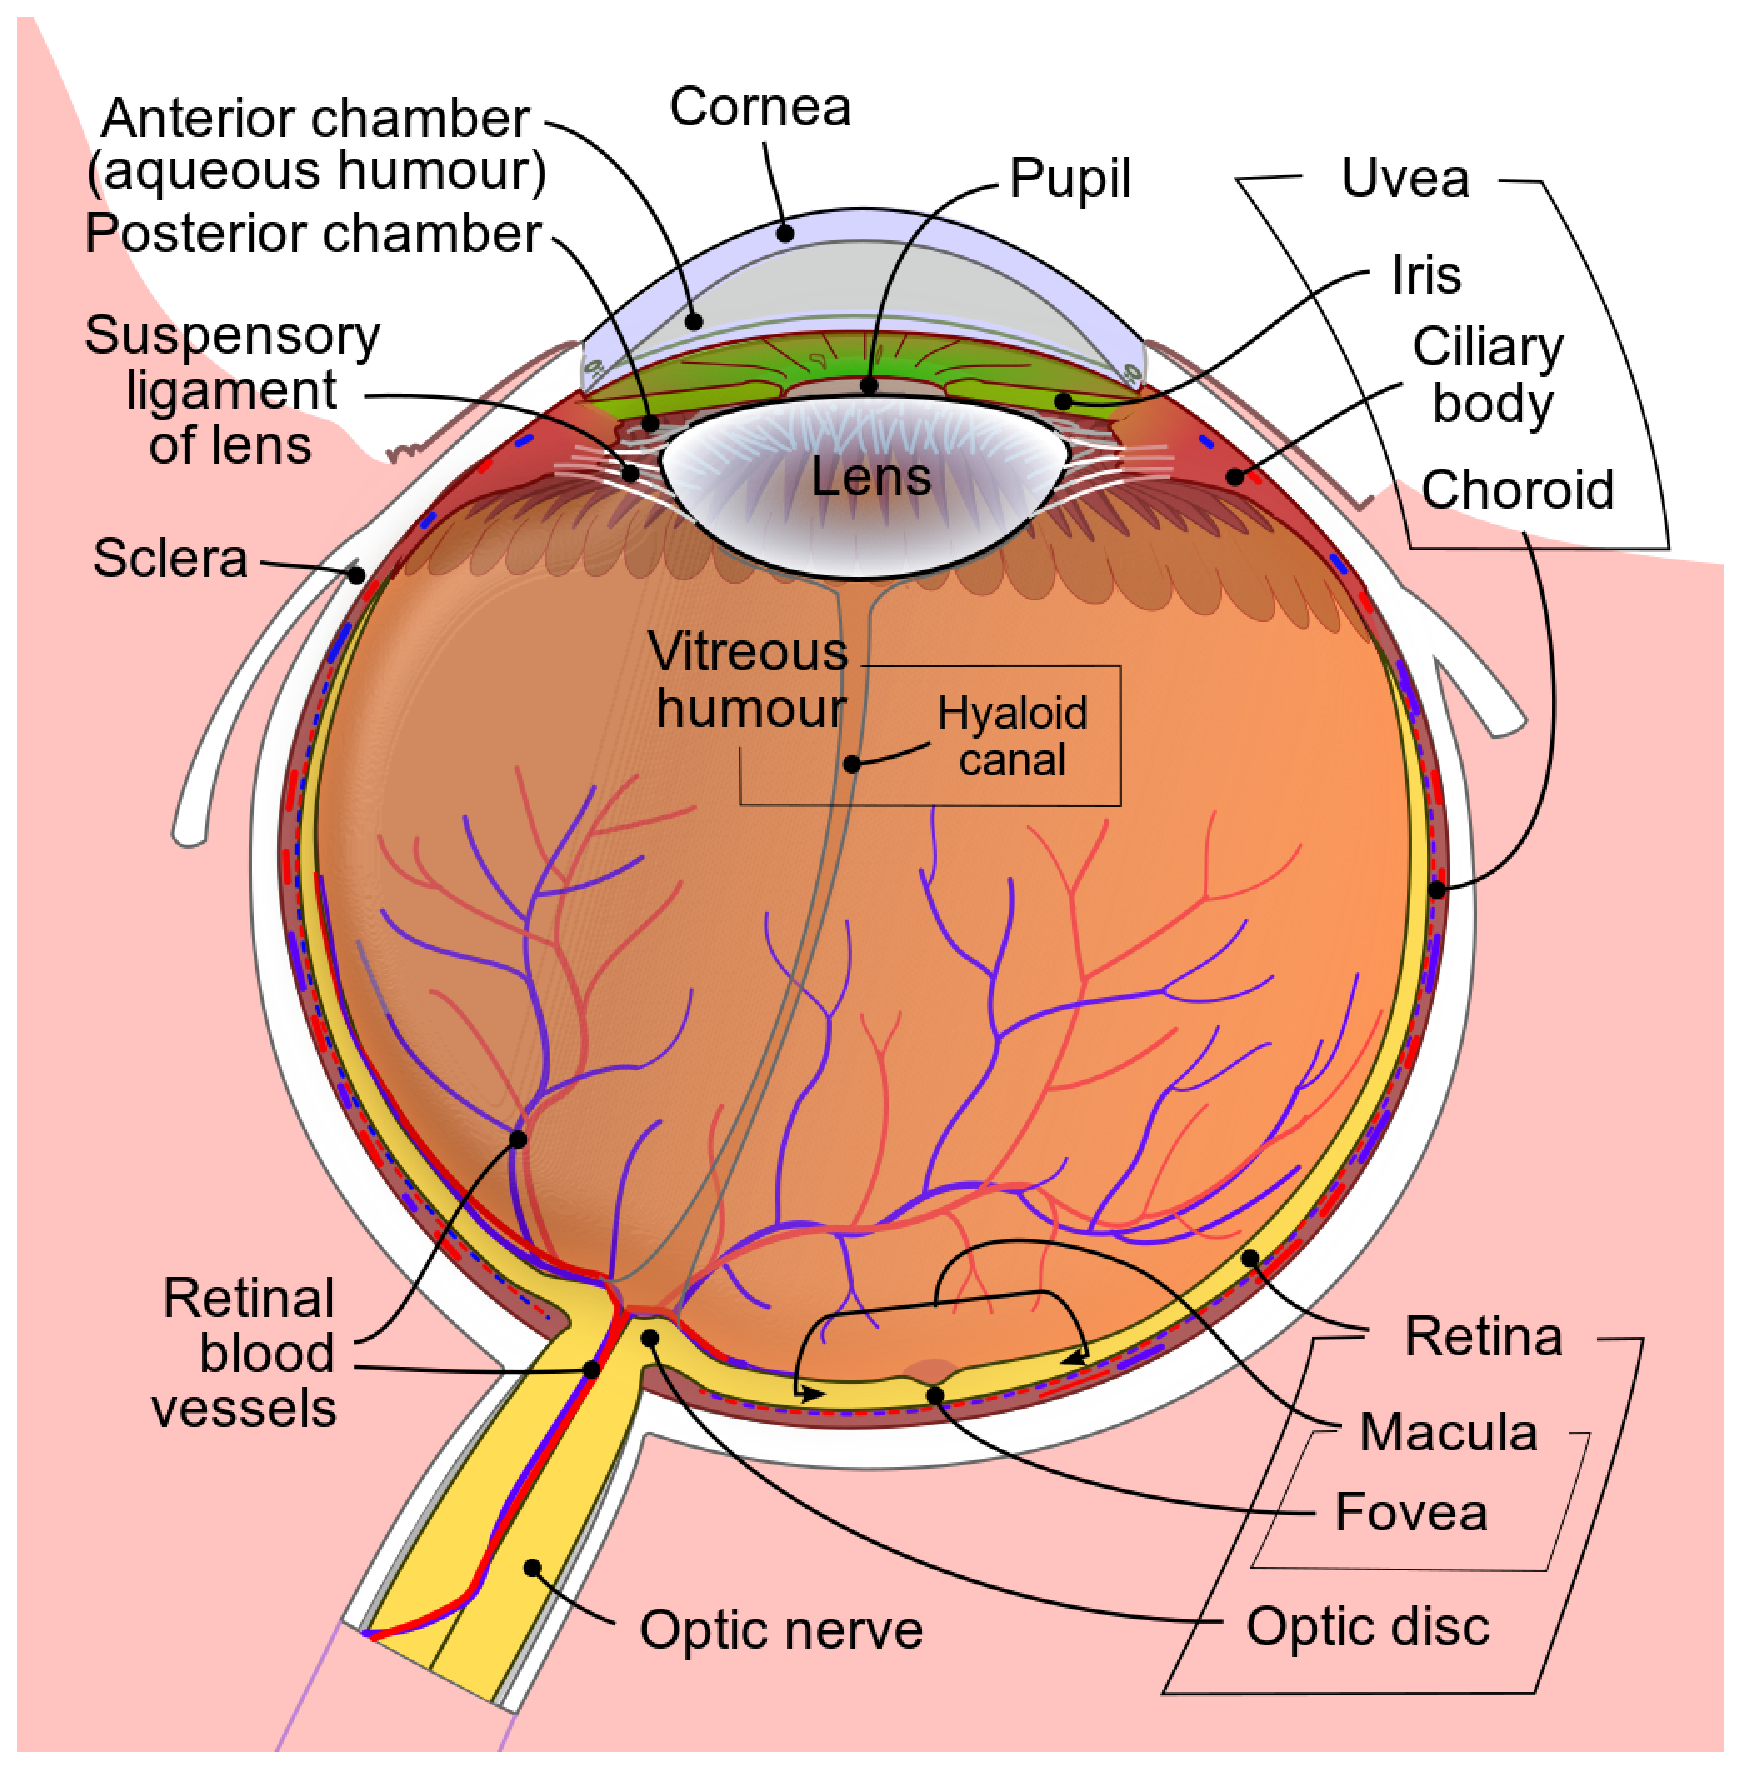
\includegraphics[width=0.8\textwidth]{Figures/chapter_introduction/eye_en.eps}
	\caption[Schematic diagram of the human eye]{Schematic diagram of the human eye (source commons.wikimedia.org)}
	\label{back:fig:eye}
\end{figure}

Diabetes is a disorder of the body due to its inability of producing or responding to the hormone insulin, resulting in abnormal metabolism of carbohydrates and elevated levels of glucose in the blood. Such high blood glucose levels can damage blood vessels and nerves, increasing the probability in diabetic patients of developing other derived diseases, like Diabetic Retinopathy. 

Diabetes can be of two different types: type 1 and 2. Type 1 is an autoimmune disease that causes the insulin producing beta cells in the pancreas to be destroyed, preventing the body from being able to produce enough insulin to adequately regulate blood glucose levels. Because type 1 diabetes causes the loss of insulin production, it therefore requires regular insulin administration. Type 2 is a metabolic disorder that results in hyperglycemia, ie. high blood glucose levels, due to the body either being ineffective at using the insulin it has produced or being unable to produce enough insulin. Type 2 diabetes is characterized by the body being unable to metabolize glucose, leading to high levels of blood glucose, which over time, may damage the organs of the body. \citep{www.diabetes.co.uk}

Diabetic Retinopathy is an associated disease derived from diabetes. It is caused by the damage of the small blood vessels of the retina. Due to diabetes disease related secondary effects, retinal blood vessels can break down, leak or become blocked; affecting the transport of nutrients and oxygen to parts of the retina, causing impaired vision over time. Due to the blockages, abnormal blood vessels can grow on the retina surface, causing an increment of the probability of bleeding and liquid leakages. Such structural changes can result initially in vision blurring and in last stages, even in retinal detachment and/or glaucoma. 

During the first two decades of the diabetes disease, nearly all patients with type 1 and more than 60\% of patients with type 2 diabetes, will develop a retinopathy \citep{fong2004retinopathy}. 

\subsection{Retina health evaluation}

There are several tests that a doctor may perform to evaluate retina eye health:

An \emph{ophtalmoscope} is a specialized type of microscope that allows the inspection of the vitreus, retina and other internal structures of the eye. With this instrument is possible to create a mirrored image of the various portions of the eye.

A \emph{visual field} or \emph{perimetry test}, mesures the ability of the examined eye to see straight ahead and the peripheral vision. The purpose of this test is to determine if there are any peripheral vision areas that are developing blind spots.

\emph{Fluorescein angiography} allows the doctor to inspect retina blood vessels. A vegetable-based dye is injected into patient blood stream. As blood circulates in the retina, a series of quick, sequential photographs of the eye are taken. These photographs provide useful information about its condition. Fluorescein angiography is one of the most important tests performed for determining the diagnosis and treatment of retinal disorders.

\emph{B-scan ultrasound} uses high frequency sound waves to view the back portions of the eye. This technology provides a full surface view of the eye that can be also used for retina condition evaluation.

\emph{Fundus photography} utilizes special cameras to document and track the progress of certain retinal diseases, like diabetic retinopathy, as well as monitor its treatment. This type of images are the used in this thesis for creating the automatic diagnostic system.

\subsubsection{Fundus photography}

Fundus photography is a technique for capturing the internal part of the back of the eye. This technique allows the visualization of main structures present in the back of eye interior, ie. center and peripherical retina, the optic disc and the macula.

Figure \ref{back:fig:fundus_camera} shows a photography of a typical camera used for capturing eye fundus images.

\begin{figure}[ht!]
	\centering
	\includegraphics[width=0.75\textwidth]{Figures/chapter_introduction/fundus_camera.jpg}
	\caption[Typical aspect of a fundus eye camera]{Typical aspect of a fundus eye camera (source commons.wikimedia.org)}  
	\label{back:fig:fundus_camera} 
\end{figure}

Figure \ref{back:fig:fundus_image_left_right_normal} shows an example of the fundus photography of both eyes of a healthy patient. In such images, it can be identified zones like central and peripherical retina, macula (darker part located at the center) and the optic disc (white spherical structure inside the retina).

\begin{figure}[ht!]
	\centering
	\scalebox{1.0}{
		\begin{subfigure}[b]{0.4\textwidth}
			\centering
			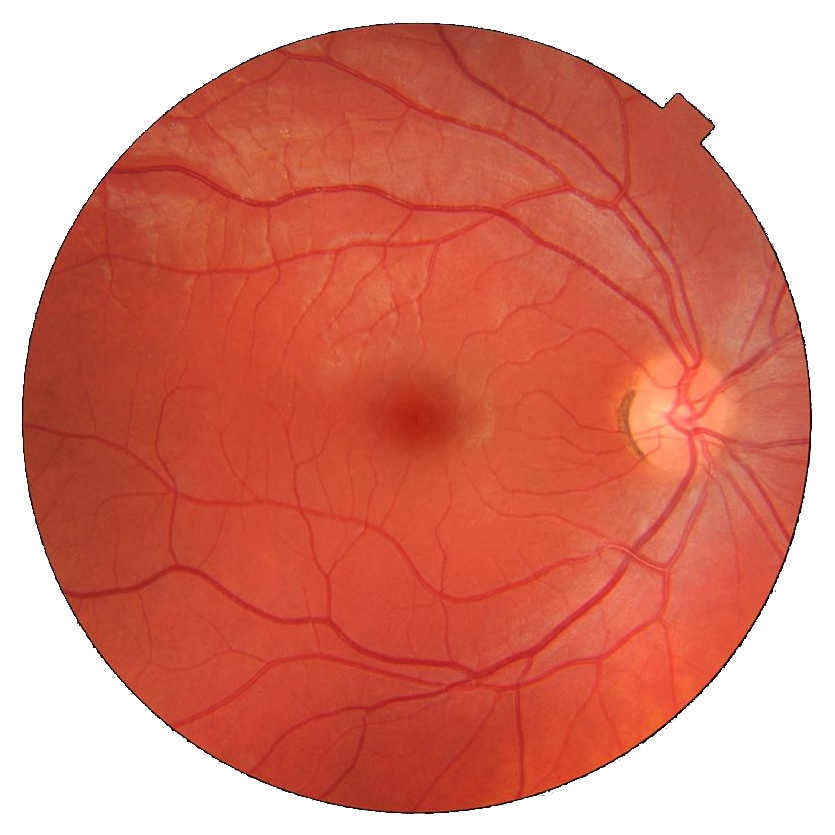
\includegraphics[width=\textwidth]{Figures/chapter_introduction/fundus_normal_eye_right.eps}
		\end{subfigure}
		\hfill    
		\begin{subfigure}[b]{.4\textwidth}
			\centering
			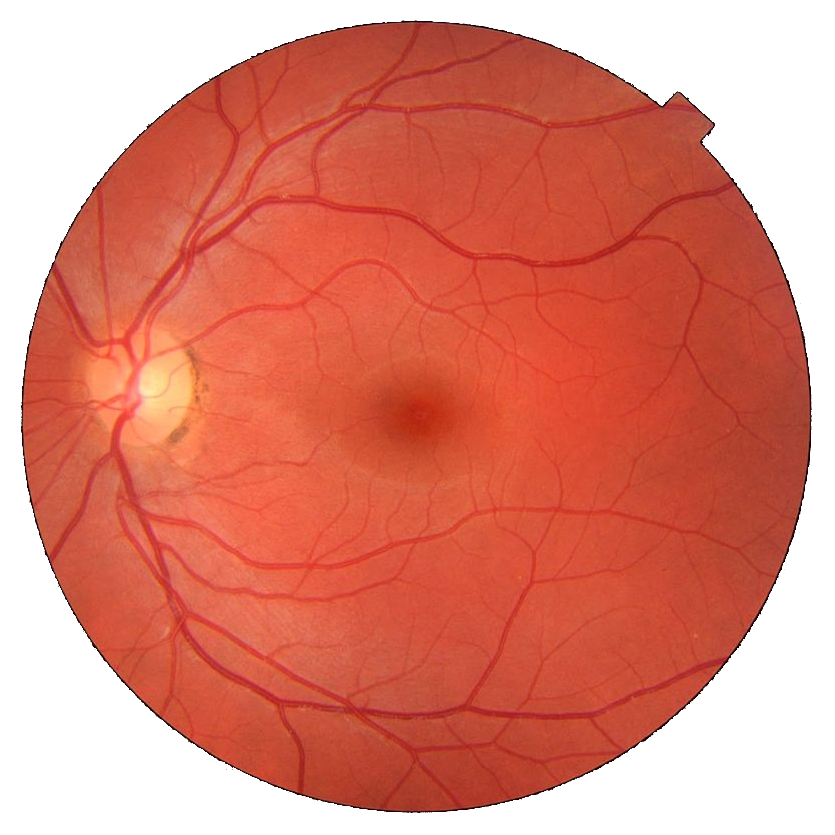
\includegraphics[width=\textwidth]{Figures/chapter_introduction/fundus_normal_eye_left.eps}\\
		\end{subfigure}
	}
	\hfill 
	\caption[Eye fundus images taken from a healthy patient]{Left and right eye fundus images taken from a healthy patient (source commons.wikimedia.org)}  
	\label{back:fig:fundus_image_left_right_normal} 
\end{figure}

With this type of photography is possible to identify, if they exist, the location and type of lesions and to infer from them a diagnostic.

%-----------------------------------
%	SUBSECTION 1
%-----------------------------------
\subsection{Diabetic retinopathy grading and classification}

Accurately grading diabetic retinopathy can be a significant challenge for a untrained person. Medical community establishes a standardized classification based on four severity stages \citep{diaclass} determined by the type and number of lesions (as micro-aneurysms, hemorrhages and exudates) present in the retina: class 0 referring to no apparent Retinopathy, class 1 as a Mild Non-Proliferative Diabetic Retinopathy (NPDR), class 2 as Moderate NPDR, class 3 as a Severe NPDR and class 4 as a Proliferative DR. 

Any of the stages can have no or few symptoms. Therefore, periodic dilated eye examinations are crucial for the detection and evolution study of the disease. Furthermore, diabetic macular edema can develop at any of these stages due to damaged and leaky blood vessels, affecting patient vision quality.

In the following sections diabetic retinopathy disease levels \citep{diaclass} are described:


\subsubsection*{No apparent diabetic retinopathy (class 0)}

The exams done to the fundus images of this class does not show any abnormality, either in the form of micro-aneurysms or in more complex forms. A diabetic patient with no retinopathy has a $<1\%$ chance of developing a PDR in the next four years \citep{klein2009wisconsin}.

\subsubsection*{Mild non-proliferative diabetic retinopathy (class 1)}

This is the earliest stage of the disease. In this stage, micro-aneurysms are the only abnormality found in exams. Class 1 diabetic patients have a $<5\%$ chance of developing a PDR in the next four years \citep{klein2009wisconsin}.

\begin{figure}[ht!]
	\centering
	\includegraphics[width=\textwidth]{Figures/chapter_background/classes/class1.png}
	\caption{Sample image of a Mild NPDR (class 1)} 
	\label{back:fig:class1_sample} 
\end{figure}

Figure \ref{back:fig:class1_sample} shows image EyePACS 11736\_left, tagged as 1 and classified as 1 by our best predictive model. We show lesion map generated by our models described in chapter \ref{Chapter:Interpretation}.

\subsubsection*{Moderate non-proliferative diabetic retinopathy (class 2)}

Moderate NPDR contains dot blot hemorrhages or microaneurysms in at least one quadrant with or without cotton-wool spots, venous beading, or intraretinal microvascular abnormalities (IrMA) but less than the 4:2:1 rule that defines the severe case nd that is explained below.

\begin{figure}[ht!]
	\centering
	\includegraphics[width=\textwidth]{Figures/chapter_background/classes/class2.png}
	\caption{Sample image of a Moderate NPDR (class 2)} 
	\label{back:fig:class2_sample} 
\end{figure}

Figure \ref{back:fig:class2_sample} shows image EyePACS 681\_right, tagged as 2 and classified as 2 by our best predictive model. We show lesion map generated by our models described in chapter \ref{Chapter:Interpretation}.

\subsubsection*{Severe non-proliferative diabetic retinopathy (class 3)}

Exam findings of the severe NPDR are characterized by any of the following cases:

\begin{itemize}
	\item 20 or more intraretinal hemorrhages (dot blot hemorrahages) in each of all four quadrants
	\item Definite venous beading in 2 or more quadrants
	\item Prominent intraretinal microvascular abnormality (IRMA) in one or more quadrants
\end{itemize}

These three points are called the 4:2:1 rule because the abnormalities are required to be present in at least 4, 2 and 1 retina quadrants respectively. Patients with severe NPDR have a $17 \%$ chance of developing high-risk PDR within one year, and $40\%$ chance of high-risk PDR within three years.

\begin{figure}[ht!]
	\centering
	\includegraphics[width=\textwidth]{Figures/chapter_background/classes/class3.png}
	\caption{Sample image of a Severe NPDR (class 3)} 
	\label{back:fig:class3_sample} 
\end{figure}

Figure \ref{back:fig:class3_sample} shows image EyePACS 1561\_left, tagged as 3 and classified as 3 by our best predictive model. We show lesion map generated by our models described in chapter \ref{Chapter:Interpretation}.


\subsubsection*{Proliferative diabetic retinopathy (class 4)}

This is the most advanced stage of the disease. In this stage, new, fragile \& abnormal blood vessels grow on the retina or optic nerve. These blood vessels can leak, affecting vision quality. Exams find either a definite neovascularization, or pre-retinal or vitreous hemorrhages. 
%-----------------------------------
%	SUBSECTION 2
%-----------------------------------

\begin{figure}[ht!]
	\centering
	\includegraphics[width=\textwidth]{Figures/chapter_background/classes/class4.png}
	\caption{Sample image of a PDR (class 4)} 
	\label{back:fig:class4_sample} 
\end{figure}

Figure \ref{back:fig:class4_sample} shows image EyePACS 11854\_left, tagged as 4 and classified as 4 by our best predictive model. We show lesion map generated by our models described in chapter \ref{Chapter:Interpretation}.


\section{Evaluation measures for disease grading}

An objective measure of the classification capabilities of a human or machine system requires the derivation of index measures that enable an exact measure of its performance. Even the most easiest classification task, ie. binary classification, requires the usage of many different indexes to find a good approximation of classification performance. For binary classification, instances of a set are classified as belonging or not to a class. Four possible outcomes can occur: a positive class being correctly classified (true positive, TP), a positive class being incorrectly classified (false positive, FP), a negative class being correctly classified (true negative, TN) and a negative class being incorrectly classified (false negative, FN). Furthermore, the prediction set can be balanced, ie. having the same number of elements of true positive and negative class or can be unbalanced having more instances of one class than another, producing a difference between absolute and relative results. All these variables make difficult to use a unique index for measuring the prediction capabilities. This is the reason why many different indexes exist, even for binary classification. Here below a brief description of the more used indexes for binary classification is presented.

\subsection{Confusion matrix}

The four possible outcomes, defined above, can be represented in a contingency table, known as \emph{confusion matrix}. Table \ref{back:tab:confusion_matrix_example} shows how information is represented in the table. 

\begin{table}[ht]
	\centering
\begin{tabular}{l|l|c|c|c}
	\multicolumn{2}{c}{}&\multicolumn{2}{c}{True class}&\\
	\cline{3-4}
	\multicolumn{2}{c|}{}&Positive&Negative&\multicolumn{1}{c}{Total}\\
	\cline{2-4}
	\multirow{2}{*}{Predicted class}& Positive & $TP$ & $FN$ & $TP+FN$\\
	\cline{2-4}
	& Negative & $FP$ & $TN$ & $FP+TN$\\
	\cline{2-4}
	\multicolumn{1}{c}{} & \multicolumn{1}{c}{Total} & \multicolumn{1}{c}{$TP+FP$} & \multicolumn{    1}{c}{$TN+FN$} & \multicolumn{1}{c}{$Total$}\\
\end{tabular}
	\caption{Binary confusion matrix}
\label{back:tab:confusion_matrix_example} 
\end{table}

Confusion matrix summarizes all information about the problem. All other indexes are derived from the information showed in this table. Confusion matrix can be easily generalized for its usage in multi-class classification cases, just adding as many rows and columns as classes to predict.

\subsection{Sensitivity and Specificity}

Sensitivity and Specificity are the most important indexes derived from confusion matrix.  Sensitivity (eq. \ref{back:eq:sensitivity}), also known as recall, hit rate or true positive rate, measures the proportion of actual positives that are correctly identified as such. Specificity (eq. \ref{back:eq:specificity}), also known as selectivity or true negative rate, measures the proportion of actual negatives that are correctly identified as such. Mathematically is expressed as: .

\begin{equation}
Sensitivity = \frac{TP}{P}
\label{back:eq:sensitivity}
\end{equation}

\begin{equation}
Specificity = \frac{TN}{N}
\label{back:eq:specificity}
\end{equation}

In medical diagnosis, sensitivity measures the model ability to correctly identify those with the disease, whereas specificity measures the model ability to correctly identify those without the disease. 

\subsection{Positive and Negative Predictive Value}

Positive Predictive Value (PPV) (eq. \ref{back:eq:ppv}), also known as precision, measures of the proportion of correctly classified positive cases over the total number of predicted positives. It allows the identification of too conservative models. Negative Predictive Value (NPV) (eq. \ref{back:eq:npv}) measures the same in negative cases.

\begin{equation}
PPV=\frac{TP}{TP+FP}
\label{back:eq:ppv}
\end{equation}

\begin{equation}
NPV=\frac{TN}{TN+FN}
\label{back:eq:npv}
\end{equation}


\subsection{False Positive and Negative Rates}

False Positive Rate (eq. \ref{back:eq:fpr}) and False Negative Rate (eq. \ref{back:eq:fnr}) indexes measure the rate of false values reported by the model. In statistical hypothesis testing these indexes are known as type I and II errors respectively. They are of common use in medical diagnosis, being a very important indexes for defining strategies of screening or testing.

\begin{equation}
FPR=\frac{FP}{N}
\label{back:eq:fpr}
\end{equation}

\begin{equation}
FNR=\frac{FN}{P}
\label{back:eq:fnr}
\end{equation}

\subsection{False Discovery and Omission Rates}

False Discovery Rate (eq. \ref{back:eq:fdr}) measures the proportion false positives which are incorrectly accepted. False omission rate (eq. \ref{back:eq:for}) measures the proportion of false negatives which are incorrectly rejected. Both measures complement FPR and FNR.

\begin{equation}
FDR=\frac{FP}{FP+TP}
\label{back:eq:fdr}
\end{equation}

\begin{equation}
FOR=\frac{FN}{FN+TN}
\label{back:eq:for}
\end{equation}

\subsection{Accuracy}

Accuracy (eq. \ref{back:eq:acc}) measures the proportion of true predictions (positive or negative) over the total of population. This measure can be misleading in unbalanced data sets giving too optimistic results due to the weight of predominant class.

\begin{equation}
ACC=\frac{TP+TN}{Total}
\label{back:eq:acc}
\end{equation}

\subsection{Balanced measures}

Each one of the indexes defined above give a partial information about the classification, this is the reason why a combination of some of them, and not its individual values alone, must be taken into account to make a correct evaluation of model performance. In the quest of finding a unique index that summarizes global performance, a set of meta-indexes have been proposed. These meta-indexes combine the information given by a set of indexes to, in this way, give a unique index with an overall performance evaluation. In between these indexes are: $F_\beta$, Matthews correlation coefficient (MCC) \citep{sammut2011encyclopedia}.

\paragraph{$F_\beta$} (eq. \ref{back:eq:f_measure}) is an harmonic mean between specificity and sensitivity. $\beta$ is a constant that allows to weight the relative importance of both components. For giving the same importance to both variables, $\beta$ is set to 1. 

\begin{equation}
F_\beta = (1 + \beta^2) \frac{sensitivity \cdot specificity}{\beta^2 \cdot specificity + sensitivity}
\label{back:eq:f_measure}
\end{equation}

\paragraph{MCC} (eq. \ref{back:eq:mcc}) acts as a correlation coefficient between observed and predicted values. MCC is related to the chi-square statistic for a 2x2 contingency table. 

\begin{equation}
MCC = \frac{TP \cdot TN + FP \cdot FN}{\sqrt{(TP \cdot FP)(TP \cdot FN) (TN \cdot FP)(TN \cdot FN)}}
\label{back:eq:mcc}
\end{equation}


\subsection{The Kappa family of statistics}

Ordinal Regression is a particular case of multi-class classification where an ordering of the classes can be established a priori, based on some underlying properties present in data.

In medical diagnosis, it is a typical situation the use of an ordinal or nominal classification scale for defining the severity of patient diseases. Frequently, such scales are designed for identifying the gradation of disease level from mild cases to the most severe, being then a particular case of an ordinal regression.

A typical situation in the definition of such gradation classes is the inherent existence of some subjectivity. Normally, the underlying properties that define the classification are not completely observable or cannot be completely identified, causing even experts to differ to some extent in its conclusions, requiring the usage of an index that allows the objective measure of the level of agreement between experts.

Kappa family of statistics \citep{sim2005kappa} are a way of measuring such inter-rater and intra-rater agreement, ie. diagnostics reliability. Main purpose of the kappa derived statistics is to measure of "true" agreement. When a set of experts evaluate a fact, there are mainly to sources of possible agreement: one coming from expertise and another from chance. Kappa index discounts the probability of agreement by chance, being then a pure measure of "true" agreement.

In its binary classification form and for evaluation of two experts, kappa can be expressed as eq. \ref{back:eq:kappa_bin}.

\begin{equation}
\kappa = \frac{P_o - P_c}{1 - P_c}
\label{back:eq:kappa_bin}
\end{equation}

being $P_o$ the proportion of observed agreement and $P_c$ the proportion of agreement by chance. The range of possible values of kappa is of -1 to +1. Denoting $\kappa=-1$ complete disagreement, $\kappa=0$ random agreement and $\kappa=+1$ complete agreement between raters.

\paragraph{Kappa for multi-class classification.} Kappa coefficient can be extended for its use with more than 2 ordinal categories. When more than two classes are present, disagreement can be expressed by the distance between predictions of both raters. Weighted kappa is the multi-class version of original kappa, where the discrepancy is penalized by a weight that is a function of the distance between both predictions. The most common weight strategy used is the quadratic, where weights used are proportional to the square of the distance between predictions of both raters. In such case, the index is known as \emph{Quadratic Weighted Kappa}, QWK or $\kappa$ indistinctly \citep{cohen1968weighted}. This index is the most commonly used by medical community and it is the main one used in this thesis for performance evaluation.

\begin{equation}
\kappa = \frac{\sum \omega f_o - \omega f_c}{n - \sum \omega f_c}
%\kappa = 1 - \frac{\sum_{i,j} \omega_{i,j} P_{i,j}}{\sum_{i,j} \omega_{i,j} E_{i,j}}
\label{back:eq:kappa_qwk}
\end{equation}

Equation \ref{back:eq:kappa_qwk} shows the expression of quadratic weighted kappa, where $\sum \omega f_o$ is the sum of weighted observed frequencies in the confusion matrix cells, and $\sum \omega f_c$ the sum of weighted frequencies expected by chance in the confusion matrix cells. In case of using linear weights, $\omega = 1 - \frac{|i-j|}{k-1}$ and in case of quadratic weights, $\omega = 1 - \big( \frac{i-j}{k-1} \big)^2$.  %Being $\omega_{i,j}$ the weight applied to the proportion of predictions rated by first rater as $i$ and for second rater as $j$ that, by definition is equal to $\omega_{i,j} = (i - j)^2$. 

Alternatively, QWK can be defined in terms of observation and expectation histogram matrices. For $N$ classes, a NxN observation matrix $O$ is constructed, such that $O_{i,j}$ correspond to the number of elements rated as class $i$ by rater 1 and as class $j$ by rater 2. A NxN expectation matrix $E$ is also calculated as the outer product between each rater's histogram vector, normalized such that $E$ and $O$ have the same sum. Representing the weights as $\omega = \frac{(i-j)^2}{(N-1)^2}$, kappa can be calculated as:

\begin{equation}
\kappa = 1 - \frac{\sum_{i,j} \omega_{i,j} O_{i,j}}{\sum_{i,j} \omega_{i,j} E_{i,j}}
\label{back:eq:kappa_qwk2}
\end{equation}

\paragraph{Kappa interpretation.} In \citep{landis1977measurement} the next standards of agreement are proposed: $\kappa \leq 0$ indicating poor agreement, $0.01 \leq \kappa \leq 0.20$ slight, $0.21 \leq \kappa \leq 0.40$ fair, $0.41 \leq \kappa \leq 0.60$ moderate, $0.61 \leq \kappa \leq 0.80$ substantial and $\kappa \geq 0.81$ almost perfect. Value of $kappa$ is influenced by the weighting applied and by the number of classes, bias and prevalence, this is the reason why kappa values are not comparable across variables having different prevalence or bias \citep{sim2005kappa}. In the case of diabetic retinopathy disease grading, using QWK, the inter-rating agreement between expert ophthalmologists is about $0.80$. For the purpose of this thesis, such value ($\kappa = 0.80$) is the standard of reference our models are compared against.

\subsection{How to define human performance}

A key factor for evaluation of machine performance against humans is the standard used to measure the last one. In the context of medical classification, the next comparison standards can be used:

\begin{enumerate}
\item A person (not a doctor)
\item A general doctor
\item A specialized doctor
\item A highly experienced specialized doctor
\item A team of highly experienced specialized doctors
\end{enumerate}

The team of highly experienced specialized doctors can be approximated to the \emph{Bayes Optimal Error} \citep{fukunaga2013introduction}, \citep{tumer1996estimating}. In any case, it is important to define the standard we are comparing against. For the purpose of this thesis, human performance is established as the given by a \emph{highly experienced specialized doctor}.

\section{Machine Learning}

Machine Learning is a Computer Science discipline, sub-field of Artificial Intelligence, that include all the tools and techniques used for enabling computers to learn from data and, from a more ambitious perspective, giving computers the ability of acting without being explicitly programmed.  

All tools and techniques available in the discipline can be classified according on the type of learning algorithm that they implement: supervised, unsupervised and reinforced learning.

\paragraph{Supervised learning} algorithms require all the instances of the training set to be labeled. From this previous knowledge the algorithm is able to learn and generalize, being able to predict new never seen before samples. From a probability perspective these type of algorithms learn a conditional distribution, ie. $P(c|X)$, being $c$ the class to predict and $X$ the sample.

\paragraph{Unsupervised learning} algorithms allow the learning of underlying regularities present in the training set without requiring labeling of the individual instances. From a probability perspective, such models are able to learn the joint distribution of the population represented by the training set, ie. $P(X)$, being $X$ the sample.

\paragraph{Reinforcement learning} algorithms give models the capacity of learning from environment, ie. accumulating experience from its interaction with the surroundings. Such models are goal oriented,  having an internal representation of the environment that is updated periodically with the objective of maximizing gain.

\subsection{Supervised Learning}

In this thesis we used supervised learning techniques for learning from data. As previously stated, in this learning paradigm a \emph{labeled training set} is used as a foundation for learning general representations that can be used for generalizing behaviors and inferring then new labels in never seen before data.

\subsubsection{Classification vs Regression}

The objective of supervised learning is the learning of a conditional probability distribution in the form of $P(c|X)$. Depending on the nature of the variable to be predicted, it can be differentiated between classification or regression. Fundamentally, classification is about a disjoint class label prediction and regression is about a quantity prediction. Ordinal regression is a particular case of classification, where some a priori class ordinality can be established.

\subsubsection{Dataset management}

In supervised learning, the source of knowledge is represented by a labeled data set. The probability distribution of the population that it is supposed to be predicted is assumed to be represented by a sample, ie. a labeled data set. The design process of a predictive model has two parts: building the model (ie. training) and statistical evaluation of its performance. Performance evaluation require the usage of a never seen before data set, so the original full data set is required to be split in two parts: one for training (called \emph{training set}) and another for testing (called \emph{test set}). Both train and test set must be big enough either for training good models or for having a high statistical confidence of its generalization capabilities.

\subsubsection{Strategies for hyper-parameter optimization}

Frequently, supervised learning models have parameters that must be fixed before learning. In such cases, model performance can change dramatically depending on the selected parameters, requiring also a meta-learning parameter optimization for selection of the highest performance model, more commonly known as hyper-parameter optimization. 

Different strategies can be followed in order to optimize such meta-parameters:

\paragraph{Hold Out method:} This method splits original training data set using random sampling without repetition into 2 subsets. The first called training set is used for fitting the model/s, the second one, called validation set is used for hyper-parameter optimization and for model selection, not only between hyper-parameters but also between different types of models. As a rule of thumb, training set use to have between 50\% to 70\% of the data and validation set between 50\% to 30\%.

\paragraph{K-fold cross validation:} The original training set is split in $K$ folds of the same size using random sampling without repetition. The model/s are trained $K$ times, each one of them using as training set $K-1$ folds and $1$ (the not used one) as a validation set. Prediction error is the average of $K$ individual errors. Error variance can be used as a measure of the model stability. The advantage of this method is that it matters less how the data is divided, ie. the model is less prone of having selection bias. After choosing the best model hyper-parameters and/or model, a retrain with the whole data set is recommended.

\paragraph{Leave one out cross-validation:} It is a type of K-fold cross validation where it is hold out only one sample each time. It is a good way to validate, but requires a high computation time.

\paragraph{Bootstrap methods:} It randomly draws data sets from the original sample. Each sample size is equal to the original training size. Each model/s with its particular hyper-parameters is fitted using the bootstrapped samples. Model/s are examined with the out-of-bag data, ie. data not selected in each bootstrap.

\subsection{Algorithms used in supervised machine learning}

The most widely used learning algorithms can be divided into the next categories:

\begin{itemize}
\item Linear / Logistic regression
\item Support Vector Machines
\item Probabilistic Graphical Models
\item Decision trees related algorithms
\item Deep Learning (Multilayer Perceptron, Neural Networks)
\item Others (clustering, association rules, inductive logic, representation learning, similarity and metric learning, sparse dictionary learning, genetic algorithms, etc.)
\end{itemize}

\paragraph{Linear/Logistic Regression} are regression and classification algorithms, where a linear combination of the inputs is optimized for least squares error minimization in the first case and for cross entropy minimization in the second.

\paragraph{Support Vector Machines} are similar to linear/logistic regression but using a different optimization function. They minimize the Hinge loss, giving as a result maximum-margin classifiers. Support vector machines can be used as linear classifiers but also as a non-linear ones, substituting its features with so-called kernels, that are non-linear functions of the features and training set samples. 

\paragraph{Probabilistic Graphical Models} are a set of models based on probabilistic conditional dependency graphs that use bayesian rules for model construction and inference.

\paragraph{Decision Trees based models} are a set of very effective algorithms based on the usage of weak learners like decision trees for constructing very powerful predictors combining them using bagging or boosting techniques. This category include algorithms like Random Forest or Gradient Boosting.

\paragraph{Deep Learning} also known as Artificial Neural Networks or Multilayer Perceptrons, is a set of Machine Learning techniques for automatically constructing models from the underlying distribution represented by a large set of examples, using multiple levels of representation (in the form of layers), with the final objective of mapping a high-multidimensional input into a smaller multidimensional output (f: $\mathbb{R}^{n} \mapsto \mathbb{R}^{m}, n \gg m$). This mapping allows the classification of multidimensional objects into a small number of categories. The model is composed by many neurons that are organized in layers and blocks of layers, using a cascade of layers in a hierarchical way. Every neuron receives the input from a predefined set of neurons. Every connection has a parameter that corresponds to the weight of the connection. The function of every neuron is to make a transformation of the received inputs into a calculated output value. For every incoming connection, the weight is multiplied by the input value received by the neuron and the aggregated value that used by an activation function that calculates the output of the neuron. Parameters are usually optimized using a stochastic gradient descent algorithm that minimizes a predefined loss function. Network parameters are updated after back-propagating the loss function gradients through the network. These hierarchical models are able to learn multiple levels of representation that correspond to different levels of abstraction, which enables the representation of complex concepts in a compressed way \citep{nature-deep-learning}, \citep{888}, \citep{Bengio:2013:RLR:2498740.2498889}, \citep{bengio-2009}. The models used in this thesis are based mainly in Deep Learning.

\subsection{Pattern recognition}

\subsubsection{Traditional models of pattern recognition}

The traditional model for pattern recognition since the 50's were based on a fix design of a set of important features manually engineered or derived from a fixed kernel (Fig. \ref{back:fig:trad_pat_rec}). Such kernels allowed the extraction of texture, statistic, position, geometry features that were posteriously combined with a simple classifier. A great diversity of methods for feature extraction exist as the local binary pattern, histogram of oriented gradients, gray level co-occurence matrix, gabor filters, between others. In the classification phase it was common practice to use k-nearest neighbors, linear discriminant analysis, support vector machines or decision trees derived algorithms like random forest or gradient boosting.

\begin{figure}[!h]
	\centering
	\smartdiagramset{back arrow disabled=true}
	\resizebox{.9\linewidth}{!}{\smartdiagram[flow diagram:horizontal]{Image Input, Hand-Crafted Feature Extractor, 'Simple'\\Classifier, Class}}
	\caption{Traditional pattern recognition scheme}
	\label{back:fig:trad_pat_rec}
\end{figure}

Such pattern recognition pipeline required a lot of labor time for designing the appropriate filters for every particular application.

\subsubsection{Deep Learning for pattern recognition}

Deep learning for pattern recognition represents a change of the design paradigm. Instead of hand-crafting features, a fully trainable model is designed, that is the combination of a trainable feature extractor and a trainable classifier (Fig \ref{back:fig:dl_pat_rec}), creating a end-to-end automatic learner.

\begin{figure}[!h]
	\centering
	\smartdiagramset{back arrow disabled=true}
	\resizebox{.9\linewidth}{!}{\smartdiagram[flow diagram:horizontal]{Image Input, Trainable Feature Extractor, Trainable Classifier, Class}}
	\caption[Deep Learning pattern recognition scheme]{Deep Learning pattern recognition scheme (end-to-end learning)}
	\label{back:fig:dl_pat_rec}
\end{figure}

\subsubsection{Types of Deep Learning architectures}

Neural networks are the architectures lying under the term of deep learning. They are directed graphical models with a defined architecture formed by their building block, the neuron. We can differentiate between three typical base architectures: fully connected, convolutional and recurrent neural networks. Every designed network can be classified into one of such architectures or as combinations of them. Each one is suitable for different types of problems. Recurrent neural networks are optimized to be used for serially organized information, for example text or sound related problems. Convolutional neural networks are designed for local correlation exploitation, for example in the case of images. Fully connected layers are designed to be used in cases where all the information is equally important, for example in classification layers. The models designed in this thesis use mainly convolutional neural networks.

\subsubsection{Convolutional neural networks}

Convolutional neural networks (fig. \ref{back:fig:cnn}), firstly proposed successfully in \citep{lecun1989backpropagation} for handwritten image recognition, are the main type of network used in this thesis for diabetic retinopathy image classification and interpretation.

\begin{figure}[!htb]
	\centering
	\includegraphics[width=0.9\textwidth]{Figures/chapter_background/typical_cnn.png}
	\caption[High level representation of a typical convolutional neural network]{High level representation of a typical convolutional neural network (source: commons.wikimedia.org)}
	\label{back:fig:cnn}
\end{figure}

CNNs are a type of neural network specialized in exploiting the natural local correlations present in images. They are able to create local abstractions that are combined layer-by-layer forming more elaborated meta-abstractions, hopefully, being able to disentangle the information contained in the image, forming features that are useful for solving a particular classification/regression problem. 

As conventional neural networks, they are formed by a set of layers that are piled together. Each layer has a convolutional operator that allows the transformation of a input tensor into another one. The output tensor can pass through other transformations inside the same layer, like a batch-normalization, an activation function or reducing size functions like max-pooling or average pooling blocks. All these functions are parametric, ie. they have learnable parameters, that are tuned through a loss function optimization process with the objective of enhancing the classification/regression capabilities of the network. The characteristic building block of such type of network is the convolution operator.

\paragraph{Convolution operator} (fig. \ref{back:fig:convolution_operator}) is repeatedly applied to different localizations of the input. Parameters that define such operator are: a tensor of \emph{number of feature inputs x convolution width x convolution height x number of outputs}, \emph{horizontal and vertical padding} and \emph{horizontal and vertical stride}. Padding defines the number of pixels that must be added to the width and height of the input before applying it, ie. if the input has a \emph{width x height} original size, is extended for applying the operator to \emph{(width + 2 x padding width) x (height + 2 x padding height)}. The operator is applied in every location of the input with a separation between initial points of \emph{horizontal stride} and \emph{vertical stride}. The output value correspond to the linear combination of the convolution parameters with input values.

\begin{figure}[!ht]
	\centering
	\begin{subfigure}{0.2\textwidth}
		\includegraphics[scale=0.5]{Figures/chapter_background/convolution_operator/padding_strides_odd_00.pdf}
	\end{subfigure}
	~ % spacing  ~, \quad, \qquad
	\begin{subfigure}{0.2\textwidth}
	\includegraphics[scale=0.5]{Figures/chapter_background/convolution_operator/padding_strides_odd_01.pdf}
	\end{subfigure}
	~ % spacing  ~, \quad, \qquad
	\begin{subfigure}{0.2\textwidth}
	\includegraphics[scale=0.5]{Figures/chapter_background/convolution_operator/padding_strides_odd_02.pdf}
	\end{subfigure}
	~ % spacing  ~, \quad, \qquad
	\begin{subfigure}{0.2\textwidth}
	\includegraphics[scale=0.5]{Figures/chapter_background/convolution_operator/padding_strides_odd_03.pdf}
	\end{subfigure}
	\caption[Convolution operator of 3x3, stride 2, padding 1]{Convolution operator of 3x3 with stride 2 and padding 1 in both directions applied to a 6x6 input. Only one input and output features are shown \citep{dumoulin2016guide}.}
	\label{back:fig:convolution_operator}
\end{figure}

\paragraph{Pooling operators} (fig. \ref{back:fig:pooling_operator}) are other typical elements used in CNNs. They are used for reducing the size of feature maps. Max-pooling operators select from a predefined window the maximum value and discards the others. Average-pooling, selects the average. Both, are the most common strategies for reducing the size of feature maps.

\begin{figure}[!ht]
	\centering
	\begin{subfigure}{0.2\textwidth}
		\includegraphics[scale=0.5]{Figures/chapter_background/max_pooling/numerical_max_pooling_05.pdf}
	\end{subfigure}
	~ % spacing  ~, \quad, \qquad
	\begin{subfigure}{0.2\textwidth}
		\includegraphics[scale=0.5]{Figures/chapter_background/max_pooling/numerical_max_pooling_06.pdf}
	\end{subfigure}
	~ % spacing  ~, \quad, \qquad
	\begin{subfigure}{0.2\textwidth}
		\includegraphics[scale=0.5]{Figures/chapter_background/max_pooling/numerical_max_pooling_07.pdf}
	\end{subfigure}
	~ % spacing  ~, \quad, \qquad
	\begin{subfigure}{0.2\textwidth}
		\includegraphics[scale=0.5]{Figures/chapter_background/max_pooling/numerical_max_pooling_08.pdf}
	\end{subfigure}
	\caption[Max-pooling operator of 3x3, stride 1, padding 0]{Max-pooling operator of 3x3 with stride 1 and padding 0 in both directions applied to a 5x5 input. Only one input and output features are shown \citep{dumoulin2016guide}.}
	\label{back:fig:pooling_operator}
\end{figure}

\paragraph{Batch normalization} are another typical element used in CNN layers. It applies a normalization to the inputs that help to reduce covariate shift, increasing stability and acting as a regularizer \citep{batch-norm}.

\paragraph{Activation function} (fig. \ref{back:fig:activations}) is a key element of neural networks. ReLU is the most versatile, stable and used one. Sigmoid function, the most used one in the 80's, only used nowadays for certain types of output layers, due to its gradient descent vanishing problems. Without them, deep learning models would behave just like linear functions. In the 80s the most used activation function was the sigmoid, a smooth non-linear function, that is continously differentiable. Despite its interesting properties, it has a very important concern, called gradient vanishing problem \citep{glorot2010understanding}. Sigmoid first derivative becomes flat not far from the origin, affecting network loss optimization due to near-to-zero gradients. In \citep{nair2010rectified} ReLUs were used for improving Restricted Boltzmann Machines (RBMs), approximating stepped sigmoid units with ReLUs. In \citep{glorot2011deep} the authors compared the performance of Sigmoid, Tanh and ReLU arriving to the conclusion that despite Sigmoid being more plausible biologically, Tanh and ReLU were more suitable to be used as activation function for training multi-layer perceptrons. ReLU networks have better performance in general, despite its non-differentiability at zero and its hard non-linearity. Furthermore, ReLU networks lead to sparse representations, being beneficial, both because information is represented in a more robust manner and because it leads to significant computational efficiency. Moreover, the simplicity of the function and its derivative reduces calculation time, being of significant importance when working with big networks. The constant value of the gradient, helps avoiding the gradient vanishing problem, allowing the design of deeper networks. For then on, ReLU has become the default activation function for deep learning. Many other activation functions have been published, like LeakyReLU, but not introducing significant performance gains.

\begin{figure}[h!]
	\centering
	\begin{subfigure}{0.2\textwidth}
		\includegraphics[scale=0.6]{Figures/chapter_background/activation_functions/relu.pdf}
		\caption{ReLU}
	\end{subfigure} ~
	\begin{subfigure}{0.2\textwidth}
		\includegraphics[scale=0.6]{Figures/chapter_background/activation_functions/leakyrelu.pdf}
		\caption{leakyrelu}
	\end{subfigure} ~
	\begin{subfigure}{0.2\textwidth}
		\includegraphics[scale=0.6]{Figures/chapter_background/activation_functions/tanh.pdf}
		\caption{Tanh}
	\end{subfigure} ~
	\begin{subfigure}{0.2\textwidth}
		\includegraphics[scale=0.6]{Figures/chapter_background/activation_functions/sigmoid.pdf}
		\caption{Sigmoid}
	\end{subfigure}
	\caption{Typical activation functions used in Deep Learning}
	\label{back:fig:activations}
\end{figure}

\paragraph{Typical CNN architectures.} CNNs have been demonstrated to be very effective in solving complex classification, detection and segmentation problems. Table \ref{back:fig:imagenet_models} shows a summary of the most successful Imagenet \citep{imagenet_cvpr09} prediction standardized architectures sorted by its performance solving the complex Imagenet classification task. The more successful network presented in the table is \emph{InceptionResNetV2} having more than 55 million of parameters. \emph{Xception} has a similar accuracy using less than a half of parameters. \emph{MobileNetV2}, an architecture designed to be used in mobile devices, with only 3.4 million of parameters has an accuracy similar to the achieved with older architectures as \emph{VGG16} and \emph{VGG19}, that used more than 100 million of parameters.

\begin{table}[h!]
	\centering
	\scalebox{0.55} {
	\begin{tabular}{lccccccc}
		\textbf{Model}    & \textbf{Input size} & \textbf{\shortstack{Imagenet\\Top-1\\Accuracy}} & \textbf{Params} & \textbf{Depth} & \textbf{Residual} & \textbf{Publication} & \textbf{Source} \\
		\hline
		InceptionResNetV2 & (299,299,3)         & 0.804                            & 55.9M               & 572            & Yes               & 2016-02              & \citep{szegedy2017inception}          \\
		InceptionV4       & (299,299,3)         & 0.802                            & 55.9M               &                & No                & 2016-02              & \citep{szegedy2017inception}          \\
		Xception          & (299,299,3)         & 0.790                            & 22.9M               & 126            & Yes               & 2016-10              & \citep{chollet2017xception}          \\
		InceptionV3       & (299,299,3)         & 0.788                            & 23.8M               & 159            & No                & 2015-12              & \citep{szegedy2016rethinking}          \\
		DenseNet201       & (224,224,3)         & 0.770                            & 20.2M               & 201            & Dense             & 2016-08              & \citep{huang2017densely}        \\
		ResNet50          & (224,224,3)         & 0.759                            & 25.6M               & 168            & Yes               & 2015-12              & \citep{he2016deep}       \\
		DenseNet169       & (224,224,3)         & 0.759                            & 14.3M               & 169            & Dense             & 2016-08              & \citep{huang2017densely}        \\
		MobileNetV2 (1.4) & (224,224,3)         & 0.747                            & 6.9M                &                & Yes               & 2018-01              & \citep{sandler2018mobilenetv2}          \\
		DenseNet121       & (224,224,3)         & 0.745                            & 8M                  & 121            & Dense             & 2016-08              & \citep{huang2017densely}        \\
		VGG19             & (224,224,3)         & 0.727                            & 143.7M              & 26             & No                & 2014-09              & \citep{vggnet}          \\
		MobileNetV2       & (224,224,3)         & 0,720                            & 3.4M                &                & Yes               & 2018-01              & \citep{sandler2018mobilenetv2}          \\
		VGG16             & (224,224,3)         & 0,715                            & 138.3M              & 23             & No                & 2014-09              & \citep{vggnet}          \\
		MobileNetV1       & (224,224,3)         & 0.706                            & 4.2M                &                & Yes               & 2017-06              & \citep{howard2017mobilenets}          \\
		SqueezeNet        & (227,227,3)         & 0.575                            & 1.2M                &                & Yes               & 2016-02              & \citep{iandola2016squeezenet}       \\
		AlexNet           & (227,227,3)         & 0.571                            & 62M                 & 8              & No                & 2012-00              & \citep{NIPS2012_4824}           
	\end{tabular}
}
\caption{List of the most successful classification architectures used for Imagenet prediction}
\label{back:fig:imagenet_models}
\end{table}


\subsection{Prediction error: bias vs variance}

Prediction error has two sources of error: bias and variance.
\emph{Bias} is the difference between expected average prediction and the real value. \emph{Variance} is a measure of the model variability prediction for a given data point. Figure \ref{back:fig:bias_variance} show visual examples of different scenarios of bias and variance combinations.

\begin{figure}[h!]
	\centering
	\includegraphics[width=0.50\textwidth]{Figures/chapter_background/bias_variance.png}
	\caption{Bias vs Variance extreme possible scenarios}
	\label{back:fig:bias_variance}
\end{figure}

A low bias - high variance model gives predictions where its expected average is near the true value, but its individual predictions are highly dispersed around the true value. A high bias - low variance model gives predictions far from the true value but with small variability between the predictions. A high bias - high variance model gives predictions far from the true value and with high variability between them. Finally a low bias - low variance model is the best one having close to the true value predictions and low variability between individual predictions.

\subsection{Model ensembling}

Model ensembling \citep{zhou2012ensemble} is a way of improving accuracy of predictions using a combination of classifiers that are trained using different models, data, hyper-parameters or parameter initializations. Every difference introduced in the ensembling increases diversity and improves generalization capabilities of final model. The drawbacks are loss of interpretability and the increase in complexity of evaluation of ensembled model. 

Classifiers can be combined using different techniques: bagging, boosting and model stacking.

\paragraph{Bagging:} Bagging uses a base predictor, ie. a weak learner, for creating a pool of N weak predictors. Every predictor is generated using a random sampling with replacement from the original dataset. In the classifier phase, all predictions are averaged (regression) or selected by majority vote (classification). Model predictions obtained have lower variance than the coming from original predictors.

\paragraph{Boosting:} Boosting predictor generation process is sequential, building multiple incremental models to decrease bias, while keeping variance small. In every step, Boosting increases the weights of miss-classified data to emphasize the importance of the most difficult cases. Boosting also assigns weights in the classification stage to predictors giving more importance to best predictors. Due to this weighting strategy, boosting is able not only to reduce variance but also to reduce bias. In counterpart, boosting can over-fit training data, problem that is not present in bagging predictors.

\paragraph{Model stacking:} allows the combination of model predictors of completely different nature. It fits a meta-model such as for example, a logistic regression, using cross validation predictions coming from multiple models, achieving better results than source predictors.


\section{Data}

Data is at the core of any machine learning model, its quality determines the validity and generalization capabilities of any model derived from it. Machine learning paradigm is based, precisely, in the design of models that are able to learn from data. In this section, we aim to make an exploratory analysis of the data sets that have been used for the elaboration of this thesis. 

\subsection{Datasets}

Three different datasets have been used: EyePACS, Messidor-2 and Reus. EyePACS, the biggest dataset available, have been used for model training, validation and testing. Messidor-2 and Reus have been used for testing purposes and for checking validity of trained models over alternative populations.

\subsection{EyePACS dataset}\label{dataset:eyepacs}

EyePACS dataset \citep{eyepacs_kaggle} is formed by the images of $44,346$ different patients. For each one of them, left and right eye images are available, having a total of $88,692$ retina fundus images. Each one of the images is classified according to the standards defined in \citep{diaclass}. The images are taken in variable conditions: by different cameras, in different illumination conditions and have different resolutions. The dataset is highly imbalanced having $65,343$ class 0 images; $6,195$ of class 1; $13,153$ of class 2; $2,087$ of class 3 and $1,914$ of class 4. Figure \ref{back:fig:eyepacs_pie} shows a graphical representation of the class distribution of the dataset.

\subsection{Messidor-2 dataset}\label{dataset:mesidor2}

Messidor-2 dataset \citep{decenciere_feedback_2014} is formed by a total of $1,748$ retina fundus images. Each one of the images has adjudicated grades for Diabetic Retinopathy Severity following \citep{diaclass}, Diabetic Macular Edema (DME) based on hard exudates classification, and Gradability. The grades were adjudicated by a panel of three Retina Specialists \citep{google_brain_messidor2}. This fact gives high confidence to the tagging (being near Bayes Optimal Error), making the dataset suitable to be used as a high confidence test set. The dataset is also highly imbalanced having $1,017$ class 0 images; $270$ of class 1; $347$ of class 2; $75$ of class 3 and $35$ of class 4. No explicit differentiation between eyes of the same patient is given. Figure \ref{back:fig:messidor2_pie} shows a graphical representation of its class distribution.

\subsection{HUSJR dataset}\label{dataset:reus}

We have been able to obtain a third dataset from a reference hospital in Catalonia region: Hospital Universitari Sant Joan de Reus (HUSJR). It is located in Tarragona province, concretely in the city of Reus. The ophthalmology unit of this hospital has collected data from population of Caucasian, T2DM patients between January 1, 2007 and December 31, 2016. This included 85.33\% of T2DM patients of this area. Patients have been screened with the nonmydriatic fundus camera units (NMCU) at HUSJR. Screening was carried out with one 45º field retinography, centered on the fovea. If DR was diagnosed, the patient was sent to the Ophthalmology service at our hospital and another 2 retinographs of 45º were taken according to EURODIAB guidelines \citep{aldington1995methodology}.

This dataset is used in chapter \ref{Chapter:Inference} for evaluation of the performance of designed models. It consist of $19,230$ tagged retinograhies: $15,123$ with no apparent DR, $2,576$ with mild DR, $944$ with moderate DR and $587$ with severe proliferative or non-proliferative DR. This dataset has a higher number of the most severe cases of the disease, allowing the extraction of finer statistical measures is such cases. In this dataset, no differentiation between class 3 and class 4 is given, considering that they belong to the same class 3. Figure \ref{back:fig:reus_pie} shows a graphical representation of its class distribution. Figure \ref{back:fig:reus_pie} shows a graphical representation of its class distribution.

\begin{figure}[h]
	\centering
	\begin{subfigure}[b]{0.3\textwidth}
		\centering
		\scalebox{0.5}{
		\begin{tikzpicture}[scale=0.1]
		\pie[cloud, text=inside,scale font, radius=30]
		{
			73.7/Class 0,
			7.0/Class 1,
			14.8/Class 2,
			2.3/Class 3,
			2.2/Class 4
		}
		\end{tikzpicture}
		}
		\caption{EyePACS}\label{back:fig:eyepacs_pie}
	\end{subfigure}
	\begin{subfigure}[b]{0.3\textwidth}
	\centering
		\scalebox{0.5}{
		\begin{tikzpicture}[scale=0.1]
		\pie[cloud, text=inside,scale font, radius=30]
		{
			58.2/Class 0,
			15.5/Class 1,
			19.9/Class 2,
			4.4/Class 3,
			2.0/Class 4
		}
		\end{tikzpicture}
	}
	\caption{Messidor-2}\label{back:fig:messidor2_pie}
	\end{subfigure}
	\begin{subfigure}[b]{0.3\textwidth}
	\centering
	\scalebox{0.5}{
		\begin{tikzpicture}[scale=0.1]
		\pie[cloud, text=inside,scale font, radius=30]
		{
			78.6/Class 0,
			13.4/Class 1,
			4.9/Class 2,
			3.1/Class 3
		}
		\end{tikzpicture}
	}
	\caption{HUSJR}\label{back:fig:reus_pie}
	\end{subfigure}
	\caption{Datasets class percentage distribution}  
	\label{back:fig:datasets_class_percentage} 
\end{figure}

\section{Summary of the data and methods used in this thesis}

All classification and interpretation models used in this thesis are based on convolutional neural networks. For its optimization, different loss functions are used, including a new contribution for ordinal regression based on the quadratic weighted kappa (see chapter \ref{Chapter:QWK_loss}). Ensembling methods are also used for obtaining better predictions, based either on averaging different rotated versions of the same image or on bayesian inference (see chapter \ref{Chapter:Classification}). As a evaluation function we use mainly quadratic weighted kappa. 

Relating to data, all models are trained using different subsets of EyePACS dataset and tested using another subset of the same dataset. Messidor-2 is used for testing purposes in chapter \ref{Chapter:Ordinal_Regression} and for model fine-tuning of the last classification layer in chapter \ref{Chapter:Inference}. Reus dataset is used only for testing purposes in chapter \ref{Chapter:Inference}.
 
\part{Classification}
% Chapter Template

\chapter{Preliminary Models} % Main chapter title

\label{Chapter:Classification} % Change X to a consecutive number; for referencing this chapter elsewhere, use \ref{ChapterX}

In this chapter we present the models that where designed in the early stage of the thesis. The aim of this work was to understand better the problem, ie. explore different input sizes, types of models, data augmentation techniques and hyper-parameters and explore the possibilities of using deep learning for successfully solving this task. They where published in \citep{jdelatorre2016}.

\section{Introduction}

In the last decade, several attempts to automatize the DR diagnosis through images of the eye fundus have been tested. They are basically focused on applying well-known pattern recognition models. In this work, we want to apply a Deep Convolutional Neural Network (DCNN) model, as it has been proven to be a very effective algorithm to solve general image classification problems. DCNN is a supervised learning model for automatic classification that does not require any pretreatment of the images, nor any feature analysis. 

Deep learning techniques are focused on learning multiple levels of representation and abstraction that help to make sense of the hidden information in data such as images. In this way having a complete set of correctly classified images and without having any a priori understanding of the features required to make the classification, the system is able to learn the properties of the image that minimize a defined cost function that is direct or indirectly related with the classification score index that has to be optimized.
In this chapter we show that a DCNN is able to learn from data the most important features to make the classification of retinal images into the five DR categories, without the need of a hand-crafted feature extraction process.

In this chapter we explore methods for classifying retina images into the five different classes of DR defined in chapter \ref{Chapter:Background}, that are:

\begin{enumerate}
	\item [0.]\setcounter{enumi}{0} - No apparent retinopathy
	\item - Mild Non-Proliferative Diabetic Retinopathy (NPDR)
	\item - Moderate NPDR
	\item - Severe NPDR
	\item - Proliferative DR
\end{enumerate}

The chapter is organized as follows: we present the related work, next we explain the characteristics of the available data and why deep learning techniques can be applied over them, next we explain the methodology used for solving the problem, we show the obtained results and finally we expose the conclusions and further steps for improving the results.

\section{Related work}

Traditional models of pattern recognition in images since the late 50s have been based on extracting hand-crafted fixed engineered features or fixed kernels from the image and, then, using a trainable classifier on top of those features to get the final classification. Using this model, the problem of the DR detection has been tackled by feature extraction using on hand models targeted to the detection of microaneurisms, haemorrhages and exudates in retinal images (e.g. \citep{sudha2014}, \citep{torrents15}, etc). 

This type of approach requires a good understanding of disease mechanisms to be able to find the important features present in the image. This knowledge is specific of the problem to be solved, requires a lot of labor time and is task specific and thereby not reusable for other different classification problems.

Deep learning is a new powerful method for supervised learning. By adding more layers and more units within a layer of a neural network, we can represent functions of increasing complexity. Training must be done on sufficiently large annotated image data sets. In computer vision classification problems, neural networks have largely displaced the traditional approaches based on handcrafted features. They have proved to be the best available method for solving the biggest classification challenges, like for example IMAGENET \citep{ILSVRC15}. In this previous type of image analysis problems, distinct objects should be recognized on different types of images. In the case of DR classification, all images are very similar (as they are retina photos) and very small and vague lesions have to be detected at different locations in order to find the correct severity category of DR. This chapter, thus, wants to study the performance of DCNNs for this kind of medical image analysis.

\section{Data}

We use the EyePACS dataset presented in chapter \ref{Chapter:Background}. We split the dataset using random selection in two disjoint sets. The training set contains 35,126 images; 25,810 of class 0, 2,443 of class 1, 5,292 of class 2, 873 of class 3 and 708 of class 4. The test set contains a total of 53,576 images; 39,533 of class 0, 3,762 of class 1, 7,861 of class 2, 1,214 of class 3 and 1,206 of class 4.


\section{Methodology for retinal image classification}

All the state-of-the-art architectures for supervised deep learning over images (e.g. AlexNet \citep{Krizhevsky:2012}, GoogleNet \citep{googlenet} and VGGNet \citep{vggnet}) are based on convolutional neural networks (CNNs). A set of convolutional layers with dimensional down-sizing blocks between them, also known as pooling layers, extract the statistical information from the data (feature extraction) that is passed to the posterior layers to construct more elaborate abstractions (features of features) that are useful for the classification. As a final stage a fully connected set of layers perform the classification based on the information coming from the last layers of the convolutional network. This kind of structure provides an end to end learning process, where either the classes or the features are learned from data with no human intervention.

Next we explain the different phases of the DCNN construction for performing DR detection based on the available data: evaluation function, data pre-processing and data augmentation, model, training, testing and probabilistic combination of the models of both eyes.

\subsection{Evaluation function}

The performance of the classification model is measured using the quadratic weighted kappa  (QWK) index  (see eq. \ref{ccia2016:eq:kappa}), defined previously in chapter \ref{Chapter:Background}. As a brief summary, QWK, also known as Cohen's Kappa, measures inter-rater agreement for categorical items in multi-class classification problems \citep{kappa}, penalizing the discrepancy quadratically with the distance from the correct class. It is generally thought to be a more robust measure than simple percent agreement calculation, since QWK takes into account the agreement occurring by chance. This metric typically varies from 0 (random agreement) to 1 (complete agreement). Negative values are also possible, the maximum possible negative value (-1) indicates a complete disagreement between classes.
Being $O_{i,j}$ the observed values, $E_{i,j}$ the expected ones and $C$ number of classes, QWK is defined as:

\begin{equation}\label{ccia2016:eq:kappa}
\kappa = 1 - \frac{ \sum_{i=1}^C \sum_{j=1}^C \omega_{i,j} O_{i,j} }
{\sum_{i=1}^C \sum_{j=1}^C  \omega_{i,j} E_{i,j}}
\quad \textrm{where} \quad \omega_{i,j} = \frac{(i-j)^2}{(C - 1)^2}
\end{equation}

%\caption{Quadratic Weighted Kappa expression, 


The QWK coefficient is used to compare the performance of different prediction models and with the performance of the human experts \citep{kappa-benchmark}. Individual human experts report values of QWK of about 0.80 in the prediction of the correct class in the DR disease. This value is considered excellent because small discrepancies between the class prediction does not affect the treatment of the disease. The most important is the differentiation between presence or absence of the disease. 

\subsection{Data pre-processing and data augmentation}

%The original images have diverse original resolutions and, thus, they need to be resized to a common value. After this step a data augmentation and a posterior normalization is done.

Firstly, DCNNs require large data-sets in order to avoid overfitting. A class balanced data-set is also desirable as well \citep{class-imbalance}. One of the proven approaches that has good results to get more data from small data-sets is to use data augmentation techniques \citep{Krizhevsky:2012}. The data augmentation is done in two stages: first a copy of the training examples of the small classes is done until they have the same number of images as the biggest class. This generates an equilibrated training set. After this first step, to every image the next transformations are applied in order to diversify the training examples:

\begin{itemize}
	%\item Resizing, $\pm1$\% random uniform
	\item Cropping, random uniform
	\item Rotation (\ang{0} to \ang{360}), random uniform
	\item Mirroring ( X and Y axes), random uniform
	\item Brightness correction, random gaussian ($\sigma$ = 0.1)
	\item Contrast correction, random gaussian ($\sigma$ = 0.1)
\end{itemize}

All these transformations are applied to every image of the balanced training set and redone for every training epoch. This transformations assure that every image of the training set is different between each other for every epoch, making the final prediction invariant to rotation, brightness and contrast over the training set.

Secondly, DCNNs perform better when then input data is normalized by having mean equal to 0 and standard deviation equal to 1, on each channel (RGB). Thus, a normalization must be done on each image.

\subsection {Model}

The well-known LeCun et al. architecture has been taken \citep{LeCun:98}. It is composed by a series of convolutional layers followed by activation function blocks, with some max-pooling dimensional reducing blocks. At the end, a final fully connected layer performs the classification and, finally, a softmax output layer gives a probability estimation of every class  (Figure \ref{fig:traditional-convolutional-network}). 


\begin{figure}[h]
	\centering
	\begin{tikzpicture}[scale=0.75]
	\node at (0.5,-1){\begin{tabular}{c}RGB\\ input image\end{tabular}};
	
	\draw (0,0) -- (1,0) -- (1,1) -- (0,1) -- (0,0);
	
	\node at (3.25,3.5){\begin{tabular}{c}conv. layer + \\ act.func.\end{tabular}};
	
	\draw[fill=black,opacity=0.2,draw=black] (2.75,1.25) -- (3.75,1.25) -- (3.75,2.25) -- (2.75,2.25) -- (2.75,1.25);
	\draw[fill=black,opacity=0.2,draw=black] (2.5,1) -- (3.5,1) -- (3.5,2) -- (2.5,2) -- (2.5,1);
	\draw[fill=black,opacity=0.2,draw=black] (2.25,0.75) -- (3.25,0.75) -- (3.25,1.75) -- (2.25,1.75) -- (2.25,0.75);
	\draw[fill=black,opacity=0.2,draw=black] (2,0.5) -- (3,0.5) -- (3,1.5) -- (2,1.5) -- (2,0.5);
	\draw[fill=black,opacity=0.2,draw=black] (1.75,0.25) -- (2.75,0.25) -- (2.75,1.25) -- (1.75,1.25) -- (1.75,0.25);
	\draw[fill=black,opacity=0.2,draw=black] (1.5,0) -- (2.5,0) -- (2.5,1) -- (1.5,1) -- (1.5,0);
	
	\node at (4,-1){\begin{tabular}{c}subsampling\\ layer\end{tabular}};
	
	\draw[fill=black,opacity=0.2,draw=black] (5,1.25) -- (5.75,1.25) -- (5.75,2) -- (5,2) -- (5,1.25);
	\draw[fill=black,opacity=0.2,draw=black] (4.75,1) -- (5.5,1) -- (5.5,1.75) -- (4.75,1.75) -- (4.75,1);
	\draw[fill=black,opacity=0.2,draw=black] (4.5,0.75) -- (5.25,0.75) -- (5.25,1.5) -- (4.5,1.5) -- (4.5,0.75);
	\draw[fill=black,opacity=0.2,draw=black] (4.25,0.5) -- (5,0.5) -- (5,1.25) -- (4.25,1.25) -- (4.25,0.5);
	\draw[fill=black,opacity=0.2,draw=black] (4,0.25) -- (4.75,0.25) -- (4.75,1) -- (4,1) -- (4,0.25);
	\draw[fill=black,opacity=0.2,draw=black] (3.75,0) -- (4.5,0) -- (4.5,0.75) -- (3.75,0.75) -- (3.75,0);
	
	\node at (8,3.5){\begin{tabular}{c}conv. layer +\\ act.func.\end{tabular}};
	
	\draw[fill=black,opacity=0.2,draw=black] (7.5,1.75) -- (8.25,1.75) -- (8.25,2.5) -- (7.5,2.5) -- (7.5,1.75);
	\draw[fill=black,opacity=0.2,draw=black] (7.25,1.5) -- (8,1.5) -- (8,2.25) -- (7.25,2.25) -- (7.25,1.5);
	\draw[fill=black,opacity=0.2,draw=black] (7,1.25) -- (7.75,1.25) -- (7.75,2) -- (7,2) -- (7,1.25);
	\draw[fill=black,opacity=0.2,draw=black] (6.75,1) -- (7.5,1) -- (7.5,1.75) -- (6.75,1.75) -- (6.75,1);
	\draw[fill=black,opacity=0.2,draw=black] (6.5,0.75) -- (7.25,0.75) -- (7.25,1.5) -- (6.5,1.5) -- (6.5,0.75);
	\draw[fill=black,opacity=0.2,draw=black] (6.25,0.5) -- (7,0.5) -- (7,1.25) -- (6.25,1.25) -- (6.25,0.5);
	\draw[fill=black,opacity=0.2,draw=black] (6,0.25) -- (6.75,0.25) -- (6.75,1) -- (6,1) -- (6,0.25);
	\draw[fill=black,opacity=0.2,draw=black] (5.75,0) -- (6.5,0) -- (6.5,0.75) -- (5.75,0.75) -- (5.75,0);
	
	\node at (8.5,-1){\begin{tabular}{c}subsampling\\ layer\end{tabular}};
	
	\draw[fill=black,opacity=0.2,draw=black] (10,1.75) -- (10.5,1.75) -- (10.5,2.25) -- (10,2.25) -- (10,1.75);
	\draw[fill=black,opacity=0.2,draw=black] (9.75,1.5) -- (10.25,1.5) -- (10.25,2) -- (9.75,2) -- (9.75,1.5);
	\draw[fill=black,opacity=0.2,draw=black] (9.5,1.25) -- (10,1.25) -- (10,1.75) -- (9.5,1.75) -- (9.5,1.25);
	\draw[fill=black,opacity=0.2,draw=black] (9.25,1) -- (9.75,1) -- (9.75,1.5) -- (9.25,1.5) -- (9.25,1);
	\draw[fill=black,opacity=0.2,draw=black] (9,0.75) -- (9.5,0.75) -- (9.5,1.25) -- (9,1.25) -- (9,0.75);
	\draw[fill=black,opacity=0.2,draw=black] (8.75,0.5) -- (9.25,0.5) -- (9.25,1) -- (8.75,1) -- (8.75,0.5);
	\draw[fill=black,opacity=0.2,draw=black] (8.5,0.25) -- (9,0.25) -- (9,0.75) -- (8.5,0.75) -- (8.5,0.25);
	\draw[fill=black,opacity=0.2,draw=black] (8.25,0) -- (8.75,0) -- (8.75,0.5) -- (8.25,0.5) -- (8.25,0);
	
	\node at (12,3.5){\begin{tabular}{c}fully connected \\classific.\\layer\end{tabular}};
	
	\draw[fill=black,draw=black,opacity=0.5] (10.5,0) -- (11,0) -- (12.5,1.75) -- (12,1.75) -- (10.5,0);
	
	\node at (13,-1){\begin{tabular}{c}output\\ layer\end{tabular}};
	
	\draw[fill=black,draw=black,opacity=0.5] (12.5,0.5) -- (13,0.5) -- (13.65,1.25) -- (13.15,1.25) -- (12.5,0.5);
	\end{tikzpicture}
	\caption[Architecture of a 4 layer CNN]{Architecture of a 4 layer CNN: two convolutional layers, one fully connected classification layer and the final output layer}
	\label{fig:traditional-convolutional-network}
\end{figure}

Some of the parameters of this model are the following: input size, number of layers, number of filters per convolution layer, size of the convolution, number and size of classification layers, activation function, optimization and regularization methods to be used. Due to the high number of parameters involved, these systems have a lot of versatility and there is not a unique solution to a problem. Different configurations can perform well solving the same problem.

\subsection{Training procedure}

As a multi-class classification problem, a log-loss function is used to perform the optimization in the learning stage. The original training set is splitted in two random subsets: one with 90\% of the data and other with 10\%. The last one is used as a cross validation set for hyperparameter selection.  QWK results are calculated every epoch either for the training or the test set. The model chosen is the one that maximizes the QWK over the cross validation set. In all models a ReLU or leaky ReLU \citep{Dahl2013} activation function is used. In all layers a batch normalization \citep{batch-norm} is applied before the activation function in order to reduce the gradient vanishing problem that occurs in deep networks, reduce the internal covariance shift and improve the regularization. As an additional regularizer a dropout \citep{baldi2013} (p=0.5) is performed before the final classification layer. L2 regularization has been tested with no significative improvements in the final classification results. A random initialization based in the Kaiming\&He approach \citep{kaiming} is used for all the networks. When deep networks are randomly initialized using fixed standard deviations (e.g., 0.01), very deep models (e.g., >8 conv layers) have difficulties to converge, as reported by the VGG team \citep{DBLP:journals/corr/SimonyanZ14a}. Kaiming method takes into account the particularities of rectifier non-linearities. Initializing the weights of every layer randomly with 0 mean and $\sqrt{2/n_l}$ standard deviation ( being $n_l$ the number of connections of layer l) we get a desired zero-mean Gaussian distribution in the weight distribution. Biases are initialized to zero. All models are optimized using stochastic gradient descent with Nesterov momentum.

\subsection{Testing procedure}

The network is trained with a data augmented scheme that include rotations. Presumably an ensemble \citep{ensembling} that includes rotated versions of the original image would perform better that the single original image. Using a trained network with a significant accuracy, different ensemble schemes are tested over the cross validation set to identify the one that maximizes the classification accuracy. 

\begin{table}[h!]
	\centering
	\scalebox{0.8}{
	\begin{tabular}{c c c c} 
		\hline
		Testing scheme & Predictions & $\kappa_{CV}$ \\ [0.5ex] 
		\hline\hline
		Baseline: Original image (crop center) & 1  & 0.669 \\
		Original + rot \ang{180} (crop center) & 2  & 0.683 \\
		Center, Left top, Left bottom, Right top, Right bottom cropped & 5 & 0.684 \\ 
		Original + Hflip + Vflip + rot \ang{180} & 4 & 0.686 \\
		Five \ang{72} rotated (crop center) & 5 & 0.699 \\
		All & 14 & 0.701 \\
		\hline
	\end{tabular}
	}
	\caption{Testing scheme performance results}
	\label{table-test-schemes}
\end{table}


\begin{figure}[h!]
	\centering
	\begin{subfigure}[t]{0.49\textwidth}
		\centering
		\begin{tikzpicture}[]
		\filldraw[color=red!60, fill=red!5, very thick](0,0) circle (1.5);
		\draw[blue, very thick] (-1.5,-1.5) rectangle (1.5,1.5);
		\draw[green, very thick, rotate around={0:(0,0)}](-1.06,-1.06) rectangle (1.06,1.06);
		\draw[green, very thick, rotate around={72:(0,0)}](-1.06,-1.06) rectangle (1.06,1.06);
		\draw[green, very thick, rotate around={144:(0,0)}](-1.06,-1.06) rectangle (1.06,1.06);
		\draw[green, very thick, rotate around={216:(0,0)}](-1.06,-1.06) rectangle (1.06,1.06);
		\draw[green, very thick, rotate around={288:(0,0)}](-1.06,-1.06) rectangle (1.06,1.06);
		\end{tikzpicture}
		\caption{Ensemble of five crops}
	\end{subfigure}%
	~ 
	\begin{subfigure}[t]{0.49\textwidth}
		\centering
		\begin{tikzpicture}[]
		\draw[black, very thick] (-1.5,-1.5) rectangle (1.5,1.5);
		\draw[black, very thick] (0, 0) circle (1.5);
		\draw[black, very thick, rotate around={45:(0,0)}](-1.06,-1.06) rectangle (1.06,1.06);
		\draw[black, very thick] (1.5,0.0) -- (-1.5,0.0);
		\draw (0.0,0.2) node {$\sqrt{2} L$};
		\node[label={[label distance=0.2,text depth=-1ex,rotate=45]L}] at (-0.75,0.75) {};
		\end{tikzpicture}
		\caption{Cropped vs image size}
	\end{subfigure}
	\caption{Testing ensemble used for evaluation}
	\label{fig:test-area}
\end{figure}

Table \ref{table-test-schemes} shows the accuracy of different testing schemes for a given model. The ensemble that performs the best is the one formed by all the 14 different evaluations. The Five \ang{72} scheme is only 0.002 points under the best tested scheme and reduces significantly the computation time required. Geometric means perform slightly better (average of 0.005 points of $\kappa$) than arithmetic means. The testing scheme chosen is the Five \ang{72} with geometric means due to its good compromise between computation costs and performance. In figure \ref{fig:test-area} we show a representation of the scheme. Blue square represents the image size, red circle the retinal image area and the five green squares, the areas of the image that are feeded to the neural network at test time. As the diagram show, most of the useful information for the classification is considered by one of the 5 different inputs.

\subsection{Probabilistic combination of the models of both eyes}

DR usually affects both eyes, specially when the illness is in high severity stages. We analyze the frequency of co-ocurrence of the five DR categories in the images of our dataset. The dataset is big enough to infer from the frequencies of co-occurrence of the classes, the conditional probabilities of having one class in one eye given another class in the other. 

In table \ref{class:tab:frequencies} we show the frequencies of occurrence of all the possible combinations of classes in both eyes. Notice that the larger frequencies are found in the diagonal, indicating that is usual that both eyes have similar levels of severity.

\begin{table}[ht!]
	\centering
	\begin{tabular}{c c c c c c c} 
		\hline
		Eyes & C0 & C1 & C2 & C3 & C4 & Sum\\ [0.5ex] 
		\hline\hline
		C0 & 12155 & 407 & 295 & 3 & 11 & 12871\\
		C1 & 435 & 600 & 171 & 2 & 4 & 1212\\
		C2 & 336 & 222 & 1998 & 96 & 50 & 2702\\
		C3 & 3 & 1 & 87 & 307 & 27 & 425\\
		C4 & 10 & 1 & 39 & 40 & 263 & 353\\		
		Sum & 12939 & 1231 & 2590 & 448 & 355 & 17563\\
		\hline
	\end{tabular}
	\caption[Frequencies of combined occurrence of classes in both eyes]{Frequencies of combined occurrence of classes in both eyes (left: rows, right: columns)}
	\label{class:tab:frequencies}
\end{table}

Using the frequentist interpretation of probability that defines an event's probability as the limit of its relative frequency in a large number of trials, we use this frequencies as an estimation for the calculation of the conditional probability. In table \ref{class:tab:probabilities} we show the values of all the calculated conditional probabilities of $P(Left|Right)$. The same can be done for the matrix $P(Right|Left)$.

\begin{table}[ht!]
	\centering
	\begin{tabular}{c c c c c c} 
		\hline
		Eyes & C0 & C1 & C2 & C3 & C4\\ [0.5ex] 
		\hline\hline
		C0 & 0.93940 & 0.33062 & 0.11389 & 0.00669 & 0.03098\\
		C1 & 0.03361 & 0.48740 & 0.06602 & 0.00446 & 0.01126\\
		C2 & 0.02596 & 0.18034 & 0.77142 & 0.21428 & 0.14084\\
		C3 & 0.00023 & 0.00081 & 0.03359 & 0.68526 & 0.07605\\
		C4 & 0.00077 & 0.00081 & 0.01505 & 0.08928 & 0.74084\\
		\hline
	\end{tabular}
	\caption[Conditional probabilities of occurrence of DR]{Probability of occurrence of Left eye class (rows) given the occurrence of the Right eye class (columns)}
	\label{class:tab:probabilities}
\end{table}

Using the Bayes rule, we can estimate the probability distribution of eye A, using the probability distribution of eye B given by our model. Being $P(Left)$ and $P(Right)$, the probability distributions obtained by our predictive model with the left image and the right image, respectively, we can estimate $P_L$ and $P_R$ using Eq. \ref{Bayes}. To merge the information obtained from out model $P(X)$ with the estimated coming from the other eye we calculate the arithmetic mean. The class with maximum value is the one selected for each eye.

\begin{equation}
\begin{aligned}
P_L = P(Left|Right)P(Right) \\ P_R = P(Right|Left)P(Left)\\
\end{aligned}
\label{Bayes}
\end{equation}

\section{Experiments}

Different experiments have been conducted to analyze the quality of the classification with different parameters of the DCNN. First, we perform an study of the best image size. Due to the type of image classification that is done, it is crucial to choose the right size of the input images in order to detect the important features involved in the RD severity detection. As explained before, cropping is part of the data augmentation scheme. The original size is chosen from the NN input size as $\sqrt{2}$ times the input size. In this way, due to the circular nature of the retina, we maximize the useful information of the square cropped from the center of the image (see Fig. \ref{fig:test-area}). The input sizes tested are:

\begin{itemize}
	\item Resizing to 181x181 cropped to 128x128 NN input
	\item Resizing to 362x362 cropped to 256x256 NN input
	\item Resizing to 543x543 cropped to 384x384 NN input
	\item Resizing to 724x724 cropped to 512x512 NN input
\end{itemize}

Different number of layers have also been studied for each image size.
In table \ref{table-results} are presented the higher classification rates obtained from the best models obtained for different input sizes. The number of layers of the best models are also shown.

\begin{table}[ht!]
	\centering
	\begin{tabular}{c c c c c} 
		\hline
		Layers & Input size & $\kappa_{test}$ & FN & FP \\ [0.5ex] 
		\hline\hline
		12 & (3,128,128) & 0.488 & 11.6\% & 11.5\% \\ 
		14 & (3,256,256) & 0.636 & 4.4\% & 28.7\% \\ 
		16 & (3,384,384) & 0.668 & 7.9\%& 14.9\%\\ 
		16 & (3,512,512) & 0.725 & 5.0\% & 11.9\% \\ 
		\hline
	\end{tabular}
	\caption{Best classification results for different input sizes}
	\label{table-results}
\end{table}

As the input size and the complexity of the network is increased the results obtained become better. Greater sizes give more definition of the underlying features in the image and the increased complexity of the network, increasing the number of layers, allows the construction of abstractions in the form of features of features that improves the classification accuracy. In table \ref{table:best-nn} we show the architecture details of the best model, a very deep network of 16 layers. This indicates that the distinction of the severity categories of DR in images in not an easy classification problem. With the 512x512 model we achieve a $\kappa_{test} = 0.725$ using only the information contained in the examined retine image.

Next, we study if the inclusion of the co-ocurrence information of both eyes is able to improve the quality of the classifier. Table \ref{table-results2} shows the final accuracy obtained combining both eyes for all the sizes. In the 512x512 model the accuracy is increased in about $0.03$ $\kappa$ points, a value that makes our model perform near human level expertise with a final $\kappa_{test} = 0.752$.

\begin{table}[ht!]
	\centering
	\begin{tabular}{c c c c c} 
		\hline
		Layers & Input size & $\kappa_{test}$ & FN & FP \\ [0.5ex] 
		\hline\hline
		12 & (3,128,128) & 0.555 & 11.2\%& 12.9\%\\ 
		14 & (3,256,256) & 0.661 & 4.4\% & 28.7\% \\ 
		16 & (3,384,384) & 0.722 & 11.2\% & 4.0\%  \\ 
		16 & (3,512,512) & 0.752 & 6.5\% & 7.0\% \\ 
		\hline
	\end{tabular}
	\caption{Best classification results adding the probabilistic information of both eyes}
	\label{table-results2}
\end{table}

\begin{table}[ht!]
	\centering
	\scalebox{0.9}{
	\begin{tabular}{c c c c} 
		\hline
		Layer & Type & Characteristics & Output Size \\ [0.5ex] 
		\hline\hline
		& Input & 3 RGB channels & (3,512,512) \\ 
		1 & Convolution & 8 filters 3x3 1,1 stride, 1,1 padding & (8,512,512) \\
		2 & Convolution & 16 filters 3x3 1,1 stride, 1,1 padding & (16,512,512) \\
		3 & Convolution & 16 filters 3x3 1,1 stride, 1,1 padding & (16,512,512) \\
		- & Max pooling & 2,2 size, 2,2 stride & (16,256,256) \\
		4 & Convolution & 32 filters 3x3 1,1 stride, 1,1 padding & (32,256,256) \\
		5 & Convolution & 32 filters 3x3 1,1 stride, 1,1 padding & (32,256,256) \\
		- & Max pooling & 2,2 size, 2,2 stride & (32,128,128) \\
		6 & Convolution & 64 filters 3x3 1,1 stride, 1,1 padding & (64,128,128) \\
		7 & Convolution & 64 filters 3x3 1,1 stride, 1,1 padding & (64,128,128) \\
		- & Max pooling & 2,2 size, 2,2 stride & (64,64,64) \\
		8 & Convolution & 128 filters 3x3 1,1 stride, 1,1 padding & (128,64,64) \\
		9 & Convolution & 128 filters 3x3 1,1 stride, 1,1 padding & (128,64,64) \\
		- & Max pooling & 2,2 size, 2,2 stride & (128,32,32) \\
		10 & Convolution & 128 filters 3x3 1,1 stride, 1,1 padding & (128,32,32) \\
		11 & Convolution & 128 filters 3x3 1,1 stride, 1,1 padding & (128,32,32) \\
		- & Max pooling & 2,2 size, 2,2 stride & (128,16,16) \\
		12 & Convolution & 128 filters 3x3 1,1 stride, 1,1 padding & (128,16,16) \\
		13 & Convolution & 128 filters 3x3 1,1 stride, 1,1 padding & (128,16,16) \\
		- & Max pooling & 2,2 size, 2,2 stride & (128,8,8) \\
		14 & Convolution & 256 filters 3x3 1,1 stride, 1,1 padding & (256,8,8) \\
		15 & Fully connected & 256 elements & (256) \\ [1ex] 
		16 & Softmax & 256 to 5 elements & 5 \\ [1ex] 
		\hline
	\end{tabular}
	}
	\caption{Best performing DCNN architecture}
	\label{table:best-nn}
\end{table}

\section{Conclusions}

In this chapter is shown that deep learning techniques are not only very effective for solving general classification tasks, but also for prediction in medical imaging. For our case study of diabetic retinopathy disease grading, having enough data our method is able to perform near human level expertise.

Work of next chapters will be centered on testing the newer schemes, the use of alternative cost functions that encode the prior information of the ordering of the classes and other more elaborated methods for combining the information coming from both eyes.

% Chapter Template

\chapter{Kappa a Loss Function for Ordinal Regression} % Main chapter title

\label{Chapter:QWK_loss} % Change X to a consecutive number; for referencing this chapter elsewhere, use \ref{ChapterX}

The aim of this work was to study the possibilities of using the Quadratic Weighted Kappa evaluation function as a loss function for optimizing deep neural networks. In this chapter we explore the usage of QWK for ordinal regression using deep learning models. For this purpose 3 case studies of completely different nature are presented, proving an increase of more than 5\% in results over traditional log-loss optimization. This method generalize directly to other multi-class classification problems where there is a prior known information about the predefined ordering of the classes. The work presented in this chapter have been published in the paper \citep{delatorre2017}.


%----------------------------------------------------------------------------------------
%	SECTION 1
%----------------------------------------------------------------------------------------
\section{Introduction}

Optimization of neural networks for multi-class classification is traditionally done using logarithmic loss. Logarithmic loss has a very robust probabilistic foundation: minimizing it, is the same as minimizing the logarithmic likelihood, that is equivalent to do a Maximum Likelihood Estimation (MLE) or equivalently, to find the Maximum a Posteriori Probability (MAP), given a uniform prior \citep{Murphy:2012:MLP:2380985}. This loss function is designed to find perpendicular vectors in the output space. This model is suitable when output classes are independent, but it may not be good in cases where classes are ordered. This is the case of some disease prediction, where an incremental severity scale is present. Normally in those cases a ordinal regression approach is better. In such cases, disease predictor vectors are best modelized as a gradation of some internal properties not always explicitally known, than as independent classes formalized as the perpendicular vectors that logarithmic loss tries to find.

Several quality measures exist in the machine learning and statistics literature \citep{mehdiyev2016evaluating} for measuring the effectiveness of classification models. 
Kappa index is a well-known statistic coefficient defined by Cohen \citep{cohen1960coefficient} to measure inter-rater agreement on classifying elements into a set of categories (i.e. disjoint classes).
Later, Weighted Kappa index was defined for the case of ordered categories (i.e. from best to worst). In this coefficient disagreements are treated differently than in the original Cohen's Kappa \citep{cohen1968weighted}. 

Weighted Kappa index ($\kappa$) is used in many medical diagnosis systems because diseases have different degrees of severity, which are naturally ordered from mild to the most critical cases. If the diagnose is based on image analysis, the classification is even more difficult because in the data image interpretation is normally present some level of subjectivity that sometimes makes the conclusions of different experts to differ \citep{hripcsak2002measuring}.
Weighted kappa is able to measure the level of discrepancy of a set of diagnosis made by different raters over the same population \citep{viera2005understanding}. Depending on the index value, the strength of agreement between both raters can be evaluated (see table \ref{loss:tab:kappa_int}). 

Examples of the usage of the $\kappa$ index for measuring inter-rater agreement in medical context are: the measure of reliability in ultrasound scans interpretation \citep{hintz2007interobserver}, evaluation of expert agreement in diagnosis of glaucoma \citep{varma1992expert}, evaluation of reliability of radiographic assessment \citep{gunther1999reliability}, the inter-observer agreement evaluation in DR detection \citep{patra2009interobserver}, among many others. 

$\kappa$ takes into account the ordering of the classes and penalizes the erroneous predictions in function of the distance between the real and the predicted class. In that way, a failure in a prediction that is close to the real category is considered better than a prediction that is farther. The penalization weights depend on the type of the chosen weighted kappa. In a linear penalization the weight is proportional to the distance, in the quadratic weighted kappa ($\kappa$) - the one studied in this chapter - the penalization is proportional to the square of the distance. %Weighted kappa allow the definition of weight matrices of all kinds. 

\begin{table}
	\centering
	\begin{tabular}{llr}
		\hline
		$\kappa$    & Strength of agreement \\
		\hline
		<0.20 		& Poor \\
		0.21-0.40 	& Fair \\
		0.41-0.60 	& Moderate \\
		0.61-0.80 	& Good \\
		0.81-1.00 	& Very good \\
		\hline
	\end{tabular}
	\caption[Interpretation of Weighted Kappa]{Table for interpretation of Weighted Kappa, after Landis \& Koch (1977)}
	\label{loss:tab:kappa_int}	
\end{table}

In this chapter, we study the direct optimization of the $\kappa$ index, using it not only as a evaluation function but also as loss function during the training of the model. In the cases where there is some order relation between the output classes, the optimization of the loss function needs to learn this order from the available data to make good predictions. Our hypothesis is that a loss function that encodes such a priori order knowledge can perform better or faster than the usual logarithmic loss function, due to the fact that we are including this additional information known beforehand. 

To prove this hypothesis, we use 3 problems of different complexity and with  different type of data. Moreover, the neural net model required in each case has an increasing complexity.

The last case that we study, the more complex one, is a DR image classification problem. Diagnosis of DR from eye fundus images has been previously studied and it is considered a hard problem, because the classification into levels of severity is based on indicators that are difficult to detect in the images \citep{DBLP:conf/ccia/TorreVP16}, \citep{DBLP:conf/ccia/Escorcia-Gutierrez16}. 
We check its stability and compare the performance of the results obtained from the use of the standard logarithmic loss against the results obtained from the optimization of $\kappa$. 

The study is organized as follows: in section \ref{loss:dl} we present the deep learning standard method of optimization showing the standardized loss function used for classification, in section \ref{loss:cf} we propose the new cost function for multi-class classification of ordinal data (ordinal regression) with all the mathematical equations required for the optimization using first order gradient descent algorithms, in section \ref{loss:exp} we define the experiments, in section \ref{loss:res} we present the results obtained and finally in section \ref{loss:conc} we present the conclusions of the chapter.

\section{Deep learning method}\label{loss:dl}

Supervised deep learning techniques are recently used extensively for many automatic classification tasks. In the case of images, most of the state of the art methods are based on the use of deep convolutional neural networks (DCNN): CIFAR-10 \citep{DBLP:journals/corr/Graham14a}, CIFAR-100 \citep{DBLP:journals/corr/ClevertUH15}, STL10 \citep{DBLP:journals/corr/DundarJC15}, SVHN \citep{DBLP:journals/corr/LiaoC15a}, ImageNet \citep{NIPS2012_4824}, among many others. These techniques are focused on learning multiple levels of representation and abstraction that help to make sense of the hidden information in data such as images. In this way, having a complete set of correctly classified images and without any a priori understanding of the features, the model is able to learn the properties of the image that minimize a defined cost function that is direct or indirectly related with the classification score index to optimize. 

\begin{figure}[!h]
	\centering
	\smartdiagramset{back arrow disabled=true}
	\resizebox{.9\linewidth}{!}{\smartdiagram[flow diagram:horizontal]{Image Input, Feature Extraction Layers, Classification Layers, Class Probability, Cost\\Function}}
	\caption{High level description of a deep learning image classification scheme}
	\label{loss:fig:classification}
\end{figure}


As shown in Fig. \ref{loss:fig:classification} for image classification, several convolutional neural networks are optimized for making  a good feature extraction. These layers are followed by one or more classification layers. Finally, the last output layer is formed by as many outputs as classes to predict. In the output layer is usual to have a soft-max function that represents the output probability of every class to predict. Normally, the class assigned to the image is the one with the highest value of probability. 

The main parameters to define are: total number of layers, the size of the convolutions with its stride and padding, the activation function to use, the number of convolutional filters for every layer and the type and number of elements of classification layer (fully connected or convolutional).

Moreover, once the architecture of the DCNN has been defined, the neural network has a set of parameters to optimize in order to achieve the most accurate prediction of the data. This is done by optimizing a function of the output variables, called \textit{loss function}. This function depends on the output probabilities given by the model and it is defined in a way that minimizing it, maximizes the probability of the correct class. If the defined function is differentiable with respect to the output variables, then is possible to apply a gradient descent based algorithm to optimize the function \citep{saad1998online}. In every optimization step the classification derivative of the loss function is calculated and back-propagated through the network. The parameters are updated according to the optimization algorithm rules in order to reduce the discrepancy between the output of the model and the true value given by the known data.

Although binary classification is possible, many real problems distinguish more than 2 classes, so multi-class assignment procedures are usually required.
Multi-class classification is addressed mainly by the optimization of the logarithmic loss (log-loss) function (see eq. \ref{loss:eq:logloss}). This function is very easy to optimize using first order gradient descent methods due to the simplicity of its derivatives, its numerical stability and experimental tested validity \citep{Goodfellow-et-al-2016}. Additionally, the logarithmic loss has a very robust probabilistic foundation: minimizing it is the same as minimizing the logarithmic likelihood, that is equivalent to do a Maximum Likelihood Estimation (MLE) or equivalently, to find the Maximum a Posteriori Probability (MAP), given a uniform prior \citep{Murphy:2012:MLP:2380985}. This function does not encode any prior information about the classes thus, it is a general purpose function that performs well in many applications. 

\begin{equation}
\label{loss:eq:logloss}
\begin{aligned}
&\mathcal{L} = \frac{1}{N} \sum_{i=1}^N \sum_{c=1}^C t_i \log{y_{i,c}}
\end{aligned}
\end{equation}

Where:
\begin{itemize}
	\item[] $N$: is the number of samples
	\item[] $t_i$: is 1 for the correct class of the ith sample and 0 elsewhere
	\item[] $C$: is the number of classes
\end{itemize}

On the other hand, there are applications where we have a priori information about some properties of the classes to predict. For example, in the case of ordinal regression, the different categories are sorted in a predefined way, representing a gradation of the output classes. When the log-loss is applied for the classification in this type of problems, the model has to learn such ordering from the data in order to obtain enough accuracy of the classification rate. In this case, a specialized loss like weighted kappa could be more appropriate than a general loss like the logarithm. In the rest of this chapter we will study if Weighted Kappa can perform better or even faster, due to the fact that it does not need to learn the order from the available data. 

\section{Weighted kappa as loss function in deep learning}\label{loss:cf}

In this section we present our contribution to the optimization of neural networks in general and deep learning in particular using Weighted Kappa index. Weighted Kappa has been normally used as an index to measure the inter-rating agreement between raters in a multi-class classification problem where the categories have an a priori defined ordering, in such a way that the classes to categorize are a high level abstraction of some sort of intrinsic information that we want to extract from data.

Three matrices are involved in the calculation of this index: the matrix of observed scores, $O$, the matrix of expected scores based on chance agreement, $E$, and the weight matrix, $\omega$. The Weighted Kappa is defined as eq. \ref{loss:eq:kappa}.


\begin{equation}
\label{loss:eq:kappa}
\begin{aligned}
&\kappa = 1 - \frac{ \sum_{i,j} \omega_{i,j} O_{i,j} }
{\sum_{i,j} \omega_{i,j} E_{i,j}}\\
\end{aligned}
\end{equation}

, where:
\begin{itemize}
	\item[] $C$: is the number of classes
	\item[] $i, j \in \{ 1, 2, ..., C\}$
	\item[] $O_{i,j}$: the number of observations classified in the i-th category by the prediction model and they are in the j-th category in the correct classification (i.e. "true value").
	\item[] $E_{i,j}$: outer product between the two classification histogram vectors (prediction and "true value"), normalized such that $E$ and $O$ have the same sum.
	\item[] $\omega_{i,j}$: weight penalization for every pair $i,j$. Generally, $\omega_{i,j} = \frac{(i-j)^n}{(C - 1)^n}$. For linear penalization $n = 1$. For quadratic penalization (more commonly used and the studied in this chapter): $n = 2$.
\end{itemize}

This index establishes a penalization when there is a discrepancy between the classifiers that depends on the distance between both predictions. In the case of the $\kappa$ the penalization of the discrepancy grows quadratically with the distance between the two ratings (i.e. ordered classifications). If the predicted classes of both raters is the same, we say that there is an \emph{absolute} concordance between both raters and no penalization is applied. When the predicted classes are different, we say that the there is \emph{relative} concordance between both raters and there is a penalization in the calculation of the inter-rating index that is proportional - in the case of quadratic $\kappa$ - to the square of the distance between both predictions. 

In the numerator of eq. \ref{loss:eq:kappa} we take into account the discrepancies between the observed classification of the prediction model and the true assignments. These discrepancies are calculated for all the $N$ items. This penalizing term is normalized dividing their value by the expected  discrepancy, obtaining as a result a value between -1 and 1. A value of 1 of the index indicates a perfect agreement between both raters, -1 a perfect symmetric disagreement between the classes and 0 indicates that a random assignment method is used (i.e. no agreement at all). 

\subsection{Mathematical foundation}

In Deep Convolutional Neural Networks and in neural networks in general, the optimization problem to solve during the training of the model is based on finding the values of the parameters for the model that maximize the probability of a correct classification. Thus, if the evaluation index of the correctness of the classification is $\kappa$, the optimization problem can be formulated as presented in equation \ref{loss:eq:optim}.

\begin{equation}
\label{loss:eq:optim}
\begin{aligned}
& \underset{}{\text{maximize}}
& & \kappa = 1 - \frac{ \sum_{i,j} \omega_{i,j} O_{i,j} }
{\sum_{i,j} \omega_{i,j} E_{i,j}} & \text{, where} & & \kappa \in [-1,1]\\
\end{aligned}
\end{equation}

However, optimization of the loss function ($\mathcal{L}$) is normally presented as a minimization problem, therefore in equation \ref{loss:eq:optim_redef} we present the same problem converted to minimization. Notice that in this case, we propose to take the logarithm of the index, in order to increase the penalization of incorrect assignments.

\begin{equation}
\label{loss:eq:optim_redef}
\begin{aligned}
& \underset{}{\text{minimize}}
& & \mathcal{L} = \log{\left( 1 - \kappa \right)}  & \text{where} & & \mathcal{L} \in \left(-\infty,\log{2}\right]
\end{aligned}
\end{equation}

In neural networks for multi-class classification the model constructed does not give a unique predicted class as output, but a probability distribution over the set of possible classes. Consequently, we need to rewrite $\kappa$ in terms of probability distributions. Having $\kappa=1-\mathcal{N}/\mathcal{D}$, in eq. \ref{loss:eq:num} we show the expression of the numerator $\mathcal{N}$ in terms of the probabilities of the prediction. In eq. \ref{loss:eq:den} we also show the redefinition of the denominator $\mathcal{D}$  in order to take into account the probabilities given by the model. 

\begin{equation}
\label{loss:eq:num}
\mathcal{N} = \sum_{i,j} \omega_{i,j} O_{i,j} = \sum_{k=1}^N \sum_{c=1}^C \omega_{t_k,c} P_c(X_k) 
\end{equation}
\begin{equation}
\label{loss:eq:den}
\mathcal{D} = \sum_{i,j} \omega_{i,j} E_{i,j} = \sum_{i=1}^C \hat{N_i} \sum_{j=1}^C \left( \omega_{i,j} \sum_{k=1}^N P_j(X_k)\right)
\end{equation}

, where:
\begin{itemize}
	\item[] $X_k$: input data of the k-th sample
	\item[] $E_{i,j} = \frac{N_i \sum_{k=1}^N P_j(X_k)}{N} = \hat{N_i} \sum_{k=1}^N P_j(X_k)$
	\item[] $N$: number of samples
	\item[] $N_i$: number of samples of the i-th class
	\item[] $\hat{N_i}$ = $\frac{N_i}{N}$	
	\item[] $t_k$: correct class number for sample k
	\item[] $P_c(X_k)$:  conditional probability that the k-th sample belongs to class $c$ given that the true class is $t_k$
\end{itemize}

\subsection{Partial derivatives of the weighted kappa loss function}

For solving this optimization problem using any gradient descent based algorithm, we need to derive the partial derivatives of the loss function with respect to the output variables of the network. 

For the case minimizing the loss function $\mathcal{L} = \log{ \frac{\mathcal{N}}{\mathcal{D}}}$, the derivative takes the next form:

\begin{equation}
\frac{\partial \mathcal{L}}{\partial y_m} = \frac{1}{\mathcal{N}}\frac{\partial \mathcal{N}}{\partial y_m} - \frac{1}{\mathcal{D}}
\frac{\partial{\mathcal{D}}}{\partial y_m}
\end{equation}

And $\frac{\partial \mathcal{N}}{\partial y_m}$ and $\frac{\partial{\mathcal{D}}}{\partial y_m}$ can be calculated with the next expressions:

\begin{equation}
\frac{\partial \mathcal{N}}{\partial y_m(X_k)} = \omega_{t_k m}
\end{equation}

\begin{equation}
\frac{\partial \mathcal{D}}{\partial y_m(X_k)} = \sum_{i=1}^{C} \hat{N_i} \omega_{i,m}
\end{equation}

Where:  $m \in \{1, 2, ..., C\}$

In array form it can be rewritten as:

\begin{equation}
\begin{aligned}
\frac{\partial \mathcal{N}}{\partial y_m} =
\begin{pmatrix} 
\omega_{t_1, 1}     & \omega_{t_1, 2}     & ...     & ... & \omega_{t_1, C}\\ 
\omega_{t_2, 1}     & \omega_{t_2, 2}     & ...     & ... & \omega_{t_2, C}\\ 
...					& ...		          & ...     & ... & ...\\
\omega_{t_N, 1}     & \omega_{t_N, 2}     & ...     & ... & \omega_{t_N, C}\\  
\end{pmatrix}
\end{aligned}
\end{equation}

\begin{equation}
\begin{aligned}
\frac{\partial \mathcal{D}}{\partial y_m} =
\begin{pmatrix} 
\sum_{i=1}^C \hat{N_i} \omega_{1,i} & ...  & ...     & ... & \sum_{i=1}^C \hat{N_i} \omega_{C,i}\\
\sum_{i=1}^C \hat{N_i} \omega_{1,i} & ...  & ...     & ... & \sum_{i=1}^C \hat{N_i} \omega_{C,i}\\
... & ::: & ... & ... & ...\\
\sum_{i=1}^C \hat{N_i} \omega_{1,i} & ...  & ...     & ... & \sum_{i=1}^C \hat{N_i} \omega_{C,i}\\ 
\end{pmatrix}
\end{aligned}
\end{equation}

With the definition of the loss function and its derivatives we have all the equations required to apply any first order optimization algorithm on a neural network based learning method. 

\section{Experiments}\label{loss:exp}

The aim of the experiments of this chapter is to test the performance of the proposed optimization loss function. Although our main area of interest is medical image analysis, we present two other completely different classification problems in order to prove the generality of the improvement of the performance when optimizing the qwk-loss function for solving ordinal regression problems. Three real case studies are solved, which are presented in order of increasing model complexity. In \emph{Case 1} the relevance of the results provided by eCommerce search engines is estimated using a linear classifier; in \emph{Case 2} the level of expectancy of contracting a life insurance is predicted using a fully connected 3-layer perceptron; finally, in \emph{Case 3}, the most complex, a deep convolutional neural network is trained to solve a DR image classification problem. All three are real-world problems that are proposed as challenges in different competitions hosted in the Kaggle Platform\footnote{https://www.kaggle.com/competitions}.
These problems were chosen because in all three the index used for evaluation in the Kaggle challenge is $\kappa$. It is worth to note that the neural network models presented here may not necessarily be the best ones for solving the concrete case studies. In some cases it is better another approach, however we study and present the neural network model because the contribution of this chapter is for this learning method.

\subsection{Case 1. Search results relevance}

\subsubsection{Problem definition}

Many electronic commerce sites have a search engine that helps the user to find the most suitable products. Search algorithms are developed ad-hoc for each site. Sometimes, the user experience with the results provided by these systems is discouraging, which may lead to a poor use of the online shop. Currently, small online businesses have no good way of evaluating the performance of their search algorithms, making it difficult for them to provide a good customer experience. The objective of this problem is to measure the relevance of the results reported by a search engine. Given the queries entered by customers and the resulting product descriptions reported by the search engine, the model has to predict the relevance that customers will give to the results obtained from the search engine. Such relevance is classified in four different categories sorted from not relevant (1) to very relevant (4).

\subsubsection{Data}

The dataset was created using query-result pairings from the CrowdFlower platform. The training data set includes 41,327 records with the next fields: product identification, query, product description, median relevance reported by three different raters as a value between 1 and 4 and the relevance variance of the scores given by the raters. The test data set includes 256,735 records with the next fields: product identification, user query and a product description. The dataset comes from the \textit{Crowdflower Search Results Relevance} competition hosted in the Kaggle Platform.

\subsubsection{Procedure}

The training set has been split into two random subsets: 85\% of the data is used for training and 15\% is used for validation. As a pre-processing step, TF-IDF algorithm \citep{Ramos2003UsingTT} is applied to the query and product fields of the training set in order to make a first feature extraction. A singular value decomposition (SVD) of the features is applied and truncated to the first 400 components. After centering and scaling, the 400 components are feeded to a linear classifier that is trained using the Adam optimizer \citep{DBLP:journals/corr/KingmaB14} either with the log-loss or the qwk-loss function. 


\subsection{Case 2. Life insurance assessment}

\subsubsection{Problem definition}

The goal of this classification problem is to rate the customers of an insurance company in eight categories in function of the expectancy for the customer of contracting a life insurance, from low expectancy (class 1) to high expectancy (class 8). The USA company Prudential helps people of all ages and backgrounds grow and protect their wealth through a variety of products and services, including life insurance. The dataset includes the personal, medical and commercial information that this company has gathered from they customers. 

\subsubsection{Data}

A database with 128 categorical, discrete and continuous variables is available with personal information, contracted products, medical history and family history of customers. The training set consist of 59,381 records. The test set consist of a total of 19,765 records. Some of the variables are missing. For every training record a class label is reported. The dataset comes from the Prudential Life Insurance Assessment competition hosted in the Kaggle Platform.

\subsubsection{Procedure}

Training set has been split into two random subsets: 85\% of the data is used for training and 15\% is used for validation. As a preprocessing step, all the categorical variables are converted to dummy variables. The empty values are filled with the mean value and finally all the dataset is normalized and scaled to have zero mean and unit standard deviation. After this, the initial 128 input variables are converted into 1,078 variables. These new variables are the input of a 3-layer fully connected multilayer perceptron. The first hidden layer has 128 units, the second one 64 and the output one 8. The two hidden layers use a ReLU activation function and are preceded by a batch-normalization layer. The model is trained using the Adam optimizer either with the log-loss or the qwk-loss functions.


\subsection{Case 3. Diabetic retinopathy detection}
\subsubsection{Problem definition}

DR is a leading disabling chronic disease  and  one of the main causes of blindness and visual impairment in developed countries for diabetic patients. Studies reported that 90\% of the cases can be prevented through early detection and treatment \citep{romero2006nonproliferative}. Eye screening through retinal images is used by physicians to detect the lesions related with this disease. Due to the increasing number of diabetic people, the amount of images to be manually analyzed is becoming unaffordable. Moreover, training new personnel for this type of image-based diagnosis is long, because it requires to acquire expertise by daily practice. 

In 2003 the medical community established a standardized classification based on four severity stages (\citep{diaclass}) determined by the type and number of lesions (as micro-aneurysms, hemorrhages and exudates): class 0 referring to no apparent retinopathy, class 1 as a Mild Non-Proliferative Diabetic Retinopathy (NPDR), class 2 as Moderate NPDR, class 3 as a Severe NPDR and class 4 as a Proliferative DR. 

The problem consists on optimizing a deep convolutional neural network to maximize the classification rate with a test set of images never seen before. The generalization capability will be scored against the quadratic weighted kappa over the test set.

\subsubsection{Data}

The dataset used in this work consists of two independent high resolution image sets (train and test). For every patient right and left eye images are reported. All the images are classified by ophthalmologists according to the standard severity scale presented before in \citep{diaclass}. The images are taken in variable conditions: by different cameras, illumination conditions and resolutions. 

The training set contains a total of 35,126 images; 25,810 of class 0, 2,443 of class 1, 5,292 of class 3, 873 of class 3 and 708 of class 4. The test set contains a total of 53,576 images; 39,533 of class 0, 3,762 of class 1, 7,861 of class 2, 1,214 of class 3 and 1,206 of class 4. 

The images come from the EyePACS dataset used in a Diabetic Retinopathy Detection competition hosted on the internet Kaggle Platform.

\subsubsection{The models}

Four different models have been used, one for every different image size. The idea was to first design small models based on restricted image sizes in order to have a small training time that could allow to run the maximum amount of experiments. This big set of previous experiments would allow to restrict the hyper-parameter space. Bigger models, slow to train, would then be trained with the best selection of hyper-parameters. For image sizes will be used: 128x128, 256x256, 384x384 and 512x512. The high resolution images of the dataset are resized to this values prior the training.

All models follow the scheme defined in fig. \ref{loss:fig:classification}. The feature extraction layers use all 3x3 convolutions with padding of 1 and stride of 1, followed by a batch normalization\citep{batch-norm} and a ReLU activation function \citep{Dahl2013}. Every two feature layers, a 2x2 max-pooling layer of stride 2 is applied for dimensionality reduction. The number of feature layers vary depending on the image size. All models use a unique classification layer followed by the final output soft-max layer. The number of layers and the total number of parameters of each model are summarized in table \ref{loss:tab:models}.

The model used for the 128x128 image case has 1.16 million parameters, 10 feature layers of 32/32, 64/64, 128/128, 128/128 filters in every convolution (/ separate the filters for every map size, the commas indicate a 2x2 max-pooling operation) and a 4x4 convolution of 128 filters as a classification layer. The model used for the 256x256 image case has 1.44 million parameters, 12 feature lavers of 32/32, 64/64, 128/128, 128/128, 128/128 filters in every convolution and a 4x4 convolution of 128 filters as a classification layer. The model used for the 384x384 image case has 1.77 million parameters, 12 feature lavers of 32/32, 64/64, 128/128, 128/128, 128/128 filters in every convolution and a 6x6 convolution of 128 filters as a classification layer. Finally, the model used for the 512x512 image case has 11.3 million parameters, 12 feature lavers of 16/16, 32/32, 64/64, 128/128, 256/256, 512/512 filters in every convolution, a 5x5 convolution of 512 filters as classification layer, followed by a 4x4 average pooling and a dropout layer (ratio = 0.3) previous to the final soft-max output layer.

\subsubsection{Procedure}

The original training set is split into two random subsets: one with 90\% of the data and other with 10\%. The last one is used as a validation set for hyper-parameter selection. 

Notice that the image set is highly imbalanced. In order facilitate the learning, the training set is artificially equalized using data augmentation techniques \citep{Krizhevsky:2012} based on 0-180 degrees random rotation, X and Y mirroring and contrast and brightness random sampling.

A random initialization based in the Kaiming\&He approach \citep{kaiming} is used for all the networks. All models are optimized using a batch based first order optimization algorithm called Adam \citep{DBLP:journals/corr/KingmaB14}. We study different learning rates in order to find the optimal one for each loss function. 

As qwk-loss function uses a normalization term in the denominator, we will use a batch-based gradient calculation. Presumably this loss function will be more sensible to small batches that the log-loss, this is the reason for considering the batch size (BS) an important hyper-parameter to study.

For every batch, the images are chosen randomly from the training set, with repetition. Data augmentation techniques are applied to augment the diversity of the classes (random rotations and brightness and contrast modifications). The epoch size is set to maintain fixed the total number of images per epoch to 100,000. This value is approximately the number of sample images required to ensure that all of them have been selected every epoch. Additionally, the number of updates per epoch of the parameters of the neural network is changed for different batch sizes. In the case of small batch sizes the number of updates per epoch is greater than the case of bigger batch sizes. Studying different batch sizes we would also explore different number of parameter updates. In all experiments training were run for 100 epochs.

\section{Results}\label{loss:res}

In this section we present the results of the experiments. For each case, we present a table with the detailed experiments done training the model with the two loss functions with different parameters. Additionally, a figure is presented with the results obtained in the best model achieved in the training stage, for every batch size and loss function. 


\subsection{Case 1. Search results relevance}

For the selection of the best hyper-parameters a grid search is done over the learning rate (LR) and the batch size (BS) of the model. In table \ref{loss:tab:crowdflower} we show all the experiments. In every row of the table we show the results obtained from training the model either with the log-loss and with the qwk-loss functions.

In figure \ref{loss:fig:crowdflower} we show the best results achieved for every batch size with the validation set for the best hyper-parameter selection. As we can see, the models trained with qwk-loss function perform consistently better in all the configurations.

The $\kappa_{val}$ indicator is always higher for the model that optimizes qwk-loss function. This indicates that the class order information has been correctly introduced into the model. Therefore, the classification mistakes are done within neighbor categories and not within separated categories (which is highly penalized with the quadratic weighted kappa index).

\begin{figure}[!htb]
	\centering
	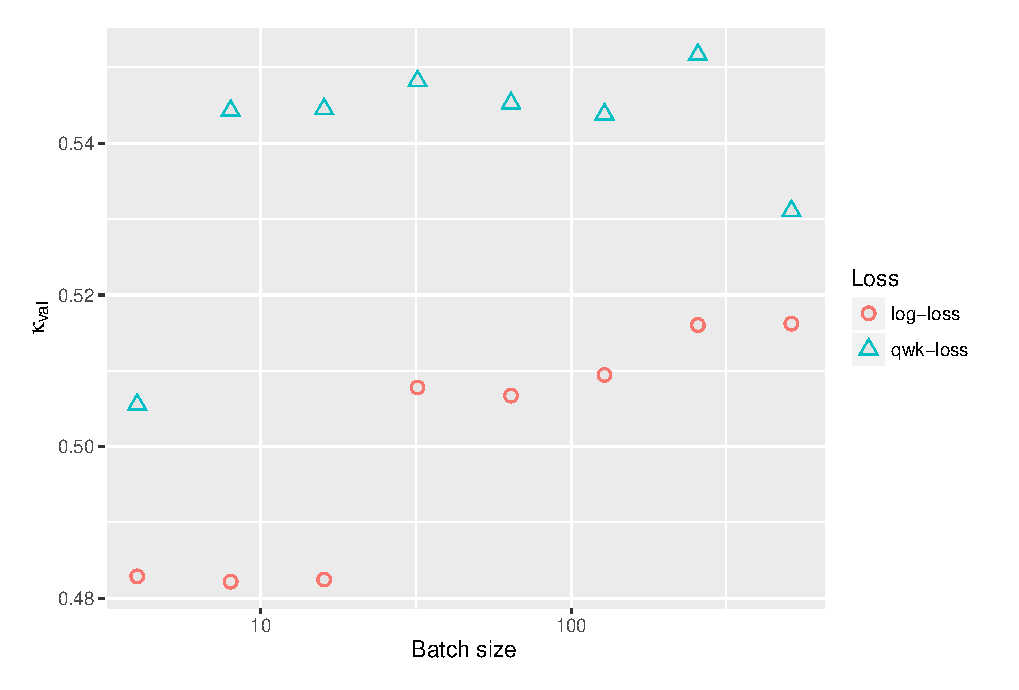
\includegraphics[width=\textwidth]{Figures/chapter_loss/crowdflower-results.eps}
	\caption[$QWK_{val}$ vs BS - Search results relevance use case]{$\kappa_{val}$ of the best model for every batch size  (case 1: search results relevance)}
	\label{loss:fig:crowdflower}
\end{figure}

\begin{table}[h!]
	\centering
	\scalebox{0.9}{ 
		\begin{tabular}{c|c|c|c|c|c|c}
			ID & BS & LR & $\kappa^{qwk\mbox{-}loss}_{val} 10^3$ & $Epoch^{qwk\mbox{-}loss}_{best}$ & $\kappa^{log\mbox{-}loss}_{val} 10^3$ & $Epoch^{log\mbox{-}loss}_{best}$\\
			\hline
			1 & \multirow{5}{*}{4}   & 1e-02 & 405 & 10 & 439 & 9\\
			2 &                      & 1e-03 & 485 & 6 & 476 & 6\\
			3 &                      & 5e-04 & \textbf{506} & 15 & \textbf{483} & 14\\
			4 &                      & 1e-04 & 503 & 19 & 467 & 3\\
			5 &                      & 1e-05 & 461 & 99 & 455 & 50\\
			\hline	
			6 & \multirow{5}{*}{8}   & 1e-02 & 450 & 13 & 444 & 6\\
			7 &                      & 1e-03 & \textbf{544} & 6 & \textbf{482} & 0\\
			8 &                      & 5e-04 & 524 & 9 & 475 & 18\\
			9 &                      & 1e-04 & 535 & 31 & 482 & 10\\
			10 &                     & 1e-05 & 445 & 99 & 479 & 50\\
			\hline	
			11 & \multirow{5}{*}{16} & 1e-02 & 504 & 18 & 425 & 3\\
			12 &                     & 1e-03 & 535 & 10 & 480 & 1\\
			13 &                     & 5e-04 & 543 & 11 & \textbf{480} & 1\\
			14 &                     & 1e-04 & \textbf{545} & 50 & 483 & 9\\
			15 &                     & 1e-05 & 395 & 99 & 479 & 86\\
			\hline	
			16 & \multirow{5}{*}{32} & 1e-02 & 515 & 12 & 436 & 2\\
			17 &                     & 1e-03 & 548 & 16 & 494 & 1\\
			18 &                     & 5e-04 & \textbf{548} & 17 & \textbf{508} & 4\\
			19 &                     & 1e-04 & 519 & 60 & 501 & 17\\
			20 &                     & 1e-05 & 385 & 99 & 485 & 99\\
			\hline	
			21 & \multirow{5}{*}{64} & 1e-02 & 520 & 10 & 473 & 8\\
			22 &                     & 1e-03 & 531 & 12 & 488 & 4\\
			23 &                     & 5e-04 & \textbf{545} & 37 & 506 & 9\\
			24 &                     & 1e-04 & 514 & 61 & \textbf{507} & 25\\
			25 &                     & 1e-05 & 377 & 99 & 400 & 99\\
			\hline	
			26 & \multirow{5}{*}{128} & 1e-02 & 513 & 4 & 479 & 5\\
			27 &                      & 1e-03 & \textbf{544} & 23 & 497 & 6\\
			28 &                      & 5e-04 & 527 & 31 & 499 & 8\\
			29 &                      & 1e-04 & 503 & 72 & \textbf{509} & 55\\
			30 &                      & 1e-05 & 317 & 99 &   0 & 0\\
			\hline	
			31 & \multirow{5}{*}{256} & 1e-02 & 510 & 8 & 490 & 1\\
			32 &                      & 1e-03 & \textbf{552} & 32 & \textbf{516} & 14\\
			33 &                      & 5e-04 & 490 & 21 & 507 & 24\\
			34 &                      & 1e-04 & 421 & 45 & 469 & 48\\
			35 &                      & 1e-05 & 189 & 99 & 61 & 34\\
			\hline	
			36 & \multirow{5}{*}{512} & 1e-02 & 512 & 18 & 488 & 7\\
			37 &                      & 1e-03 & \textbf{531} & 38 & \textbf{516} & 24\\
			38 &                      & 5e-04 & 509 & 64 & 493 & 27\\
			39 &                      & 1e-04 & 443 & 99 & 450 & 86\\
			40 &                      & 1e-05 & 15 & 4 & 41 & 43\\
			\hline			
		\end{tabular}
	}
	\caption[Search results relevance experiments]{List of all experiments for Case 1: Search results relevance}
	\label{loss:tab:crowdflower}
\end{table}

After the study, we check the performance of the best model trained with qwk-loss and log-loss, using the test set (i.e. against never seen before records) consisting on 256,735 records. The test of the best model trained with qwk-loss reports a $\kappa_{test} = 0.500 \pm 0.043$ (95\% confidence). The best model trained with log-loss achieves a kappa in the test set of $\kappa_{test} = 0.468 \pm 0.050$ (95\% confidence). The difference between the two models is about a 6\% increase of the value of $\kappa_{test}$ (see fig. \ref{loss:fig:retine-boxplot}).


\begin{figure}[!htb]
	\centering
	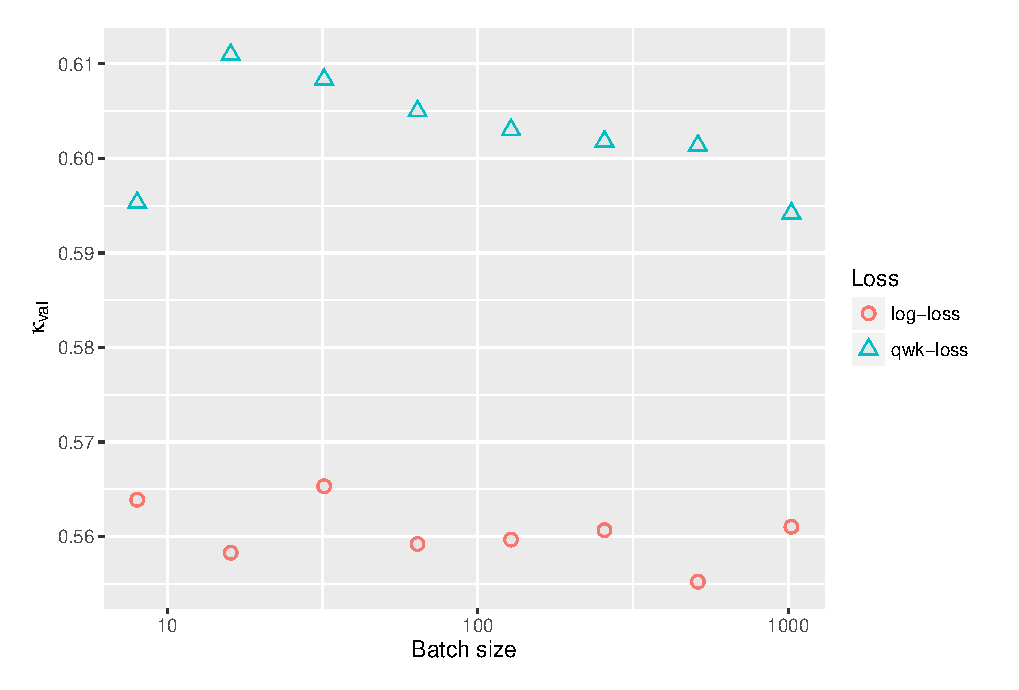
\includegraphics[width=\textwidth]{Figures/chapter_loss/prudential-results.eps}
	\caption[$QWK_{val}$ vs BS - Life insurance assessment use case]{$\kappa_{val}$ of the best model for every batch size (case 2: life insurance assessment)}
	\label{loss:fig:prudential}
\end{figure}

\begin{table}[h!]
	\centering
	\scalebox{0.9}{ 
		\begin{tabular}{c|c|c|c|c|c|c}
			ID & BS & LR & $\kappa^{qwk\mbox{-}loss}_{val} 10^3$ & $Epoch^{qwk\mbox{-}loss}_{best}$ & $\kappa^{log\mbox{-}loss}_{val} 10^3$ & $Epoch^{log\mbox{-}loss}_{best}$\\
			\hline
			1 & \multirow{5}{*}{8}  & 1e-02 & 412 & 0 & 564 & 5\\
			2 &                     & 1e-03 & 593 & 3 & 550 & 4\\
			3 &                     & 5e-04 & 592 & 8 & 556 & 2\\
			4 &                     & 1e-04 & \textbf{595} & 11 & \textbf{560} & 4\\
			5 &                     & 1e-05 & 588 & 20 & 556 & 27\\
			\hline
			6 & \multirow{5}{*}{16} & 1e-02 & 570 & 1 & 555 & 8\\
			7 &                     & 1e-03 & 605 & 5 & 550 & 4\\
			8 &                     & 5e-04 & \textbf{611} & 7 & \textbf{558} & 2\\
			9 &                     & 1e-04 & 605 & 7 & 558 & 9\\
			10 &                    & 1e-05 & 596 & 14 & 554 & 28\\
			\hline
			11 & \multirow{5}{*}{32} & 1e-02 & 587 & 0 & 560 & 1\\
			12 &                     & 1e-03 & 604 & 2 & \textbf{565} & 3\\
			13 &                     & 5e-04 & \textbf{608} & 2 & 552 & 4\\
			14 &                     & 1e-04 & 603 & 11 & 562 & 11\\
			15 &                     & 1e-05 & 598 & 24 & 545 & 44\\
			\hline
			16 & \multirow{5}{*}{64} & 1e-02 & 587 & 0 & 547 & 7\\
			17 &                     & 1e-03 & \textbf{605} & 3 & 557 & 5\\
			18 &                     & 5e-04 & 603 & 4 & \textbf{559} & 4\\
			19 &                     & 1e-04 & 600 & 5 & 557 & 8\\
			20 &                     & 1e-05 & 595 & 38 & 542 & 30\\
			\hline
			21 & \multirow{5}{*}{128} & 1e-02 & 592 & 2 & 554 & 4\\
			22 &                      & 1e-03 & 602 & 5 & \textbf{560} & 2\\
			23 &                      & 5e-04 & \textbf{603} & 4 & 556 & 8\\
			24 &                      & 1e-04 & 599 & 7 & 558 & 18\\
			25 &                      & 1e-05 & 567 & 48 & 537 & 45\\
			\hline
			26 & \multirow{5}{*}{256} & 1e-02 & 589 & 6 & 555 & 1\\
			27 &                      & 1e-03 & \textbf{602} & 3 & 555 & 2\\
			28 &                      & 5e-04 & 598 & 6 & 555 & 1\\
			29 &                      & 1e-04 & 592 & 6 & \textbf{561} & 20\\
			30 &                      & 1e-05 & 589 & 49 & 515 & 26\\
			\hline
			31 & \multirow{5}{*}{512} & 1e-02 & \textbf{601} & 16 & \textbf{555} & 1\\
			32 &                      & 1e-03 & 601 & 5 & 548 & 5\\
			33 &                      & 5e-04 & 598 & 3 & 554 & 9\\
			34 &                      & 1e-04 & 598 & 15 & 548 & 19\\
			35 &                      & 1e-05 & 563 & 49 & 523 & 48\\
			\hline
			36 & \multirow{5}{*}{1024} & 1e-02 & 594 & 4 & 549 & 3\\
			37 &                       & 1e-03 & 592 & 5 & \textbf{561} & 7\\
			38 &                       & 5e-04 & \textbf{594} & 5 & 554 & 12\\
			39 &                       & 1e-04 & 593 & 21 & 547 & 22\\
			40 &                       & 1e-05 & 472 & 49 & 470 & 49\\
			\hline			
		\end{tabular}
	}
	\caption[Life insurance assessment experiments]{List of experiments for Case 2: Life insurance assessment}
	\label{loss:tab:prudential}
\end{table}

\subsection{Case 2. Life insurance assessment}

In figure \ref{loss:fig:prudential}, the best results achieved on the training stage for every batch size and learning rate are shown. For each batch size, 5 LR values are tested. In bold we have the best $\kappa_{val}$ of each batch size. This are graphically displayed in fig. \ref{loss:fig:prudential}.
Next, the best parameters are chosen for the two models and the performance is evaluated using the test set, consisting on 19,765 records. The test of the best model trained with qwk-loss reports a $\kappa_{test} = 0.618 \pm 0.016$ (95\% confidence). In the case of the best model trained with log-loss the value of kappa in the test set is $\kappa_{test} = 0.562 \pm 0.018$ (95\% confidence). A significant difference between the two best models in the test set is found, with about a 10\% increase of the value of $\kappa_{test}$ (see fig. \ref{loss:fig:retine-boxplot}).


\subsection{Case 3. Diabetic retinopathy detection}

Table \ref{loss:tab:qwk_cv} shows the collection of all the conducted experiments where \emph{input} represents the size of the input layer, \emph{BS} the batch size used in the experiment, \emph{LR} the learning rate, \emph{$\kappa_{train}$} the maximum value of $\kappa$ achieved during training over the training set, \emph{$\kappa_{val}$} the maximum value of $\kappa$ achieved during training over the validation set, \emph{gap} the difference between $\kappa_{train}$ and $\kappa_{val}$, \emph{epoch} the epoch where the maximum value of $\kappa_{val}$ is achieved and finally \emph{updates} the number of parameters updates required to achieve the maximum value of $\kappa_{val}$.


% Aquí taula 4
\begin{table}[h!]
	\centering
	\scalebox{0.85}{
	\resizebox{\columnwidth}{!}{ 
		\begin{tabular}{c|c|c|c|c|c|c|c|c}
			Input & BS & Loss & LR	& $\kappa_{train} 10^3$ & $\kappa_{val} 10^3$ & Gap & Epoch & Updates $10^{-3}$\\	
			\hline
			\multirow{32}{*}{128} & \multirow{6}{*}{5} & \multirow{3}{*}{log} & $10^{-5}$ & 771 & 418 & 353 & 78 & 1560\\
			& & & $10^{-4}$ & 851 & \textbf{491} & 360 & 73 & 1460\\
			& & & $10^{-3}$ & 676 & 418 & 258 & 29 & 580\\\cline{3-9}
			& & \multirow{3}{*}{qwk} & $5 \times 10^{-5}$ & 545 & 402 & 143 & 50 & 1000\\
			& & & $10^{-5}$ & 646 & 439 & 207 & 70 & 1400\\
			& & & $10^{-4}$ & 497 & 326 & 171 & 31 & 620\\\cline{2-9}
			&\multirow{6}{*}{10} & \multirow{3}{*}{log} & $10^{-5}$ & 797 & 397 & 400 & 82 & 820\\
			& & & $10^{-4}$ & 874 & 455 & 419 & 81 & 810\\
			& & & $10^{-3}$ & 514 & 336 & 178 & 57 & 570\\\cline{3-9}
			& & \multirow{3}{*}{qwk} &  $10^{-5}$ & 774 & 476 & 298 & 82 & 820\\
			& & & $10^{-4}$ & 755 & 503 & 252 & 84 & 840\\
			& & & $10^{-3}$ & 596 & 289 & 307 & 95 & 950\\\cline{2-9}		
			& \multirow{6}{*}{15} & \multirow{3}{*}{log} & $10^{-5}$ & 803 & 368 & 435 & 79 & 527\\
			& & & $10^{-4}$ & 899 & 458 & 441 & 95 & 633\\
			& & & $10^{-3}$ & 868 & 447 & 421 & 80 & 533\\\cline{3-9}
			& & \multirow{3}{*}{qwk} & $5\times10^{-5}$ & 715 & 491 & 224 & 77 & 513\\
			& & & $10^{-4}$ & 800 & 526 & 274 & 77 & 513\\
			& & & $5\times10^{-4}$ & 823 & 523 & 300 & 72 & 480\\\cline{2-9}
			& \multirow{2}{*}{20} & log & $10^{-4}$ & 896 & 474 & 422 & 79 & 395\\\cline{3-9}
			& & qwk & $10^{-4}$ & 835 & \textbf{537} & 298 & 93 & 465\\\cline{2-9}
			& \multirow{6}{*}{25} & \multirow{3}{*}{log} & $10^{-5}$ & 821 & 315 & 506 & 96 & 384\\
			& & & $10^{-4}$ & 913 & 453 & 460 & 93 & 372\\
			& & & $10^{-3}$ & 849 & 382 & 467 & 70 & 280\\\cline{3-9}
			& & \multirow{3}{*}{qwk} & $10^{-5}$ & 808 & 423 & 385 & 95 & 380\\
			& & & $10^{-4}$ & 824 & 499 & 325 & 65 & 260\\
			& & & $10^{-3}$ & 655 & 447 & 208 & 80 & 320\\\cline{2-9}
			& \multirow{2}{*}{100} & \multirow{3}{*}{log} & $10^{-4}$ & 929 & 377 & 552 & 98 & 98\\
			& & & $10^{-3}$ & 947 & 444 & 503 & 99 & 99\\
			& & & $10^{-2}$ & 842 & 412 & 430 & 67 & 67\\\cline{3-9}
			& & \multirow{3}{*}{qwk} & $10^{-4}$ & 879 & 450 & 429 & 93 & 93\\
			& & & $10^{-3}$ & 798 & 455 & 343 & 71 & 713\\
			& & & $10^{-2}$ & - & - & - & - & -\\
			\hline	
			\multirow{10}{*}{256} & \multirow{2}{*}{5} & \multirow{1}{*}{log} & $10^{-4}$ & 871 & \textbf{571} & 300 & 52 & 1040\\\cline{3-9}
			& & \multirow{1}{*}{qwk} & $10^{-4}$ & 605 & 433 & 172 & 15 & 300\\\cline{2-9}
			&\multirow{2}{*}{10} & \multirow{1}{*}{log} & $10^{-4}$ & 903 & 566  & 337 & 75 & 750\\\cline{3-9}
			& & \multirow{1}{*}{qwk} & $10^{-4}$ & 832 & 616 & 216 & 70 & 700\\\cline{2-9}		
			& \multirow{2}{*}{15} & \multirow{1}{*}{log} & $10^{-4}$ & 925 & 556 & 369 & 98 & 653\\\cline{3-9}
			& & \multirow{1}{*}{qwk} & $10^{-4}$ & 878 & \textbf{622} & 256 & 93 & 620\\\cline{2-9}
			& \multirow{2}{*}{20} & \multirow{1}{*}{log} & $10^{-4}$ & 923 & 525 & 398 & 97 & 485\\\cline{3-9}
			& & \multirow{1}{*}{qwk} & $10^{-4}$ & 891 & 618 & 273 & 97 & 485 \\\cline{2-9}		
			& \multirow{2}{*}{30} & \multirow{1}{*}{log} & $10^{-4}$ & 925 & 514 & 411 & 93 & 310\\\cline{3-9}
			& & \multirow{1}{*}{qwk} & $10^{-4}$ & 900 & 586 & 314 & 98 & 327\\\cline{2-9}
			& \multirow{2}{*}{40} & \multirow{1}{*}{log} & $10^{-4}$ & 922 & 464 & 458 & 93 & 233\\\cline{3-9}
			& & \multirow{1}{*}{qwk} & $10^{-4}$ & 894 & 592 & 302 & 78 & 195\\\cline{2-9}
			\hline					
			\multirow{2}{*}{384} & \multirow{1}{*}{5} & \multirow{1}{*}{log} & $10^{-4}$ & 863 & \textbf{641} & 222 & 38 & 760\\\cline{2-9}
			& \multirow{1}{*}{15} & \multirow{1}{*}{qwk} & $10^{-4}$ & 889 & \textbf{698} & 191 & 93 & 620 \\\cline{2-9}
			\hline					
			\multirow{4}{*}{512} & \multirow{1}{*}{5} & \multirow{1}{*}{log} & $10^{-4}$ & 980 & \textbf{681} & 299 & 88 & 1760\\\cline{2-9}
			& \multirow{2}{*}{15} & \multirow{1}{*}{log} & $10^{-4}$ & 978 & 668 & 310 &  94 & 626\\\cline{3-9}
			&  & \multirow{1}{*}{qwk} & $10^{-4}$ & 884 & \textbf{717} & 167 & 86 & 573 \\\cline{2-9}
			& \multirow{1}{*}{20} & \multirow{1}{*}{qwk} & $10^{-4}$ & 903 & 701 & 202 & 89 & 445\\\cline{3-9}			
			\hline
		\end{tabular}
	}
	}
	\caption[DR detection experiments]{List of experiments for Case 3: DR detection}
	\label{loss:tab:qwk_cv}
\end{table}

We can see that for every input size the maximum value achieved over the training set optimizing qwk-loss is always higher than the maximum value achieved optimizing log-loss (bold values). The gaps between both training and validation are also lower in the case of qwk-loss indicating a lower overfitting of the training data. We see that qwk-loss consistently reports better results than log-loss except for very low values of BS. In those cases, the qwk-loss performs worse than log-loss, but even in those cases the maximum value achieved by log-loss is lower than the best value of qwk-loss for the same model over the whole set of experiments.

In figure \ref{loss:fig:best} we show a graphical representation of the maximum value of $\kappa_{val}$ for the different configurations. We can see that directly optimizing qwk-loss gives consistently better results than optimizing log-loss. Only in the case of very small batch sizes (for this application case, BS = 5) log-loss performs better than qwk-loss. This is probably due to the fact that qwk-loss uses a normalization term in the denominator that with not big enough batch sizes could cause instabilities in the gradient that affect the performance. In any case, even in those cases the results obtained with the log-loss are worse that the best achieved using the qwk-loss configuration.

\begin{figure}[!htb]
	\centering
	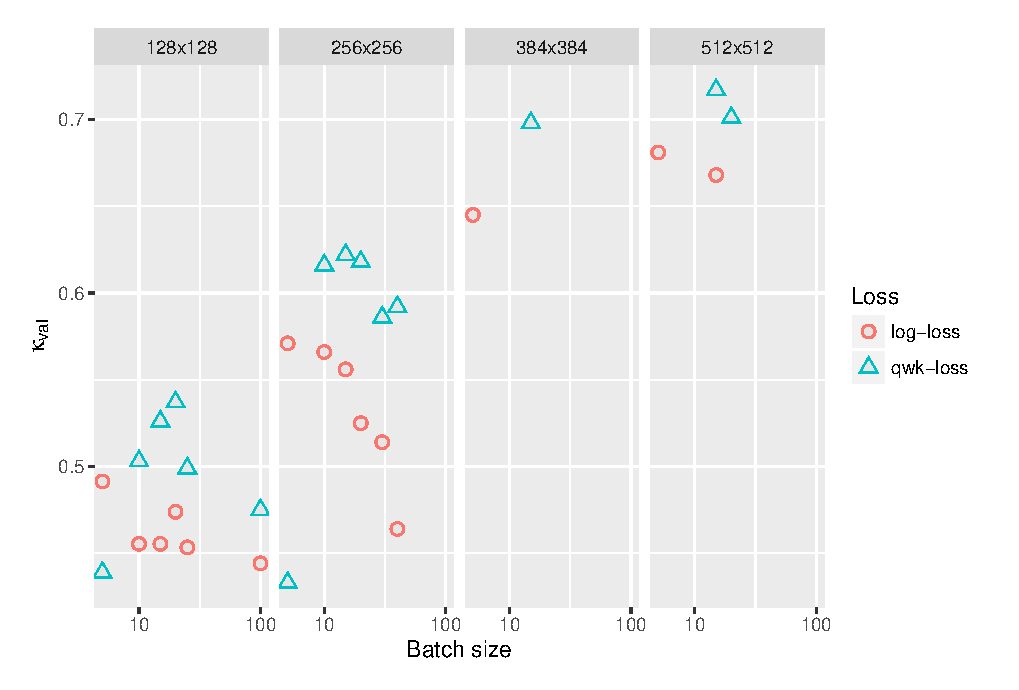
\includegraphics[width=\textwidth]{Figures/chapter_loss/retine-results.eps}
	\caption[$QWK_{val}$ vs BS - Diabetic Retinopathy detection use case]{$\kappa_{val}$ achieved for the DR detection use case in every experiment in function of the batch size and the loss function used}
	\label{loss:fig:best}
\end{figure}

The optimal batch size for solving this DR classification is of 5 in the case of using the log-loss and 15 in the case of the qwk-loss. For greater values of this hyper-parameter, the increase in precision of the calculation of the gradient does not report any advantage in the optimization. In the case of the log-loss a lower precision in the calculation of the gradient works better. It could probably be due to the fact that this imprecision in the calculation increases the stochasticity of the optimization and due to the fact that we are not optimizing directly the metrics index. This makes possible to explore adjacent zones that could work better for improving the metrics index than the ones that specifically improve the log-loss. Additionally, although smaller batch sizes give worse approximations of the gradient, the number of updates per epoch of the parameters of the model is greater. This seems to be an advantage in this case.

After all this study, we check the performance of the best model trained with qwk and log losses against the \emph{never seen before} 53,576 image test set. The test of the best model trained with qwk-loss reports a $\kappa_{test} = 0.740 \pm 0.006$ (95\% confidence). In the case of the same model trained with log-loss the value of $\kappa_{test} = 0.686 \pm 0.008$ (95\% confidence). The difference between the two best models in the test set is of more than a 7\% increase of the value of $\kappa$. (see case 3 in fig. \ref{loss:fig:retine-boxplot})

Fig. \ref{loss:fig:confusion-retine} helps to understand the difference between the performance of the optimized loss functions. This figure displays the histograms of the predicted classes for every true class. It can seen how the predicted histograms of the log-loss trained model are more scattered than the ones of the qwk-loss trained model. In those cases where there is a discrepancy between the real value and the predicted one, the model trained with the qwk-loss assign a category that are closer to the true category than the ones predicted by the log-loss trained model. This can be seen specially in the central category T2, where the distribution of qwk-loss model is concentrated in categories 1, 2 and 3 (with around 30\% each), while in the log-loss model, there are 25\% observations classified into class 0 as well as 10\% into class 4. This is of great importance when the classification is related with medical diagnosis. For a patient having severe retinopathy (class 4) it is better to be classified having a moderate or a proliferative one (closer classes) than to be classified as having a mild or as not having any retinopathy at all.

\begin{figure}[!htb]
	\centering
	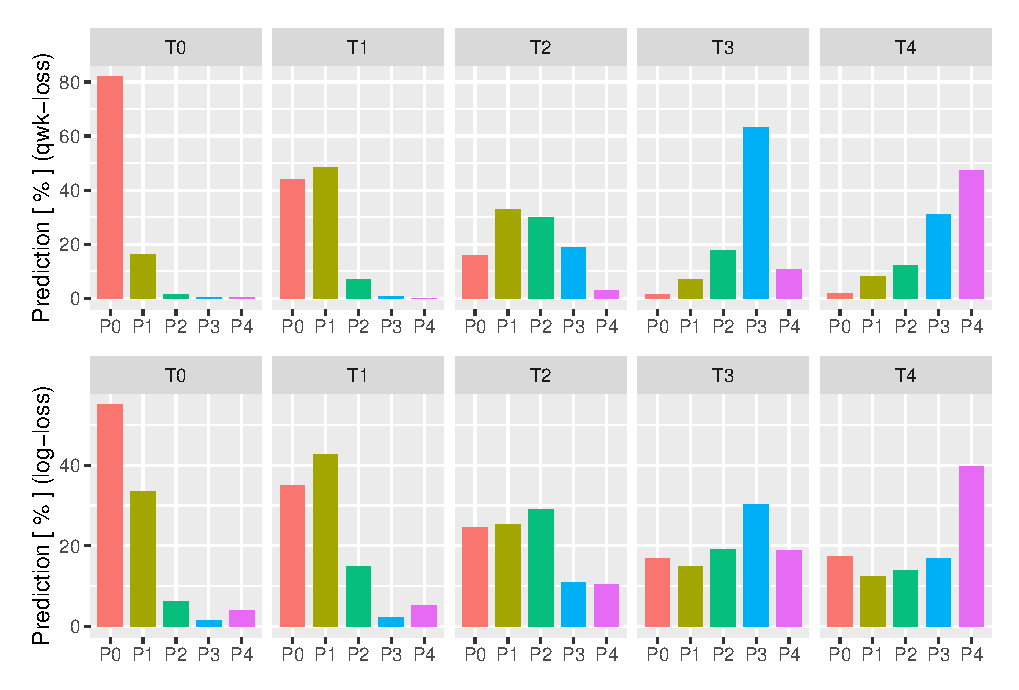
\includegraphics[width=\textwidth]{Figures/chapter_loss/confusion-retine.eps}
	\caption[Histograms of DR prediction (qwk-loss vs log-loss)]{Histograms of the predicted classes for every real class over the test set for the best qwk-loss (above) and log-loss (below) trained models in the DR multi-class classification use case}
	\label{loss:fig:confusion-retine}
\end{figure}

\begin{table}[h!]
	\centering
	\scalebox{0.85}{ 
		\begin{tabular}{c|c|c|c|c|c|c|c}
			Input & \specialcell{Total\\Layers} & \specialcell[t]{Feature\\Layers} & \specialcell[t]{Classific.\\Layers} &  \specialcell[t]{Params\\$10^{-6}$} & $\kappa_{val}^{qwk\mbox{-}loss}$ & $\kappa_{val}^{log\mbox{-}loss}$ & $\Delta$\\
			\hline
			128x128 & 12 & 10 & 1 & 1.16 & 0.537 & 0.491 & 9.3 \%\\
			256x256 & 14 & 12 & 1 & 1.44 & 0.622 & 0.571 & 8.9 \%\\
			384x384 & 14 & 12 & 1 & 1.77 & 0.698 & 0.663 & 5.3 \%\\
			512x512 & 14 & 12 & 1 & 11.3 & 0.717 & 0.681 & 5.3 \%\\
			\hline
		\end{tabular}
	}
\caption{Summary of the difference in performance between qwk-loss and log-loss trained models in function of input size for the DR detection case}
\label{loss:tab:models}
\end{table}

\subsection{Overall discussion on the performance improvement}

In this section, the quality of the classification with the testing datasets is analyzed, although a brief comment has been made before on each case study.
Figure \ref{loss:fig:retine-boxplot} shows the $\kappa$ index obtained on the testing data for the three case studies with the best model of every loss function. With this figure we can check if the difference between the two optimization techniques is statistically significant or not.
Improvement is clear for Case 2 and Case 3. Case 1 also has almost non-overlapping boxplots
but the $\kappa_{test}$ value achieved is more similar in the two models. However, in this case study the neural network used was the simplest one, thus the influence of the loss function in the final model is less. Improvement achieved with qwk-loss optimization is, thus, clear and supports the initial hypothesis of this research work.

\begin{figure}[!htb]
	\centering
	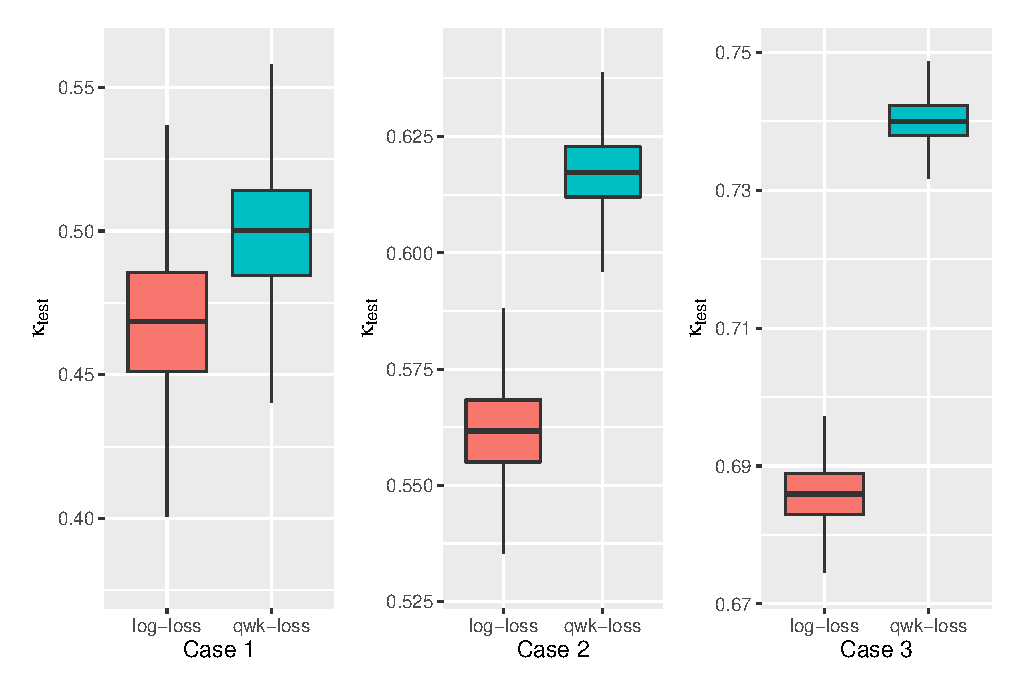
\includegraphics[width=\textwidth]{Figures/chapter_loss/boxplots.eps}
	\caption[QWK use cases confidence intervals]{QWK confidence intervals for the log and qwk best models for the three studied cases}
	\label{loss:fig:retine-boxplot}
\end{figure}

\section{Conclusions}\label{loss:conc}

We presented a new loss function for training deep learning models in ordinal classification problems based on the optimization of the weighted kappa index. In contrast to the logarithmic loss that uses a uniform prior over the set of classes, this new loss function defines a penalization over the discrepancy that is proportional to a power of the distance (quadratically in the case of $\kappa$) that allows to encode the prior known information about the predefined ordering of the classes. 

We checked the performance of this new loss function with three different real-world case studies with diverse types of input data: textual in the first, categorical and numerical in the second and images in the third. Moreover, each case study was solved using decision models of increasing level of complexity: a linear classifier in the first, a multilayer perceptron in the second and a deep convolutional neural network in the third. 

The results presented in this chapter show that with the direct optimization of the $\kappa$ index consistently better generalization results can be achieved than with the standard use of the logarithmic loss. Log-loss has to learn the predefined ordering of the classes from data and this seems to be a disadvantage. Results showed that, depending on the use case, between 6-10\% of improvement of $\kappa$ scores can be obtained from the direct optimization of the function.

This is a significant improvement that may be worth in many domains, such as the one of medical diagnosis, since an accurate detection of the level of severity of a disease usually has great influence on the treatment prescription and the possibility of minimizing bad consequences of the illness.

One minor drawback of the new loss is its low performance with very small batch sizes in the image classification study. The experiments show that for the retinopathy classification problem with batch sizes of 5, the performance of the function is lower than using the logarithmic loss. This parameter is for sure problem dependent and has to be taken into account as an important parameter to check in other image classification tasks that use a deep neural network.

% Chapter Template

\chapter{Enhanced Models} % Main chapter title

\label{Chapter:Ordinal_Regression} % Change X to a consecutive number; for referencing this chapter elsewhere, use \ref{ChapterX}

In this chapter we present a part of the work published in \citep{de2017deep}. Concretely, the optimized classification model for DR disease grading. The model presented here has a statistically proven ophthalmologist level performance, reaching a inter-rating agreement in never-seen-before Messidor dataset of $QWK = 0.83$, with a unique evaluation and no ensembling. 

%----------------------------------------------------------------------------------------
%	SECTION 1
%----------------------------------------------------------------------------------------

\section{Introduction}

Deep Learning (DL) methods \citep{nature-deep-learning}, \citep{888} have been extensively used in the last years for many automatic classification tasks. For the case of image classification, the usual procedure consists on extracting the important features using a set of convolutional layers and, after that, make a final classification with these features using a set of fully connected layers. At the end, a soft-max output layer gives the predicted output probabilities of belonging to the classes predefined in the model. During training, model parameters are changed using a gradient-based optimization algorithm, which minimizes a predefined loss function.\citep{Goodfellow-et-al-2016} 

Once the classifier has been trained (i.e. model layer parameters have been fixed), the quality of the classification output is compared against the correct "true" values stored on a labeled dataset. This data is considered as the gold standard, ideally coming from the consensus of the knowledge of a committee of human experts.

This mapping allows the classification of multi-dimensional objects into a small number of categories. The model is composed by many neurons that are organized in layers and blocks of layers, piled together in a hierarchical way. Every neuron receives the input from a predefined set of neurons. In addition, every connection has a parameter that corresponds to the weight of the relation. 

The function of every neuron is to make a transformation of the received inputs into a calculated output value. For each incoming connection, a weight is multiplied by the input value and the aggregation over all inputs is fed to an activation function that calculates the neuron output. Parameters are usually optimized using a stochastic gradient descent algorithm that minimizes a predefined loss function. Network parameters are updated after back-propagating the loss function gradients through the network. These hierarchical models are able to learn multiple levels of representation that correspond to different levels of abstraction, which enables the representation of complex concepts in a compressed way \citep{Bengio:2013:RLR:2498740.2498889}, \citep{bengio-2009}.

The first successful convolutional neural network (CNN) published \citep{LeCun:98} was designed for hand-written digit recognition. This early CNN implementation used a combination of convolution, pooling and non-linearity that has been the key feature of DL until now. It used convolutions for extracting spatial features, sub-sampling for reducing maps size, a non-linearity in the form of tanh or sigmoids, and a fully connected multi-layer neural network as final classifier.  Network parameters were all learned using an end-to-end optimization algorithm using stochastic gradient descent. One of the first successful implementations using GPUs was published in \citep{ciresan80deep} where they successfully trained a neural network with 9 layers, also for handwritten digit recognition. The DL breakthrough took place with the publication of \citep{NIPS2012_4824} where, for the first time, a CNN won the Imagenet\citep{imagenet_cvpr09} classification competition by a large margin. The network, named AlexNet, introduced a set of innovative techniques like data augmentation, the use of rectified linear units (ReLUs) as non-linearities, the use of dropout for avoiding overfitting, overlapping max-pooling avoiding the averaging effects of avg-pooling and the use of GPUs for speeding up the training time. This paper proved experimentally that CNNs were able to solve complex tasks. From the publication of this paper many improvements where published, like \citep{sermanet2014overfeat} with the introduction of Overfeat, a network derivation of AlexNet where they proposed learning bounding boxes, which later gave rise to many other papers on the same topic. In \citep{vggnet}, VGG networks where presented. It was the first time that small 3x3 convolution filters where used and combined as a sequence of convolutions. The previous big filters of 9x9 and 11x11 present in AlexNet started to become smaller. The great advantage of VGG network was the insight of stacking 3x3 convolutions as a substitution of large filters. These ideas were used in the design of posterior networks like ResNet and Inception. GoogleNet\citep{googlenet} and Inception \citep{szegedy2016rethinking} were the first attempts to reduce the size of big networks. DL was becoming very useful for categorization of images and video frames, but its main concern was its low efficiency in size and computation. Inception module used a parallel calculation of 1x1, 3x3 and 5x5 convolutions significantly reducing the number of operations required by networks like AlexNet and VGG. Bottleneck layers (1x1 convolutions) where used before the calculation of bigger size convolutions for reducing the number of input filters, reducing in this way the computational costs without losing generality. So, 1x1 convolutions have been proven to achieve state-of-the-art results in Imagenet classification tasks. The reason of this success is that input features are correlated, being removed by combining them appropriately with the 1x1 convolutions. Then, after convolution with a smaller number of features, they can be expanded again into a meaningful combination for the next layer. Another revolution came with the introduction of residual networks in \citep{he2016deep}. These networks used a combination of 3x3 convolutional layers with a by-pass of the input every two layers that was summed up to the output. The introduction of such bypass improved the gradient propagation through the network allowing the use of deeper networks and improving the classification capabilities. In \citep{szegedy2017inception}, a modified version of Inception networks called InceptionResNet was published to introduce this idea to such networks. Residual blocks allowed the reduction of training time, not improving significantly the classification performance. 
%\vspace{1cm} % just to get a page break. Remove if not required

DL models have been also successfully applied  in many medical classification tasks. In \citep{esteva2017dermatologist} a DL classifier was designed achieving dermatologist-level accuracy for skin cancer detection. In \citep{wentao2018deeplung} a 3D CNN for automated pulmonary nodule detection and classification was built. In \citep{wang2018classification} a CNN Alzheimer's disease classifier with high performance was also described. In \citep{doi:10.1001/jama.2016.17216} the authors presented a DR classifier with better performance than human experts in the detection of the most severe cases of the disease.

\section{Related work}\label{class2:sec:related}

Many deep learning classifiers for DR have been published in the last years. In \citep{delatorre2017} a DL classifier was published for the prediction of the different disease grades. This model was trained using the public available EyePACS dataset. The training set had 35,126 images and the test set 53,576. The quadratic weighted kappa (QWK) evaluation metric \citep{cohen1968weighted} was close to the reported by human experts in the test set using a unique DL model without ensembling. 

In \citep{doi:10.1001/jama.2016.17216} a binary DL classifier was published for the detection of the most severe cases of DR (grouping classes 0 and 1 of DR on one side, and classes 2, 3 and 4 on another). This model was trained using an extended version of the EyePACS dataset mentioned before with a total of 128,175 images and improving the proper tagging of the images using a set of 3 to 7 experts chosen from a panel of 54 US expert ophthalmologists. This model surpassed the human expert capabilities, reaching approximately a performance of 97\% in sensitivity and 93.5\% in specificity in test sets of about 10,000 images. The strength of this model was its ability to predict the more severe cases with a sensitivity and specificity greater than human experts. The drawback, as many DL based models, is its lack of interpretability. The model acts like a \emph{intuition machine} with a highly statistical confidence but lacking an interpretation of the rationale behind the decisions, making difficult to the experts to have clues to improve the diagnostics.

\section{Classification model for DR} \label{class2:sec:class}

\subsection{Data}
\label{class2:sec:data}

We use the EyePACS dataset presented in chapter \ref{Chapter:Background}. The dataset is split into two disjoint sets containing eye images of different patients, one for training and the other for testing.

The training set contains a total of $75,650$ images; $55,796$ of class 0, $5,259$ of class 1, $11,192$ of class 2, $1,805$ of class 3 and $1,598$ of class 4. The validation set used for hyper-parameter optimization has $3,000$ images; $2,150$ of class 0, $209$ of class 1, $490$ of class 2, $61$ of class 3 and $90$ of class 4. 

The test set contains a total of $10,000$ images of patients not present in training set; $7,363$ of class 0, $731$ of class 1, $1,461$ of class 2, $220$ of class 3 and $225$ of class 4. 

This dataset is not so rich and well tagged as the used in \citep{doi:10.1001/jama.2016.17216} but allows to train models near human expertise that are useful to show the purposes of our work, which is not only a good performance of the classification results but mainly to provide tools for interpretability of the final classification of each patient.

\subsection{Construction of the classifier}

The model calculates the probability $P(\mathcal{C} | \mathcal{I})$, being $\mathcal{C}$ one of the possible output classes and $\mathcal{I}$ the retina image. Using as a last layer a $SoftMax$ function over the values after the last linear combination of features. This probability is calculated as $P(\mathcal{C} | \mathcal{I}) = \frac{\me^{S_{i}}}{\sum_{j=1}^{C} \me^{S_{j}}}$. Let us call $S_{C}$ the score of class $C$, being $S_C$ the final value of each output neuron before applying the $Softmax$. $Softmax$ function is required for calculating the probability of every class, but in case of being interested only on $argmax(Softmax)$, we do not need evaluate $Softmax$ because $argmax(S_i) = argmax(Softmax(S_i))$. Thus, we skip $Softmax$ from the interpretation analysis.

\subsubsection{Design guidelines for DR classification} \label{class_guidelines}

Up to now, the design of deep neural network models is mainly driven  by experience. Nowadays it is still more an art than a science and lacks a systematic way for designing the best architecture for solving a problem. In previous works (see \citep{jdelatorre2016} and \citep{delatorre2017}), we have tested different kinds of architectures for DR classification. Using the previous experience in such works we report here a set of guidelines that have been used to build the proposed classification model for DR. These design principles for DR classification can be summarized into: use an optimal image resolution, use all the image information available, use a fully CNN, use small convolutions, adapt the combination of convolution sizes and number of layers to have a final RF as similar as possible to the image size, use ReLU as activation function, use batch normalization in every layer, use QWK as a loss function, use a efficient number of features and use a linear classifier as the last layer.

\paragraph{Use an optimal image resolution} On the one hand, image input size has a great importance in the classification results. For this problem, other papers like \citep{jdelatorre2016} have shown that better results can be achieved with retina diameters of 512 pixels than with 384, 256 or 128 pixels. Some tests done using densities larger than 512 pixel/diameter seem to not improve significantly the classification rates. On the other hand, the hardware of calculation devices fix a limitation on the available resources. Input image size has a great impact on the memory and calculation time required for the training and test of the deep neural network models. For this present work, we tested models of 128, 256, 384, 512, 640, 724, 768 and 892 pixels of retina diameter. With this dataset, diameters greater than 640 does not seem to report better results. The optimal size is a retina diameter equal to 640 pixels. This is the one used for the results shown in this chapter.

\paragraph{Use all the available image information} In previous studies published in \citep{jdelatorre2016}, due to hardware limitations, the classification models were designed using limited input information, using only part of the available input, requiring ensembling solutions to combine the results from evaluating different parts of the same retina. A 512x512 input image model was used with a random selection of a rotated square (diagonal equal to the retina diameter). In this way only a 64\% of the retina information available was used in the classification prediction. On test time, five rotated versions of the input where averaged in order to get a better evaluation result. In this chapter, we use a network that receives all the input information available not requiring ensembling on test time. Only background located further from the diameter is removed.

\paragraph{Use a fully convolutional neural network} CNNs are computationally more efficient than fully connected ones. CNNs are ideal for exploiting the typical high local pixel correlations present in images.

\paragraph{Use small size convolutions} Spatial convolutions are very expensive in memory and time requirements, growing both quadratically with kernel size. Papers \citep{vggnet}, \citep{he2016deep},  \citep{szegedy2016rethinking} proved experimentally that stacking small convolution layers and increasing depth is possible to obtain better results than using convolutions of bigger size with less depth. In \citep{eldan2016power} and \citep{cohen2016expressive} theoretical studies proved also that model expressiveness grows exponentially with depth. In our chapter, we follow a similar approach to the one used in \citep{vggnet} using exclusively 3x3 convolutions in every feature layer. Even convolution sizes are discarded due to its asymmetry when used with zero padding.

\begin{figure}[ht!]
	\centering
	\includegraphics[width=0.50\textwidth]{Figures/chapter_classification/figures/receptive_field_640.pdf}
	\caption{Model RF growth}
	\label{class2:fig:rf_graph}
\end{figure}

\paragraph{Adapt convolution sizes and number of layers to get a RF as similar as possible to the image size} One important aspect of CNNs is the RF size. RF defines the theoretical space covered by a convolution in the input-space. The ideal case is having a RF in the last layer equal to the image size, because in such a way we are sure that all the information available is used. RFs greater than image size are inefficient, for this reason sometimes can be necessary to slightly modify the convolution sizes of some layer to get the desired one. Figure \ref{class2:fig:rf_graph} shows the RF growth of our model.

\paragraph{Use rectified linear unit (ReLU) as activation function} ReLU is a computationally efficient activation function that is very suitable to be used with very deep CNNs\citep{Dahl2013}. We have tested other activation functions such as LeakyReLU, ELU and SeLU reporting similar and even worse results, introducing complexity to the model without adding any significant advantage to the final result.

\paragraph{Use batch normalization in every layer} Batch normalization \citep{batch-norm} stabilize the training and accelerates convergence. In this application there is a great difference between using batch normalization or not. To the point that not using it makes very difficult or even impossible the training.

\paragraph{Use QWK as a loss function} For multi-class classification the standardized loss function to use is the logarithmic loss \citep{Goodfellow-et-al-2016}. In \citep{delatorre2017} it is shown that for ordinal regression problems, where not only a multi-class classification is taking place but also it is possible to establish a sorting of the classes based on some hidden underlying causes, QWK-loss can also be used with better results. The properties of this function as a loss function have been widely studied in \citep{delatorre2017}. The difference in performance of the final results is very high. Optimizing directly QWK allows achieving better classification results.

\paragraph{Use a linear classifier as a last layer} For simplicity and interpretability, we expect the model to disentangle completely the features required for the classification. Final classification is required to be done using a linear combination of last layer features.

\begin{figure}[ht!]
	\centering
	\includegraphics[width=0.50\textwidth]{Figures/chapter_classification/figures/PCA_feature_space.pdf}
	\caption{Feature space cummulative PCA variance of training set}
	\label{class2:fig:pca_graph}
\end{figure}

\paragraph{Use a efficient number of features} With infinitely number of resources we can use a big network. In our project we have limited device resources. In addition, we would like to be able to implement the result in devices with low resources too. Having this in mind, we tested networks of different sizes. In order to check the redundancy of information, we made a principal component analysis (PCA) in the feature space of the last layer, arriving to the conclusion that about 32 of the features explain 98.3 \% and 48 features, 99.997\% of the total variance. We studied different configurations using different number of features from 512 to 32. Values of 32 showed a reduction in performance that increased when using 64 features. Higher number of features did not improve the results. In figure \ref{class2:fig:pca_graph} we show the variance explained by the 64 feature vector space.

\subsubsection{Classification model description}

Following the given guidelines, our model uses a 3x640x640 input image obtained from a minimal preprocessing step, where only the external background borders are trimmed and later resized to the required input size. Figure \ref{class2:fig:drmodel} shows a block diagram of the model. It is a CNN with 391,325 parameters, divided in 17 layers. Layers are divided into two groups: the feature extractor and the classifier. The feature extraction has 7 blocks of 2 layers. Every layer is a stack of a 3x3 convolution with stride 1x1 and padding 1x1 followed by a batch normalization and a ReLU activation function. Between every block a 2x2 max-pooling operation of stride 2x2 is applied. After the 7 blocks of feature extraction, the RF of the network has grown till reaching 637x637, that is approximately equal to the input size 640x640 (see fig \ref{class2:fig:rf_graph} to see the RF of every layer). Afterwards, the classification phase takes place using a 2x2 convolution. A 4x4 average-pooling reduces the dimensionality to get a final 64 feature vector that are linearly combined to obtain the output scores of every class. A soft-max function allows the conversion of scores to probabilities to feed the values to the proper cost function during the optimization process. The feature extractor has 16 filters in the first block, 32 in the second and 64 in all the other.

\subsection{Training procedure}

As presented in section \ref{class2:sec:data}, the training set training set has 75,650 images and the validation set used for hyper-parameter selection 3,000. Notice that the image set is highly imbalanced. In order to facilitate the learning, the training set is artificially equalized using data augmentation techniques \citep{Krizhevsky:2012} based on $0-180^{\circ}$ random rotation, X and Y mirroring and contrast\&brightness random sampling.

A random initialization based in the Kaiming\&He approach \citep{kaiming} is used. All models are optimized using a batch based first order optimization algorithm called Adam \citep{DBLP:journals/corr/KingmaB14}. The loss function used for optimizing the model is the QWK-loss function, with a batch size of $15$ and a learning rate of $3x10^{-4}$ \citep{delatorre2017}. For every batch, the images are chosen randomly from the training set, with repetition. 

After network training, a linear classifier formed by the combination of the 128 features of the two eyes of the patient is trained. In this way is possible to increase further the prediction performance of the model using all the information available of the patient.

\begin{figure}[ht!]
	\centering
	\scalebox{0.9}{
		\begin{subfigure}[b]{.31\textwidth}
			\centering
			\includegraphics[width=\textwidth]{Figures/chapter_classification/figures/model640.pdf}
			%\caption{Full classification stack}	
		\end{subfigure}
		\hfill    
		\begin{subfigure}[b]{.30\textwidth}
			\centering
			\includegraphics[width=\textwidth]{Figures/chapter_classification/figures/modelblock.pdf}\\
			\vspace{2cm}
			\includegraphics[width=\textwidth]{Figures/chapter_classification/figures/modellayer.pdf}\\
			\vspace{2cm}
			%\caption{Block and layer constituents}
		\end{subfigure}
	}
	\hfill 
	\caption[Prediction model]{Prediction model of 391,325 trainable parameters (located in blue blocks).}  
	\label{class2:fig:drmodel} 
\end{figure}

\section{Results}\label{class2:sec:results}

The model is trained for 300 epochs, reaching a QWK value of $0.814$ on the validation set. The value achieved in the testing set (with images not used in the training) of 10,000 images is of $0.801$. Using a linear classifier for combining the features of both eyes $QWK_{test}$, we can reach a QWK value of $0.844$. Expert ophthalmologist report QWK inter-rating agreement values close to $0.80$. 

If we consider a binary classification with two categories, one for severe cases of DR (grouping classes 2, 3 and 4) and another for non-sever cases (classes 0 and 1), we can calculate the usual classification evaluation metrics. Over EyePACS test set we obtain the following values for different measures\footnote{\label{class2:footn:notation} Notation: N: sample size, TP: true positives, TN: true negatives, FP: false positives, FN: false negatives, CI: confidence interval, PPV: positive predictive value, NPV: negative predictive value, $F_1$: F1 score and MCC: Matthews correlation coefficient}: N=10,000, TP=1,727, TN=6,859, FP=1,235, FN=179, Sensitivity=0.906 (95\% CI: 0.893 to 0.919), Specificity=0.847 (95\% CI: 0.840-0.855), PPV=0.583, NPV=0.975, Accuracy=0.857, $F_1$=0.710 and MCC=0.648.

For comparison purposes with other works, we tested also our model against the standardised Messidor-2 dataset \citep{decenciere_feedback_2014}. We achieve a $QWK$ of $0.832$ for this dataset. Binary classification statistics for prediction of the most severe cases of DR (grouping classes 2, 3 and macular edema) are: N=1200, TP=465, TN=627, FP=61, FN=47, Sensitivity=0.908 (95\% CI: 0.883 to 0.933), Specificity=0.911 (95\% CI: 0.890-0.933), PPV=0.884, NPV=0.930, Accuracy=0.910, $F_1$=0.896 and MCC=0.817. 

We can see that the results obtained with the Messidor-2 dataset are better because of the improved quality of images in the dataset and a also a better labelling of the examples.


In order to compare our model with  state-of-the-art \citep{doi:10.1001/jama.2016.17216}, table \ref{class2:tab:bench} show statistics for prediction of the most severe cases of DR (classes 2, 3 or macular edema) for Messidor-2 Dataset. We see that with a two orders of magnitude smaller model, it is possible to obtain good enough values of sensitivity and specificity. Our model is designed to be simple enough to be run is low resources devices, like mobile phones, with good performance. Furthermore, model simplicity eases the score calculations required for generating explanations.

\begin{table}[ht]
	\centering
	\scalebox{1.0}{
	\begin{tabular}{crrrr}
		\hline
		Reference & Parameters & Depth & Sensitivity & Specificity\\ \hline
		(Gulshan et al., 2016) & $23,851,784$ & 159 & 96.1 \% & 93.9 \% \\ 
		Our work & $391,325$ & 17 & 91.1 \% & 90.8 \% \\
		\hline	
	\end{tabular}
	}
	\caption{Prediction performance \& model complexity comparison of our proposal vs the state-of-the-art model (Messidor-2 data set)}
	\label{class2:tab:bench} 
\end{table}

Building a multi-class classification model needs to account for the encoding of required features for distinguishing between the different disease severity levels. This is is more difficult than a binary classifier, since it has to differentiate between more levels of DR severity. Thus, training the model for an aggregated detection (grouping the positive classes) increases the accuracy of the classifier, at the prize of missing the coding of important features that separate positive classes (1 to 4).

In our case, ophthalmologists want to distinguish all levels of severity since the treatment can be then personalized to each patient with more detail. Therefore, our goal is to make the model learn such differences in order to visualize them in the explanation model. For this reason, it is better to use all the information available about the gradation of disease (intermediate classes) in order to force the model to encode the required features that allow to separate the intermediate classes, even at the prize of reducing accuracy in the correct predictions. In this way after back-propagating the explanations, we could get the scores that the model report in the evaluation of the different classes for the same image, allowing the expert to get more knowledge about the image detection of DR signs.

\section{Conclusions}\label{class2:sec:conclusions}

We designed a model for DR classification, reaching more than 90\% of sensitivity and specificity for the detection of the more severe cases of DR, not far from the state-of-the-art solution with two orders of magnitude less parameters. The designed model is also able to differentiate between the five standardized levels of disease severity, achieving in the test set of the EyePACS dataset a quadratic weighted kappa of 0.80 with the information of one eye and of 0.844 using the information coming from both eyes. In the Messidor-2 dataset the value of QWK achieved is of 0.83 using only the information of one eye. In all cases, the achieved performance is similar or even better than the reported by experts ophthalmologists, that is also near 0.80.

%\vspace{1cm} % just to get a page break. Remove if not required
% Chapter Template

\chapter{Classification Stability} % Main chapter title

\label{Chapter:Stability} % Change X to a consecutive number; for referencing this chapter elsewhere, use \ref{ChapterX}

%----------------------------------------------------------------------------------------
%	SECTION 1
%----------------------------------------------------------------------------------------

In this chapter we present a stability study done using our best performance algorithm. Deep learning models act many times as black box prediction machines that are trained using, many times, a large but finite training set. The purpose of the analysis presented in this chapter is study how the prediction capabilities of the model are affected by changes in the properties of input images. Learning about this behavior gives a better understanding of the robustness and limitations of the designed model.

\section{Introduction}

Deep learning models are trained using an end-to-end automatic process that allows to learn the best internal representation (ie. the features and the optimal classifier) minimizing a predefined loss function. As a result, an optimal parameterized model is obtained. Such models typically have hundreds of thousands or millions of parameters, being difficult to interpret. The model validity is tested using a test data set hopefully coming from the same data distribution that the training set. Using a big enough test set of never seen before data, it is possible to corroborate the statistical validity of the results reported by the model. Such type of test gives us a overall understanding about the statistical performance, however it does not give us any information about the model behavior under variation of typical input image parameters like rotation, lightness, hue, saturation, zoom, etc. 

The purpose of this chapter is the study of results variability under typical changes in the input image parameters. This study allows a better understanding of the nature of trained models in order to increase its robustness and to know the intrinsic limitations of the trained models.

%\section{Background}

%Deep learning models in general are very vulnerable to adversarial examples \citep{kurakin2016adversarial}. An adversarial example is a conventional input that introduces slight modifications on some of its pixel values that produce a complete mis-classification on model prediction, being the modification imperceptible to the human eye. This is a well known limitation of deep learning models that make them prone to attacks. 

%In \citep{goodfellow2015adversarial} a demonstration of fast adversarial example generation is applied to GoogLeNet on ImageNet.  By adding an imperceptibly small vector whose elements are equal to the sign of the elements of the gradient of the cost function with respect to the input, is possible to change GoogLeNet’s classification of the image.  


\section{Methods}

First of all, the method used for testing model robustness consists on defining set of parameters that are considered important to test. For all the set of parameters an interval of variation is defined. For a set of images, representative of the population of study, new images are generated with the new parameters defined. Classification scores are calculated for every new image generated and a graphical representation of classification scores versus parameter values are also generated. With such plots it is possible the determine the stability of model results under typical variations of the input properties.

The image parameters that are studied in this chapter are: rotation, lightness, hue and saturation.

\paragraph{Rotation:} The model of study have been trained using data augmentation techniques that included random rotation. Therefore, the model should be robust to changes in image input rotation. Testing against such property will help us decide if multiple evaluations using different input rotated versions are required and also if results are seriously affected to changes of this variable or not. For each image, 360 evaluations have been done using different rotated versions of the same image, each one separated by 1 degree of rotation.

\paragraph{Hue, Lightness and Saturation:} The model uses as input a 3 channels red, green, blue (RGB) representation of the retina image. From a conceptual perspective, color space is sometimes better to be considered using another type of representation, ie. hue, lightness and saturation (HLS) color space (see figure \ref{sta:fig:hsl}). HLS aligns better with the way human vision perceives color-making attributes. Lightness representing the brightness relative to the brightness of a similarly illuminated white; hue referring to the attribute of a visual sensation according to which an area appears to be similar to one of the perceived colors: red, yellow, green, and blue, or to a combination of two of them; and saturation showing the colorfulness of a stimulus relative to its own brightness \citep{fairchild2013color}. Changes in each one of the variables HLS are done maintaining constant the others. For each variable 600 evaluations of the same image are done. Lightness and saturation varying linearly from 25\% to 175\% of the original image, and hue varying from -180 to +180 degrees of the original hue angle value. 

\begin{figure}[ht!]
	\centering
	\includegraphics[width=0.5\textwidth]{Figures/chapter_stability/HSL_color_solid_dblcone.png}
	\caption[Hue-Lightness-Saturation color space cone]{Hue-Lightness-Saturation color space cone (source: commons.wikimedia.org)}
	\label{sta:fig:hsl}
\end{figure}

%-----------------------------------
%	SUBSECTION 2
%-----------------------------------

\section{Results}

The model used for the stability study is the one trained in chapter \ref{Chapter:Ordinal_Regression}. In the following subsections, stability results of the studied variables are reported. A random selection of images from the public Messidor Dataset \citep{decenciere_feedback_2014} have been chosen. Fig. \ref{sta:fig:imgs0} show the class 0 images selected for this study, fig. \ref{sta:fig:imgs1} the class 1, fig. \ref{sta:fig:imgs2} the class 2 and finally, fig. \ref{sta:fig:imgs3} the class 3 images. 

\begin{figure}[ht!]
	\centering
	%\scalebox{0.9}{
	\begin{subfigure}[b]{0.4\textwidth}
		\centering
		\includegraphics[width=\textwidth]{Figures/chapter_stability/20051020_62510_0100_PP/20051020_62510_0100_PP.jpeg}
		\caption{Messidor 20051020 62510 0100 PP Tag: 0}
	\end{subfigure} ~
	\begin{subfigure}[b]{0.4\textwidth}
		\centering
		\includegraphics[width=\textwidth]{Figures/chapter_stability/20060523_45524_0100_PP/20060523_45524_0100_PP.jpeg}
		\caption{Messidor 20060523 45524 0100 PP Tag: 0}		
	\end{subfigure}	
	\begin{subfigure}[b]{0.4\textwidth}
		\centering
		\includegraphics[width=\textwidth]{Figures/chapter_stability/20060523_48709_0100_PP/20060523_48709_0100_PP.jpeg}
		\caption{Messidor 20060523 48709 0100 PP Tag: 0}		
	\end{subfigure} ~
	\begin{subfigure}[b]{0.4\textwidth}
		\centering
		\includegraphics[width=\textwidth]{Figures/chapter_stability/20051130_59029_0400_PP/20051130_59029_0400_PP.jpeg}
		\caption{Messidor 20051130 59029 0400 PP Tag: 0}		
	\end{subfigure}
	%}
	\hfill 
	\caption{Images used for testing model robustness (Tag: 0)}  
	\label{sta:fig:imgs0} 
\end{figure}


\begin{figure}[ht!]
	\centering
	%\scalebox{0.9}{
	\begin{subfigure}[b]{0.4\textwidth}
		\centering
		\includegraphics[width=\textwidth]{Figures/chapter_stability/20060412_61593_0200_PP/20060412_61593_0200_PP.jpeg}
		\caption{Messidor 20060412 61593 0200 PP Tag: 1}
	\end{subfigure} ~
	\begin{subfigure}[b]{0.4\textwidth}
		\centering
		\includegraphics[width=\textwidth]{Figures/chapter_stability/20060411_62228_0200_PP/20060411_62228_0200_PP.jpeg}
		\caption{Messidor 20060411 62228 0200 PP Tag: 1}		
	\end{subfigure}	
	\begin{subfigure}[b]{0.4\textwidth}
		\centering
		\includegraphics[width=\textwidth]{Figures/chapter_stability/20060412_59658_0200_PP/20060412_59658_0200_PP.jpeg}
		\caption{Messidor 20060412 59658 0200 PP Tag: 1}		
	\end{subfigure} ~
	\begin{subfigure}[b]{0.4\textwidth}
		\centering
		\includegraphics[width=\textwidth]{Figures/chapter_stability/20051020_44782_0100_PP/20051020_44782_0100_PP.jpeg}
		\caption{Messidor 20051020 44782 0100 PP Tag: 1}		
	\end{subfigure}
	%}
	\hfill 
	\caption{Images used for testing model robustness (Tag: 1)}  
	\label{sta:fig:imgs1} 
\end{figure}

\begin{figure}[ht!]
	\centering
	%\scalebox{0.9}{
	\begin{subfigure}[b]{0.4\textwidth}
		\centering
		\includegraphics[width=\textwidth]{Figures/chapter_stability/20060410_40481_0200_PP/20060410_40481_0200_PP.jpeg}
		\caption{Messidor 20060410 40481 0200 PP Tag: 2}		
	\end{subfigure} ~
	\begin{subfigure}[b]{0.4\textwidth}
		\centering
		\includegraphics[width=\textwidth]{Figures/chapter_stability/20060523_50392_0100_PP/20060523_50392_0100_PP.jpeg}
		\caption{Messidor 20060523 50392 0100 PP Tag: 2}		
	\end{subfigure}
	
	\begin{subfigure}[b]{0.4\textwidth}
		\centering
		\includegraphics[width=\textwidth]{Figures/chapter_stability/20051214_57404_0100_PP/20051214_57404_0100_PP.jpeg}
		\caption{Messidor 20051214 57404 0100 PP Tag: 2}		
	\end{subfigure}	~
	\begin{subfigure}[b]{0.4\textwidth}
		\centering
		\includegraphics[width=\textwidth]{Figures/chapter_stability/20051216_44939_0200_PP/20051216_44939_0200_PP.jpeg}
		\caption{Messidor 20051216 44939 0200 PP Tag: 2}		
	\end{subfigure}
	%}
	\hfill 
	\caption{Images used for testing model robustness (Tag: 2)}  
	\label{sta:fig:imgs2} 
\end{figure}

\begin{figure}[ht!]
	\centering
	%\scalebox{0.9}{
	\begin{subfigure}[b]{0.4\textwidth}
		\centering
		\includegraphics[width=\textwidth]{Figures/chapter_stability/20051019_38557_0100_PP/20051019_38557_0100_PP.jpeg}
		\caption{Messidor 20051019 38557 0100 PP Tag: 3}				
	\end{subfigure}	 ~
	\begin{subfigure}[b]{0.4\textwidth}
		\centering
		\includegraphics[width=\textwidth]{Figures/chapter_stability/20051020_43906_0100_PP/20051020_43906_0100_PP.jpeg}
		\caption{Messidor 20051020 43906 0100 PP Tag: 3}				
	\end{subfigure}	
	\begin{subfigure}[b]{0.4\textwidth}
		\centering
		\includegraphics[width=\textwidth]{Figures/chapter_stability/20051021_52127_0100_PP/20051021_52127_0100_PP.jpeg}
		\caption{Messidor 20051021 52127 0100 PP Tag: 3}				
	\end{subfigure}	~
	\begin{subfigure}[b]{0.4\textwidth}
		\centering
		\includegraphics[width=\textwidth]{Figures/chapter_stability/20060412_59717_0200_PP/20060412_59717_0200_PP.jpeg}
		\caption{Messidor 20060412 59717 0200 PP Tag: 3}		
	\end{subfigure}
	%}
	\hfill 
	\caption{Images used for testing model robustness (Tag: 3)}  
	\label{sta:fig:imgs3} 
\end{figure}

\subsection{Rotation}

In the four class 0 analyzed samples (fig. \ref{sta:fig:rot0}), no change is observed in the value of predicted class when rotation is applied to the input image.  All four images are correctly classified as class 0 for all orientations. 

For class 1 (fig. \ref{sta:fig:rot1}), no change is observed in 3 of the 4 analyzed images, predicting the correct class in all of them for all orientations. In the fourth image a change in the score of predicted class is observed, changing between 0 and 1 class. The network arrive to different conclusions depending on orientation. In any case, the discrepancy is only of one class (between 0 and 1). The model predicts class 0 in 193 of the 360 rotations and class 1 in 167.

For class 2 (fig. \ref{sta:fig:rot2}), there is a discrepancy of one class distance between the tag and the predicted value in the first two images. The model predicts class 1 in the first image for all orientations, and for the second image predicts class 1 in 356 of the orientations and class 0 in 4 orientations. For the third and fourth images class 2 is correctly predicted for all the 360 rotated versions.

For class 3 (fig. \ref{sta:fig:rot3}), class 3 is correctly predicted in 3 of the 4 images, having a discrepancy of one class in the second image, predicted globally as class 2. Concretely, for the first image class 3 is predicted in 307 of the orientations and class 2 in 53. For the second, class 2 is predicted in 348 of the orientations and class 1 in 12.For the third, class 3 is predicted in all orientations. Finally in the fourth image, class 3 is predicted in 236 of the orientations and class 2 in 124.

\begin{figure}[ht!]
	\centering
	%\scalebox{0.9}{
	\begin{subfigure}[b]{ 0.85\textwidth}
		\centering
		\includegraphics[width=\textwidth]{Figures/chapter_stability/20051020_62510_0100_PP/r/scores.png}
		\caption{Messidor 20051020 62510 0100 PP Tag: 0}
	\end{subfigure} 
	\begin{subfigure}[b]{ 0.85\textwidth}
		\centering
		\includegraphics[width=\textwidth]{Figures/chapter_stability/20060523_45524_0100_PP/r/scores.png}
		\caption{Messidor 20060523 45524 0100 PP Tag: 0}		
	\end{subfigure}	
	\begin{subfigure}[b]{ 0.85\textwidth}
		\centering
		\includegraphics[width=\textwidth]{Figures/chapter_stability/20060523_48709_0100_PP/r/scores.png}
		\caption{Messidor 20060523 48709 0100 PP Tag: 0}		
	\end{subfigure} 
	\begin{subfigure}[b]{ 0.85\textwidth}
		\centering
		\includegraphics[width=\textwidth]{Figures/chapter_stability/20051130_59029_0400_PP/r/scores.png}
		\caption{Messidor 20051130 59029 0400 PP Tag: 0}		
	\end{subfigure}
	\hfill 
	%}
	\caption[Score vs Rotation (Tag: 0)]{Class Score vs Input Rotation (Tag: 0)}  
	\label{sta:fig:rot0} 
\end{figure}

\begin{figure}[ht!]
	\centering
	%\scalebox{0.9}{
	\begin{subfigure}[b]{ 0.85\textwidth}
		\centering
		\includegraphics[width=\textwidth]{Figures/chapter_stability/20060412_61593_0200_PP/r/scores.png}
		\caption{Messidor 20060412 61593 0200 PP Tag: 1}
	\end{subfigure}
	\begin{subfigure}[b]{ 0.85\textwidth}
		\centering
		\includegraphics[width=\textwidth]{Figures/chapter_stability/20060411_62228_0200_PP/r/scores.png}
		\caption{Messidor 20060411 62228 0200 PP Tag: 1}		
	\end{subfigure}	
	\begin{subfigure}[b]{ 0.85\textwidth}
		\centering
		\includegraphics[width=\textwidth]{Figures/chapter_stability/20060412_59658_0200_PP/r/scores.png}
		\caption{Messidor 20060412 59658 0200 PP Tag: 1}		
	\end{subfigure}
	\begin{subfigure}[b]{ 0.85\textwidth}
		\centering
		\includegraphics[width=\textwidth]{Figures/chapter_stability/20051020_44782_0100_PP/r/scores.png}
		\caption{Messidor 20051020 44782 0100 PP Tag: 1}		
	\end{subfigure}
	%}
	\hfill 
	\caption[Score vs Rotation (Tag: 1)]{Class Score vs Input Rotation (Tag: 1)}  
	\label{sta:fig:rot1} 
\end{figure}

\begin{figure}[ht!]
	\centering
	%\scalebox{0.9}{
	\begin{subfigure}[b]{ 0.85\textwidth}
		\centering
		\includegraphics[width=\textwidth]{Figures/chapter_stability/20060410_40481_0200_PP/r/scores.png}
		\caption{Messidor 20060410 40481 0200 PP Tag: 2}		
	\end{subfigure}
	\begin{subfigure}[b]{ 0.85\textwidth}
		\centering
		\includegraphics[width=\textwidth]{Figures/chapter_stability/20060523_50392_0100_PP/r/scores.png}
		\caption{Messidor 20060523 50392 0100 PP Tag: 2}		
	\end{subfigure}

	\begin{subfigure}[b]{ 0.85\textwidth}
		\centering
		\includegraphics[width=\textwidth]{Figures/chapter_stability/20051214_57404_0100_PP/r/scores.png}
		\caption{Messidor 20051214 57404 0100 PP Tag: 2}		
	\end{subfigure}	
	\begin{subfigure}[b]{ 0.85\textwidth}
		\centering
		\includegraphics[width=\textwidth]{Figures/chapter_stability/20051216_44939_0200_PP/r/scores.png}
		\caption{Messidor 20051216 44939 0200 PP Tag: 2}		
	\end{subfigure}
	%}
	\hfill 
	\caption[Score vs Rotation (Tag: 2)]{Class Score vs Input Rotation (Tag: 2)}  
	\label{sta:fig:rot2} 
\end{figure}

\begin{figure}[ht!]
	\centering
	%\scalebox{0.9}{
	\begin{subfigure}[b]{ 0.85\textwidth}
		\centering
		\includegraphics[width=\textwidth]{Figures/chapter_stability/20051019_38557_0100_PP/r/scores.png}
		\caption{Messidor 20051019 38557 0100 PP Tag: 3}				
	\end{subfigure}	
	\begin{subfigure}[b]{ 0.85\textwidth}
		\centering
		\includegraphics[width=\textwidth]{Figures/chapter_stability/20051020_43906_0100_PP/r/scores.png}
		\caption{Messidor 20051020 43906 0100 PP Tag: 3}				
	\end{subfigure}	
	\begin{subfigure}[b]{ 0.85\textwidth}
		\centering
		\includegraphics[width=\textwidth]{Figures/chapter_stability/20051021_52127_0100_PP/r/scores.png}
		\caption{Messidor 20051021 52127 0100 PP Tag: 3}				
	\end{subfigure}	
	\begin{subfigure}[b]{ 0.85\textwidth}
		\centering
		\includegraphics[width=\textwidth]{Figures/chapter_stability/20060412_59717_0200_PP/r/scores.png}
		\caption{Messidor 20060412 59717 0200 PP Tag: 3}		
	\end{subfigure}
	%}
	\hfill 
	\caption[Score vs Rotation (Tag: 3)]{Class Score vs Input Rotation (Tag: 3)}  
	\label{sta:fig:rot3} 
\end{figure}

\subsection{Lightness}

For all retina images a change in image lightness is applied maintaining constant hue and saturation. A broad change in lightness is studied going from 25\% of the original value of lightness to a 75\% more lightness. This variation helps to study the effect of light in the image in the predicted classes.

Figure \ref{sta:fig:lig0} shows the results for class 0 studied classes. For all four images a similar effect in score values of each class is observed for all the studied range of lightness following a parallel behavior under changes of lightness.

Figure \ref{sta:fig:lig1} shows the results for class 1 images. All score classes follow a similar change in the curves, being parallel between each other, except class 0 curve that consistently show higher values of its score relative to all other classes in both extremes of the lightness sprectrum. Either for dark or for too clear images, class 0 score increases respect all the other classes increasing the probability of false negatives in both extremes. The values of lightness under and above which class 0 score becomes the highest are 43 and 125 for first image, 30 and 125 forthe second, 38 for the third and 70 and 105 for the fourth. For all four images the predicted value under initial conditions is 1.

Figure \ref{sta:fig:lig2} shows the results for class 2 images. The effect of lightness is similar to the observed in previous cases, that is class 0 increasing in both extremes of the curve with one difference: the score signaling of class 2 and 3 are above the increase in value of class 0 scores. That's why only in the first case, that is predicted as class 1, a important reduction of lightness causes a false negative (under 40). In all other cases, the prediction is equal to the tag (class 2) showing a good stability under a high range of lightness.

Figure \ref{sta:fig:lig3} shows the results of class 3 images. Similar effects to the previous cases are observed that is, an increase of class 0 and 1 scores in the low and high lightness extremes, not being important under mild changes of lightness.

\begin{figure}[ht!]
	\centering
	%\scalebox{0.9}{
	\begin{subfigure}[b]{ 0.85\textwidth}
		\centering
		\includegraphics[width=\textwidth]{Figures/chapter_stability/20051020_62510_0100_PP/l/scores.png}
		\caption{Messidor 20051020 62510 0100 PP Tag: 0}
	\end{subfigure}
	\begin{subfigure}[b]{ 0.85\textwidth}
		\centering
		\includegraphics[width=\textwidth]{Figures/chapter_stability/20060523_45524_0100_PP/l/scores.png}
		\caption{Messidor 20060523 45524 0100 PP Tag: 0}		
	\end{subfigure}	
	\begin{subfigure}[b]{ 0.85\textwidth}
		\centering
		\includegraphics[width=\textwidth]{Figures/chapter_stability/20060523_48709_0100_PP/l/scores.png}
		\caption{Messidor 20060523 48709 0100 PP Tag: 0}		
	\end{subfigure}
	\begin{subfigure}[b]{ 0.85\textwidth}
		\centering
		\includegraphics[width=\textwidth]{Figures/chapter_stability/20051130_59029_0400_PP/l/scores.png}
		\caption{Messidor 20051130 59029 0400 PP Tag: 0}		
	\end{subfigure}
	%}
	\hfill 
	\caption[Score vs Lightness (Tag: 0)]{Class Score vs Input Lightness (Tag: 0)}  
	\label{sta:fig:lig0} 
\end{figure}

\begin{figure}[ht!]
	\centering
	%\scalebox{0.9}{
	\begin{subfigure}[b]{ 0.85\textwidth}
		\centering
		\includegraphics[width=\textwidth]{Figures/chapter_stability/20060412_61593_0200_PP/l/scores.png}
		\caption{Messidor 20060412 61593 0200 PP Tag: 1}
	\end{subfigure}
	\begin{subfigure}[b]{ 0.85\textwidth}
		\centering
		\includegraphics[width=\textwidth]{Figures/chapter_stability/20060411_62228_0200_PP/l/scores.png}
		\caption{Messidor 20060411 62228 0200 PP Tag: 1}		
	\end{subfigure}	
	\begin{subfigure}[b]{ 0.85\textwidth}
		\centering
		\includegraphics[width=\textwidth]{Figures/chapter_stability/20060412_59658_0200_PP/l/scores.png}
		\caption{Messidor 20060412 59658 0200 PP Tag: 1}		
	\end{subfigure}
	\begin{subfigure}[b]{ 0.85\textwidth}
		\centering
		\includegraphics[width=\textwidth]{Figures/chapter_stability/20051020_44782_0100_PP/l/scores.png}
		\caption{Messidor 20051020 44782 0100 PP Tag: 1}		
	\end{subfigure}
	%}
	\hfill 
	\caption[Score vs Lightness (Tag: 1)]{Class Score vs Input Lightness (Tag: 1)}  
	\label{sta:fig:lig1} 
\end{figure}

\begin{figure}[ht!]
	\centering
	%\scalebox{0.9}{
	\begin{subfigure}[b]{ 0.85\textwidth}
		\centering
		\includegraphics[width=\textwidth]{Figures/chapter_stability/20060410_40481_0200_PP/l/scores.png}
		\caption{Messidor 20060410 40481 0200 PP Tag: 2}		
	\end{subfigure}
	\begin{subfigure}[b]{ 0.85\textwidth}
		\centering
		\includegraphics[width=\textwidth]{Figures/chapter_stability/20060523_50392_0100_PP/l/scores.png}
		\caption{Messidor 20060523 50392 0100 PP Tag: 2}		
	\end{subfigure}
	
	\begin{subfigure}[b]{ 0.85\textwidth}
		\centering
		\includegraphics[width=\textwidth]{Figures/chapter_stability/20051214_57404_0100_PP/l/scores.png}
		\caption{Messidor 20051214 57404 0100 PP Tag: 2}		
	\end{subfigure}	
	\begin{subfigure}[b]{ 0.85\textwidth}
		\centering
		\includegraphics[width=\textwidth]{Figures/chapter_stability/20051216_44939_0200_PP/l/scores.png}
		\caption{Messidor 20051216 44939 0200 PP Tag: 2}		
	\end{subfigure}
	%}
	\hfill 
	\caption[Score vs Lightness (Tag: 2)]{Class Score vs Input Lightness (Tag: 2)}  
	\label{sta:fig:lig2} 
\end{figure}

\begin{figure}[ht!]
	\centering
	%\scalebox{0.9}{
	\begin{subfigure}[b]{ 0.85\textwidth}
		\centering
		\includegraphics[width=\textwidth]{Figures/chapter_stability/20051019_38557_0100_PP/l/scores.png}
		\caption{Messidor 20051019 38557 0100 PP Tag: 3}				
	\end{subfigure}	
	\begin{subfigure}[b]{ 0.85\textwidth}
		\centering
		\includegraphics[width=\textwidth]{Figures/chapter_stability/20051020_43906_0100_PP/l/scores.png}
		\caption{Messidor 20051020 43906 0100 PP Tag: 3}				
	\end{subfigure}	
	\begin{subfigure}[b]{ 0.85\textwidth}
		\centering
		\includegraphics[width=\textwidth]{Figures/chapter_stability/20051021_52127_0100_PP/l/scores.png}
		\caption{Messidor 20051021 52127 0100 PP Tag: 3}				
	\end{subfigure}	
	\begin{subfigure}[b]{ 0.85\textwidth}
		\centering
		\includegraphics[width=\textwidth]{Figures/chapter_stability/20060412_59717_0200_PP/l/scores.png}
		\caption{Messidor 20060412 59717 0200 PP Tag: 3}		
	\end{subfigure}
	%}
	\hfill 
	\caption[Score vs Lightness (Tag: 3)]{Class Score vs Input Lightness (Tag: 3)}  
	\label{sta:fig:lig3} 
\end{figure}

\subsection{Saturation}

For all retina images a change in image saturation is applied maintaining constant hue and lightness. A broad change in saturation is studied going from 25\% less from original value to 75\% more saturation. This variation helps to study the effect of color saturation in the image in the predicted classes.

Figure \ref{sta:fig:sat0} shows the changes in predicted scores under different saturation degrees. No modification in predicted class is observed for the first three images. A change predicted class is observed in the last case for values of saturation under 90s.

Figures \ref{sta:fig:sat1}, \ref{sta:fig:sat2} and \ref{sta:fig:sat3},  show the scores for class 1, 2 and 3 images respectively. No significant changes are observed in the behavior of predicted classes, being the score maps flat in most of the cases.

\begin{figure}[ht!]
	\centering
	%\scalebox{0.9}{
	\begin{subfigure}[b]{ 0.85\textwidth}
		\centering
		\includegraphics[width=\textwidth]{Figures/chapter_stability/20051020_62510_0100_PP/s/scores.png}
		\caption{Messidor 20051020 62510 0100 PP Tag: 0}
	\end{subfigure}
	\begin{subfigure}[b]{ 0.85\textwidth}
		\centering
		\includegraphics[width=\textwidth]{Figures/chapter_stability/20060523_45524_0100_PP/s/scores.png}
		\caption{Messidor 20060523 45524 0100 PP Tag: 0}		
	\end{subfigure}	
	\begin{subfigure}[b]{ 0.85\textwidth}
		\centering
		\includegraphics[width=\textwidth]{Figures/chapter_stability/20060523_48709_0100_PP/s/scores.png}
		\caption{Messidor 20060523 48709 0100 PP Tag: 0}		
	\end{subfigure}
	\begin{subfigure}[b]{ 0.85\textwidth}
		\centering
		\includegraphics[width=\textwidth]{Figures/chapter_stability/20051130_59029_0400_PP/s/scores.png}
		\caption{Messidor 20051130 59029 0400 PP Tag: 0}		
	\end{subfigure}
	%}
	\hfill 
	\caption[Score vs Saturation (Tag: 0)]{Class Score vs Input Saturation (Tag: 0)}  
	\label{sta:fig:sat0} 
\end{figure}

\begin{figure}[ht!]
	\centering
	%\scalebox{0.9}{
	\begin{subfigure}[b]{ 0.85\textwidth}
		\centering
		\includegraphics[width=\textwidth]{Figures/chapter_stability/20060412_61593_0200_PP/s/scores.png}
		\caption{Messidor 20060412 61593 0200 PP Tag: 1}
	\end{subfigure}
	\begin{subfigure}[b]{ 0.85\textwidth}
		\centering
		\includegraphics[width=\textwidth]{Figures/chapter_stability/20060411_62228_0200_PP/s/scores.png}
		\caption{Messidor 20060411 62228 0200 PP Tag: 1}		
	\end{subfigure}	
	\begin{subfigure}[b]{ 0.85\textwidth}
		\centering
		\includegraphics[width=\textwidth]{Figures/chapter_stability/20060412_59658_0200_PP/s/scores.png}
		\caption{Messidor 20060412 59658 0200 PP Tag: 1}		
	\end{subfigure}
	\begin{subfigure}[b]{ 0.85\textwidth}
		\centering
		\includegraphics[width=\textwidth]{Figures/chapter_stability/20051020_44782_0100_PP/s/scores.png}
		\caption{Messidor 20051020 44782 0100 PP Tag: 1}		
	\end{subfigure}
	%}
	\hfill 
	\caption[Score vs Saturation (Tag: 1)]{Class Score vs Input Saturation (Tag: 1)}  
	\label{sta:fig:sat1} 
\end{figure}

\begin{figure}[ht!]
	\centering
	%\scalebox{0.9}{
	\begin{subfigure}[b]{ 0.85\textwidth}
		\centering
		\includegraphics[width=\textwidth]{Figures/chapter_stability/20060410_40481_0200_PP/s/scores.png}
		\caption{Messidor 20060410 40481 0200 PP Tag: 2}		
	\end{subfigure}
	\begin{subfigure}[b]{ 0.85\textwidth}
		\centering
		\includegraphics[width=\textwidth]{Figures/chapter_stability/20060523_50392_0100_PP/s/scores.png}
		\caption{Messidor 20060523 50392 0100 PP Tag: 2}		
	\end{subfigure}
	
	\begin{subfigure}[b]{ 0.85\textwidth}
		\centering
		\includegraphics[width=\textwidth]{Figures/chapter_stability/20051214_57404_0100_PP/s/scores.png}
		\caption{Messidor 20051214 57404 0100 PP Tag: 2}		
	\end{subfigure}	
	\begin{subfigure}[b]{ 0.85\textwidth}
		\centering
		\includegraphics[width=\textwidth]{Figures/chapter_stability/20051216_44939_0200_PP/s/scores.png}
		\caption{Messidor 20051216 44939 0200 PP Tag: 2}		
	\end{subfigure}
	%}
	\hfill 
	\caption[Score vs Saturation (Tag: 2)]{Class Score vs Input Saturation (Tag: 2)}  
	\label{sta:fig:sat2} 
\end{figure}

\begin{figure}[ht!]
	\centering
	%\scalebox{0.9}{
	\begin{subfigure}[b]{ 0.85\textwidth}
		\centering
		\includegraphics[width=\textwidth]{Figures/chapter_stability/20051019_38557_0100_PP/s/scores.png}
		\caption{Messidor 20051019 38557 0100 PP Tag: 3}				
	\end{subfigure}	
	\begin{subfigure}[b]{ 0.85\textwidth}
		\centering
		\includegraphics[width=\textwidth]{Figures/chapter_stability/20051020_43906_0100_PP/s/scores.png}
		\caption{Messidor 20051020 43906 0100 PP Tag: 3}				
	\end{subfigure}	
	\begin{subfigure}[b]{ 0.85\textwidth}
		\centering
		\includegraphics[width=\textwidth]{Figures/chapter_stability/20051021_52127_0100_PP/s/scores.png}
		\caption{Messidor 20051021 52127 0100 PP Tag: 3}				
	\end{subfigure}	
	\begin{subfigure}[b]{ 0.85\textwidth}
		\centering
		\includegraphics[width=\textwidth]{Figures/chapter_stability/20060412_59717_0200_PP/s/scores.png}
		\caption{Messidor 20060412 59717 0200 PP Tag: 3}		
	\end{subfigure}
	%}
	\hfill 
	\caption[Score vs Saturation (Tag: 3)]{Class Score vs Input Saturation (Tag: 3)}  
	\label{sta:fig:sat3} 
\end{figure}

\subsection{Hue}

Hue is the studied variable having the most important influence on class prediction. This is an expected result due to its nature. Hue angle represents color, being such property the most important characteristic used for differentiating lesions, thus the model is expected to use color information for score determination. Extreme hue values far from true values give the higher score to class 0. Only in a narrow range between the original values the model is able to find the correct classification. Figures \ref{sta:fig:hue0}, \ref{sta:fig:hue1}, \ref{sta:fig:hue2} and \ref{sta:fig:hue3} show the score representations for changes in hue. The pattern observed is the same for all images of all classes.

\begin{figure}[ht!]
	\centering
	%\scalebox{0.9}{
	\begin{subfigure}[b]{ 0.85\textwidth}
		\centering
		\includegraphics[width=\textwidth]{Figures/chapter_stability/20051020_62510_0100_PP/h/scores.png}
		\caption{Messidor 20051020 62510 0100 PP Tag: 0}
	\end{subfigure}
	\begin{subfigure}[b]{ 0.85\textwidth}
		\centering
		\includegraphics[width=\textwidth]{Figures/chapter_stability/20060523_45524_0100_PP/h/scores.png}
		\caption{Messidor 20060523 45524 0100 PP Tag: 0}		
	\end{subfigure}	
	\begin{subfigure}[b]{ 0.85\textwidth}
		\centering
		\includegraphics[width=\textwidth]{Figures/chapter_stability/20060523_48709_0100_PP/h/scores.png}
		\caption{Messidor 20060523 48709 0100 PP Tag: 0}		
	\end{subfigure}
	\begin{subfigure}[b]{ 0.85\textwidth}
		\centering
		\includegraphics[width=\textwidth]{Figures/chapter_stability/20051130_59029_0400_PP/h/scores.png}
		\caption{Messidor 20051130 59029 0400 PP Tag: 0}		
	\end{subfigure}
	%}
	\hfill 
	\caption[Score vs Hue (Tag: 0)]{Class Score vs Input Hue (Tag: 0)}  
	\label{sta:fig:hue0} 
\end{figure}

\begin{figure}[ht!]
	\centering
	%\scalebox{0.9}{
	\begin{subfigure}[b]{ 0.85\textwidth}
		\centering
		\includegraphics[width=\textwidth]{Figures/chapter_stability/20060412_61593_0200_PP/h/scores.png}
		\caption{Messidor 20060412 61593 0200 PP Tag: 1}
	\end{subfigure}
	\begin{subfigure}[b]{ 0.85\textwidth}
		\centering
		\includegraphics[width=\textwidth]{Figures/chapter_stability/20060411_62228_0200_PP/h/scores.png}
		\caption{Messidor 20060411 62228 0200 PP Tag: 1}		
	\end{subfigure}	
	\begin{subfigure}[b]{ 0.85\textwidth}
		\centering
		\includegraphics[width=\textwidth]{Figures/chapter_stability/20060412_59658_0200_PP/h/scores.png}
		\caption{Messidor 20060412 59658 0200 PP Tag: 1}		
	\end{subfigure}
	\begin{subfigure}[b]{ 0.85\textwidth}
		\centering
		\includegraphics[width=\textwidth]{Figures/chapter_stability/20051020_44782_0100_PP/h/scores.png}
		\caption{Messidor 20051020 44782 0100 PP Tag: 1}		
	\end{subfigure}
	%}
	\hfill 
	\caption[Score vs Hue (Tag: 1)]{Class Score vs Input Hue (Tag: 1)}  
	\label{sta:fig:hue1} 
\end{figure}

\begin{figure}[ht!]
	\centering
	%\scalebox{0.9}{
	\begin{subfigure}[b]{ 0.85\textwidth}
		\centering
		\includegraphics[width=\textwidth]{Figures/chapter_stability/20060410_40481_0200_PP/h/scores.png}
		\caption{Messidor 20060410 40481 0200 PP Tag: 2}		
	\end{subfigure}
	\begin{subfigure}[b]{ 0.85\textwidth}
		\centering
		\includegraphics[width=\textwidth]{Figures/chapter_stability/20060523_50392_0100_PP/h/scores.png}
		\caption{Messidor 20060523 50392 0100 PP Tag: 2}		
	\end{subfigure}
	
	\begin{subfigure}[b]{ 0.85\textwidth}
		\centering
		\includegraphics[width=\textwidth]{Figures/chapter_stability/20051214_57404_0100_PP/h/scores.png}
		\caption{Messidor 20051214 57404 0100 PP Tag: 2}		
	\end{subfigure}	
	\begin{subfigure}[b]{ 0.85\textwidth}
		\centering
		\includegraphics[width=\textwidth]{Figures/chapter_stability/20051216_44939_0200_PP/h/scores.png}
		\caption{Messidor 20051216 44939 0200 PP Tag: 2}		
	\end{subfigure}
	%}
	\hfill 
	\caption[Score vs Hue (Tag: 2)]{Class Score vs Input Hue (Tag: 2)}  
	\label{sta:fig:hue2} 
\end{figure}

\begin{figure}[ht!]
	\centering
	%\scalebox{0.9}{
	\begin{subfigure}[b]{ 0.85\textwidth}
		\centering
		\includegraphics[width=\textwidth]{Figures/chapter_stability/20051019_38557_0100_PP/h/scores.png}
		\caption{Messidor 20051019 38557 0100 PP Tag: 3}				
	\end{subfigure}	
	\begin{subfigure}[b]{ 0.85\textwidth}
		\centering
		\includegraphics[width=\textwidth]{Figures/chapter_stability/20051020_43906_0100_PP/h/scores.png}
		\caption{Messidor 20051020 43906 0100 PP Tag: 3}				
	\end{subfigure}	
	\begin{subfigure}[b]{ 0.85\textwidth}
		\centering
		\includegraphics[width=\textwidth]{Figures/chapter_stability/20051021_52127_0100_PP/h/scores.png}
		\caption{Messidor 20051021 52127 0100 PP Tag: 3}				
	\end{subfigure}	
	\begin{subfigure}[b]{ 0.85\textwidth}
		\centering
		\includegraphics[width=\textwidth]{Figures/chapter_stability/20060412_59717_0200_PP/h/scores.png}
		\caption{Messidor 20060412 59717 0200 PP Tag: 3}		
	\end{subfigure}
	%}
	\hfill 
	\caption[Score vs Hue (Tag: 3)]{Class Score vs Input Hue (Tag: 3)}  
	\label{sta:fig:hue3} 
\end{figure}
%----------------------------------------------------------------------------------------
%	SECTION 2
%----------------------------------------------------------------------------------------

\section{Conclusions}

The objective of this chapter was to study the capabilities and limitations of the classification model designed in chapter \ref{Chapter:Ordinal_Regression}. For this purpose a test of the robustness of its results has been done applying different changes to the inputs, in order to determine the important elements that have to be taken into account in inference time. The chosen properties of study have been: rotation, lightness, saturation and hue. A set of four random images of each class have been selected and modified according to the properties of study. A graphical representation of each variable versus scores have been generated in order to study the influence of each one of such variables in predicted classes.

From this analysis we have made several observations:

\begin{enumerate}[label=\Alph*)]

\item The model shows a high robustness to changes in rotation. One evaluation is enough in most of the cases, allowing only a slight improvement in statistical results when more than one evaluation is used. This means that is not necessary to rotate the image in order to improve the classification results. It also means that if the photo is taken in different rotations, the classifier works also correctly.

\item Lightness extremes cause an increase in class 0 scores that could produce false negatives. Such effect is less important when predicting images of classes greater than 1, because the signals produced by the positive detection is higher than the increase in class 0 scores, produced by lightness extreme values. These results show that model is highly robust to changes in image illumination. This study also produced a range on lightness variation that could be used to decide if an image has the proper illumination condition to be used for inferring a classification or if must be discarded.

\item Saturation does not seem to have an important effect on predicted scores. Most of the generated maps are flat. We can conclude then that model is robust to changes in input image saturation.

\item Hue is critical for the model. The model only work well under certain intervals. This result is consistent with experts use of color information to differentiate between aneurysms, exhudates, and other disease related lesions. The color of such lesions is also related to vessels color and the eye fundus color (as well as macula). Therefore, altering hue has a great impact on the features used by the model for lesion identification. However, hue variations are a change difficult to have with well calibrated cameras.

\end{enumerate}

This type of studies allows the identification of strengths and weaknesses of the models. Other variables could also be studied, like for example zoom, original image resolution, etc. to have a prior knowledge about model behavior under certain input conditions that may occur in inference time. However, we have not considered such studies because, due to the nature of our problem, we can assure to have a fixed resolution and zoom in our input images.

 
\part{Interpretation}
% Chapter Template

\chapter{Explanation Maps Generation} % Main chapter title

\label{Chapter:Interpretation} % Change X to a consecutive number; for referencing this chapter elsewhere, use \ref{ChapterX}

In this chapter we present work done regarding the interpretation goal of the thesis. In medical diagnosis tasks it is important not only the accuracy of predictions but also the reasons behind decisions. Self-explainable models enable the physicians to contrast the information reported by the model with their own knowledge, increasing the probability of a good diagnostic, which may have a significant influence in patient's treatment.  The aim of this work is the elaboration of a general purpose interpretation algorithm, able to generate pixel maps that help in the interpretation of classification results reported by the model. With this model, it is possible to generate automatically very precise lesion maps that are learn indirectly only from general classification information. The model encodes statistical regularities present in data and the model presented in this chapter is able to visualize them. The system is organized using individual building blocks that make it easily transferable to be used with other architectures and in other completely different domains.

\section{Introduction}

Different attempts have been done for interpreting the results reported by neural networks. In \citep{zeiler2014visualizing} a network propagation technique is used for input-space feature visualization. After this work, \citep{bach2015pixel} used a pixel-wise decomposition for classification problems. This decomposition could be done in two ways: considering the network as a global function, disregarding its topology (functional approach) or using the natural properties of the inherent function topology for applying a message passing technique, propagating back into the pixel space the last layer output values. After this work, in \citep{montavon2017explaining} they used a so-named Deep Taylor decomposition technique to replace the inherently intractable standard Taylor decomposition, using a multitude of simpler analytically tractable Taylor decompositions.

In this chapter we follow an approach similar to pixel-wise decomposition taking into account the compositional nature of the topology, as in \citep{zeiler2014visualizing} and \citep{bach2015pixel}. The concept of \emph{score} in our chapter is similar to the concept of \emph{relevance} used in the layer-wise relevance propagation method. The novelty of our approach comes from the fact that we assume that there are two factors that contribute to output score: one is the input-space contribution, while the other is a contribution coming from the receptive fields of each layer. This last contribution depends solely on the parameters of each layer, thus being independent from the input-space. The second factor is not an attribute of the individual pixels that has to be propagated back, but a contribution of the receptive field (RF) that represents the layer as an individual entity. Therefore, we only propagate back the score part that depends on the precedent input in each layer. In the proposed explanation model, we consider the constant part as a property of the RF of each layer. This approach allows us to do an exact propagation of the scores using a de-convolutional approach. Differing also from \citep{zeiler2014visualizing}, our method allows the integration of batch normalization and of other typical neural network block constituents into the score propagation. A full set of score propagation blocks with the more typical DL functional constituents is derived in the chapter, in order to facilitate the portability of this new explanatory method to other networks and applications.

%This interpretation model is tested in our application research area: Diabetic Retinopathy. DR is a leading disabling chronic disease  and  one of the main causes of blindness and visual impairment in developed countries for diabetic patients. Studies reported that 90\% of the cases can be prevented through early detection and treatment. Eye screening through retinal images is used by physicians to detect the lesions related with this disease. Due to the increasing number of diabetic people, the amount of images to be manually analyzed is becoming unaffordable. Moreover, training new personnel for this type of image-based diagnosis is long, because it requires to acquire expertise by daily practice. Medical community establishes a standardized classification based on four severity stages \citep{diaclass} determined by the type and number of lesions (as micro-aneurysms, hemorrhages and exudates) present in the retina: class 0 referring to no apparent Retinopathy, class 1 as a Mild Non-Proliferative Diabetic Retinopathy (NPDR), class 2 as Moderate NPDR, class 3 as a Severe NPDR and class 4 as a Proliferative DR. 

%In this section we present a \emph{DR interpretable image classification model}
This interpretation model is tested in our application research area: Diabetic Retinopathy for grading the level of disease. This model is able to report the predicted class and also to score the importance of each pixel of the input image in the final classification decision. In such a way, it is possible to determine which pixels in the input image are more important in the final decision and facilitate the human experts an explanation to verify the results reported by the model.

\section{Related work}\label{score:sec:related}

In last years, different approximations have been proposed to convert the initial DL black box classifiers into \emph{interpretable classifiers}. In the next sections we introduce the most successful interpretation models existing today: sensitivity maps, layer-wise relevance propagation and Taylor decomposition models. 

\subsection{Sensitivity maps}

Sensitivity maps \citep{DBLP:journals/corr/SimonyanVZ13} are pixel-space matrices obtained from the calculation of $ \frac{\partial f(I)}{\partial I_{c,i,j}} \quad \forall c,i,j$, where $I$ is the input image and $f(I)$ is the DL function. These matrices are easy to calculate for deep neural networks because they use the same backpropagation rules that are used during training, requiring only one more backpropagation step for reaching the input-space. The problem with this approach is that there is no direct relationship between $f(I)$ and $\nabla f(I)$. The main concern of these models is that being the objective to explain $f(x)$, $ \frac{\partial f(I)}{\partial I_{c,i,j}}$ is only giving information about the local change of the function. For high non-linear functions, like deep neural networks, the local variation is pointing to the nearest local optimum, which should not necessarily be in the same direction that the global minimum \citep{baehrens2010explain}.


\subsection{Layer-wise relevance propagation} 

In \citep{bach2015pixel} the authors split the total score of a classification into individual \emph{relevance scores} $R_d$ that act as a positive or negative contributions to the final result. 

The method has the next general assumptions: the first one is the nature of the classification function, which has to be decomposable into several layers of computation (like a deep neural network), the second is about the fact that the total relevance must be preserved from one layer to another, which means that the relevance of one layer is equal to the ones of all other layers (eq. \ref{score:eq:relevance-conservation}) and, finally, the relevance of each node must be equal to the sum of all the incoming relevance messages of such node and also equal to the sum of all the outgoing relevance messages from the same node (eq. \ref{score:eq:relevance-message-value}).

\begin{equation}
f(x) = \sum_{d \in l+1}R_d^{(l+1)} = \sum_{d \in l}R_d^{(l)} = ... = \sum_{d}R_d^{(1)}
\label{score:eq:relevance-conservation}
\end{equation}

where $R_d^{(l)}$ is the relevance of node $d$ in layer $l$.

\begin{equation}
R_{i \leftarrow k}^{(l,l+1)} = R_k^{(l+1)} \frac{a_i \omega_{ik}}{\sum_{h} a_h \omega_{hk}}
\label{score:eq:relevance-message-value}
\end{equation}

where $R_{i \leftarrow k}^{(l,l+1)}$ is the relevance message passing from node $k$ located in layer $l+1$ to node $i$, located in layer $l$; $a_i$ is the activation of node $i$ and $\omega_{ij}$ is the weight connecting node $i$ and $j$.

\subsection{Taylor-type decomposition} 

Another way for solving the interpretability problem is using the classification function gradient to calculate the next Taylor approximation \citep{bach2015pixel}:

\begin{equation}
f(I) \approx f(I_0) + \nabla(I_0) [ I - I_0] = f(I_0) + \sum_{c=1}^C \sum_{i=1}^{H} \sum_{j=1}^W \frac{\partial f}{\partial I_{c,i,j}}(I_{c,i,j} - I_{0 c, i, j}) 
\label{score:eq:taylor}
\end{equation}

Being $I_0$ a free parameter that should be chosen in a way that $f(I_0) = 0$ in the case that $f(I)$ is defined as a function that reports a value greater than one when belongs to the class, and lower than 0 otherwise. Defined in such a way, $f(I) = 0$ express the case of maximum uncertainty about the image. Finding $I_0$ allows us to express $f(I)$ as:

\begin{equation}
f(I) \approx \nabla(I_0) [ I - I_0] = \sum_{c=1}^C \sum_{i=1}^{H} \sum_{j=1}^W \frac{\partial f}{\partial I_{c,i,j}}(I_{c,i,j} - I_{0 c, i, j}) \quad  being \quad f(I_0) = 0
\label{score:eq:relevance-approximation}
\end{equation}

Equation \ref{score:eq:relevance-approximation} is per se an explanation of $f(I)$ dependent only of the derivative function and of $I_0$. The main concern of this approach is finding a valid root that is close to the analyzed image $I$ using the Euclidean norm. In that way, we are approximating the function with a order 1 Taylor expansion and the residuum is proportional to the Euclidean distance between both points. Different ways for finding $I_0$ have been proposed. For example, doing a unsupervised search of $f(I)$ over the training set, looking for those images reporting $f(I)$ near 0 and averaging them for finding $I_0$.

\subsection{Deep Taylor decomposition}

Deep Taylor decomposition \citep{montavon2017explaining} uses an approximation that combines the layer-wise and Taylor type models. Taking advantage of the compositional nature of DL models, this approach assumes also the decomposability of the relevance function, considering the existence for every node of a partial relevance function $R_i(a_i)$ that depends on the activation. It considers this function unknown and applies a Taylor decomposition through a root point. Summing up all the individual contributions, using the relevance conservation property defined in the previous models, makes possible the propagation of intermediate relevance scores until eventually reach the input-space. Then, it generates a heat-map of the total relevance of the prediction in the input image. 

\section{Receptive field score distribution model} \label{score:sec:math}

In this section we explain the new method proposed in this thesis for distributing the output score into the previous layers in DL models \citep{de2017deep}. We hypothesize that the output score of a particular classification model is not only due to pixel score contributions but also due to all the contributions of the receptive fields analyzed by the network. In next sections we will prove that, for all typical neural network types of layers, the output score can be expressed as the sum of layer's constants plus a value proportional to the layer's input. Pixel-wise explanation model uses a similar approach for propagating backwards the scores, but with an important difference: pixel-wise \citep{bach2015pixel} propagates back not only the input layer contribution, but also constants,such as the bias, etc. Such a way of propagating backwards the scores breaks the linear transformation. A way of maintaining the linear transformation is propagating backwards only the part that depends on the input, leaving the other part as a contribution of the layer (ie. of the receptive field). As the biases are not propagated, the normalization term used in pixel-wise method is not required anymore. Although neural network design is non-linear, score back-propagation is linear over the activated nodes. Nonlinear phase takes place in the forward pass, but the backward part only takes place over the activated nodes. In our formulation, we consider the score entering into a node as the combination of two parts: one that can be transformed into a linear function dependent on the activated inputs and another one that is constant for the considered node. Then, the final score is expressed as the sum of contributions of all nodes belonging to the studied feature space (or pixel space) plus a constant score for the contribution of each node to every following layer.
Such node constant scores depend on layer parameters and, in some way, on the output activations of the previous layer. Thus, the propagated score depends solely on the individual activation inputs of the layer. In such a way, we are able not only to find a unique way for mapping the score of every output in the input-space, but also and, most importantly, to find a linear relationship between output scores and image scores. This last property is due to the fact of using exclusively linear transformations in all layers.

Formally, in this work, the following propositions are assumed:

\begin{proposition}
	The score of every activation in the network is proportional to the activation value:
	\begin{equation}
	S_l = \lambda_l a_{l}
	\end{equation}
	being $S_l$ the tensor representative of all the scores of layer l, $a_l$ the activations tensor and $\lambda_l$ another tensor establishing the required relationship between $S_l$ and $a_l$ for $l \in \{1, ..., L\}$, being $L$ the total number of layers.
\end{proposition}

\begin{proposition}
	The score observed as output in one layer can be decomposed into two parts: one dependent on the score of the previous layer $S_{l-1}$ and another one $S_{k_l}$  that is constant because it does not depend on the input activations but only on the model parameters that are used in that layer:
	\begin{equation}
	S_{l+1} = S_{l} + S_{k_l}
	\end{equation}
\end{proposition}

The propagation model proposed (see fig. \ref{score:fig:score_map}) makes a different treatment of the components $S_l$ and $S_{k_l}$. 

First, $S_l$ is a linear transformation of the layer activation and $S_{k_l}$ is a tensor of the same dimensions independent from the activation that acts shifting the score coming from the previous layer $S_{l-1}$. In the following subsections we explain how to obtain $S_l$ and $S_{k_l}$ for all the different usual block elements of DL networks.

\begin{figure}[h!]
	\centering
	\includegraphics{Figures/chapter_interpretation/figures/score_map.pdf}
	\caption{Score distribution through layers}
	\label{score:fig:score_map}
\end{figure}

The output score is expressed as:

\begin{equation}
S_L = \sum_{l=1}^L \left ( \sum S_{k_l} \right ) + \left ( \sum S_{Input} \right )
\end{equation}

being $S_L$ last layer feature score, $S_{k_l}$ the constant tensors of each layer, $\sum S_{k_l}$ the element-wise sum of scores and $\sum S_{k_l}$ the pixel-wise sum of scores.

Second, if required, $S_{k_l}$ values obtained from each of the layers can also be mapped into the input space using an additional final procedure described in section \ref{score:sec:mapping-input}.

Receptive field pixel maps allow the identification of the parts of the image that the network is considering important. In our case study, DR classification, it is not only important to detect the pixel-size micro lesions but also the clusters of lesions localized in different parts of the image. Taking into account each receptive field contributions apart from the input, facilitates the detection of such clusters and not only the individual contributions of each pixel. 

Now, we explain the propagation process for different components of the DL classifier.

\subsection{Score propagation through an activation function node} 

In fig. \ref{score:fig:score_af} we show the activation function node. A input activation $a_i$ is transformed into the output activation as $a_o = \phi(a_i)$. Taking $S_o = \lambda_o a_o$ and substituting $a_o$, we get $S_o = \lambda_o \phi(a_i)$. According to proposition 1, we have also that $S_i = \lambda_i a_i$. For ReLU family functions ($\phi(x) = max(0, kx)$), $S_i$ continues verifying the proposition. For other type of activation functions, as we are calculating the score of a particular image, we can consider the network to have parameter-wise activation functions. For a particular image, we can consider the first order Taylor expansion and see the activation function as a linear function of the form $\phi(a_i) = [\phi(a^*_i) + \phi'(a^*_i)(a_i - a^*_i)]$, where $a^*_i$ is a value close enough to $a_i$ to have a good approximation of $\phi$. After this transformation, the proposition holds for every type of activation function. Substituting and reordering the expression of $S_o$ we obtain that:

\begin{equation}
S_o = \lambda_o[\phi(a^*_i) - \phi'(a^*_i)a^*_i] + \lambda_o \phi'(a^*_i)a_i
\end{equation}

Now, the output score can be split in two parts: a constant one that is independent of the activation and belongs to the node and another one dependent on the activation. For ReLU, they are $S_o = S_i$ and $S_k = 0$.

\begin{figure}[!ht]
	\centering
	\includegraphics{Figures/chapter_interpretation/figures/score_af.pdf}
	\caption{Score propagation through an activation function node}
	\label{score:fig:score_af}
\end{figure}

\subsection{Score propagation through a batch normalization node} 

The function implemented in a batch normalization node is $a_o = \beta + \gamma (\frac{a_i - \mu}{\sigma})$. Having $S_o = \lambda_o a_o$, $S_o$ is also $S_o = \lambda_o ( \beta + \gamma (\frac{a_i - \mu}{\sigma}))$. Reordering the expression, we can separate the input independent constants: 

\begin{equation}
S_o = \lambda_o (\beta - \gamma \frac{\mu}{\sigma}) + \lambda_o \frac{\gamma}{\sigma}a_i
\end{equation}

As we see, the output score can be exactly split into a constant value $S_k = \lambda_o (\beta - \gamma \frac{\mu}{\sigma})$ that is a inherent property of the node and is completely independent of $a_i$ and into $S_i = (\lambda_o \frac{\gamma}{\sigma})a_i = \lambda_i S_i$ following Proposition 2, being $\lambda_i = \lambda_o \frac{\gamma}{\sigma}$ (see fig. \ref{score:fig:score_bn})

\begin{figure}[!ht]
	\centering
	\includegraphics{Figures/chapter_interpretation/figures/score_bn.pdf}
	\caption{Score propagation through an batch normalization node}
	\label{score:fig:score_bn}
\end{figure}

\subsection{Score propagation through a convolutional layer}

In the forward propagation of a two dimensional convolution of an image, the set of all the different feature activations of a predefined locality are linearly combined to get the output $a_o$ (see fig. \ref{score:fig:convolution_score}). Backpropagating a score in a convolutional layer requires to divide it into all its individual components. Every component can be either positive or negative. There is also a bias part that comes from the inherent nature of the layer and that is not attributable to any of the inputs and that must be treated also as a property of the layer. Due to the nature of the convolution operator, every input node contributes to the calculation of different outputs. This is the reason why every input receives a contribution of the score of the different outputs that are, then, summed up.

\begin{figure}[!ht]
	\centering
	\begin{subfigure}{0.4\textwidth}
		\includegraphics[scale=0.5]{Figures/chapter_interpretation/figures/score_conv2d.pdf}
	\end{subfigure}
	~ % spacing  ~, \quad, \qquad
	\begin{subfigure}{0.4\textwidth}
		\includegraphics[scale=0.5]{Figures/chapter_interpretation/figures/score_conv2d_score.pdf}
	\end{subfigure}
	\caption[Convolution score calculation]{Convolution score calculation. Score spreads into the different inputs. The bias related part of the score is not backpropagated.}
	\label{score:fig:convolution_score}
\end{figure}


\subsection{Score propagation through pooling layers}

The score propagation through a max-pooling layer is straightforward. The score of output is copied into the input that was selected in the forward pass (see fig. \ref{score:fig:score_pooling}). For average pooling, it is also straightforward. The score value is split into $N$ equal parts, being $N$ the number of inputs (see fig. \ref{score:fig:score_pooling}).

\begin{figure}[!ht]
	\centering
	\begin{subfigure}{0.4\textwidth}
		\includegraphics[scale=0.5]{Figures/chapter_interpretation/figures/score_maxpool.pdf}
		\caption{Max-Pooling}
	\end{subfigure}
	~ % spacing  ~, \quad, \qquad
	\begin{subfigure}{0.4\textwidth}
		\includegraphics[scale=0.5]{Figures/chapter_interpretation/figures/score_avgpool.pdf}
		\caption{Avg-Pooling}
	\end{subfigure}
	\caption{Score propagation through different pooling layers}
	\label{score:fig:score_pooling}
\end{figure}

\subsection{Score propagation through a fully connected layer} 

A fully connected layer is a linear combination of the input activations and their weights. The final score is split into the individual elements, leaving apart the bias that becomes the constant score contribution of the own layer (see fig. \ref{score:fig:score_fc}).

\begin{figure}[!ht]
	\centering
	\includegraphics{Figures/chapter_interpretation/figures/score_fc.pdf}
	\caption{Score propagation through a fully connected node}
	\label{score:fig:score_fc}
\end{figure}

\subsection{Score propagation through a dropout layer}

Dropout in evaluation time weights the output to a value proportional to the dropout probability: $a_o = (1-d)a_i$. Inserting this equation into $S_o = \lambda_o a_o$ and applying the score conservation through the node ($S_o = S_i$ in this case, due to the absence of constant score), we get that the final equation:

\begin{equation}
\lambda_i = \lambda_o (1-d)
\end{equation}

\begin{figure}[!ht]
	\centering
	\includegraphics{Figures/chapter_interpretation/figures/score_dropout.pdf}
	\caption{Score propagation through a dropout node}
	\label{score:fig:score_dropout}
\end{figure}

\subsection{Mapping the score of hidden layers and $S_k$ into input-space} \label{score:sec:mapping-input}

We know that every node has two score constituents: one input-dependent, that can be easily forwarded, and another one RF-dependent, i.e layer-dependent. At this point, we are going to describe a method to transport backwards also such last values into the input-space. From \citep{luo2016understanding}, we know that the effective RF is not equal to the theoretical RF. The effective one acts more like a 2D-gaussian function, where the points located in the borders contribute less than the center ones. Using such prior information, it is possible to make an approximate conversion of the full and constant scores in the hidden-space to the input-space using a 2D-gaussian prior. For example, for a 20x20 hidden layer with a RF of 189x189 pixels, we know that each one of such points is a representation value of a 189x189 RF in the input-space. Having a prior information about the statistical distribution of the input-space pixels (in this case gaussian), it is possible to go back. Summing up 20x20 gaussian distributions of mean equal to the hidden-space values and summing up the coincident points, it is possible to map the distribution into input-space. We fixed $RF = 2\sigma$ as an approximate distribution of the scores that seems acceptable \citep{luo2016understanding}, since 98\% of the information of the gaussian is inside the RF. We normalize the function to fit 100\% of the information inside the RF.

%\section{Classification Model for Diabetic Retinoathy}\label{score:sec:class}

\section{Results}\label{score:sec:results}

The classifier used for application of the interpretation model is the one described in chapter \ref{Chapter:Classification}. In figure \ref{class2:fig:drmodel} can be found the model architecture.

\subsection{Pixel and receptive field map generation}

In this subsection we describe the steps followed in the score calculation of a test set sample. Fig. \ref{score:fig:retine_test} is tagged in the test set as class 4. For this image the model reports the next classification scores (previous to soft-max): $C_0 = -451.2$, $C_1 = -229.0$, $C_2 = -53.4$, $C_3 = +37.4$ and $C_4 = +73.2$. Being $C_4$ the highest value, the image is correctly classified as class 4. In fig. \ref{score:fig:retine_sample_score_map} we show a black and white version of the image with the distribution of the positive contributions to the class 4 total score in input space. Having the total score map is possible to visualize different versions of it, showing the negative contributions, or the most positive ones, or defining a positive threshold for displaying only the higher scores. In this way is possible to identify the points that contribute the most to a particular classification. There should be a correlation between such points and lesions in the eye if we are studying, as in this sample, a severe disease class.

\begin{figure}[ht]
	\centering
	\begin{subfigure}{0.4\textwidth}
		\includegraphics[width=\textwidth]{Figures/chapter_interpretation/figures/maps/retina.png}
		\caption{Network input image}
		\label{score:fig:retine_sample}
	\end{subfigure}
	~ % spacing  ~, \quad, \qquad
	\begin{subfigure}{0.4\textwidth}
		\includegraphics[width=\textwidth]{Figures/chapter_interpretation/figures/maps/inputc.png}
		\caption{Class 4 positive score map}
		\label{score:fig:retine_sample_score_map}
	\end{subfigure}\\
	\caption{Class 4 sample image}	
	\label{score:fig:retine_test}
\end{figure}

Figure \ref{score:fig:scoremaps2} show the aggregated scores for different intermediate layers. For visualization purposes, layer scores are presented considering the layer as a unique block combination of \emph{convolution - batch normalization - ReLU}. The output of this function block can be mathematically expressed as $O = max(0, \beta + \gamma(\frac{WI + b - \mu}{sigma})$, being $S_O = \lambda (\beta + \gamma \frac{b - \mu}{\sigma}) + \lambda \frac{\gamma}{\sigma}WI$. In this way $S_I = \lambda \frac{\gamma}{\sigma}WI$ and $S_k = \lambda (\beta + \gamma \frac{b - \mu}{\sigma})$. 

\begin{figure}[!ht]
	\centering
	\begin{subfigure}{0.4\textwidth}
		\includegraphics[width=\textwidth]{Figures/chapter_interpretation/figures/maps/rf61c.png}
		\caption{Layer 8 (RF=61x61)}
		\label{score:fig:score_rf61}
	\end{subfigure}
	~ % spacing  ~, \quad, \qquad
	\begin{subfigure}{0.4\textwidth}
		\includegraphics[width=\textwidth]{Figures/chapter_interpretation/figures/maps/rf45c.png}
		\caption{Layer 7 (RF=45x45)}
		\label{score:fig:score_rf45}
	\end{subfigure}\\
	\begin{subfigure}{0.4\textwidth}
		\includegraphics[width=\textwidth]{Figures/chapter_interpretation/figures/maps/rf29c.png}
		\caption{Layer 6 (RF=29x29)}
		\label{score:fig:score_rf29}
	\end{subfigure}
	~ % spacing  ~, \quad, \qquad
	\begin{subfigure}{0.4\textwidth}
		\includegraphics[width=\textwidth]{Figures/chapter_interpretation/figures/maps/rf21c.png}
		\caption{Layer 5 (RF=21x21)}
		\label{score:fig:score_rf21}
	\end{subfigure}\\
	\caption[Class 4 sample intermediate score maps]{Some of the class 4 intermediate score maps generated for the sample image}
	\label{score:fig:scoremaps2}
\end{figure}

%Fig. \ref{score:fig:feature_scores} shows layer 16 individual feature score distribution for the class 4. 

%\begin{figure}[!ht]
%	\centering
%	\includegraphics[width=\textwidth]{./chapter_interpretation/figures/maps/f4.png}
%	\caption{Sample image layer 16 class 4 feature scores}
%	\label{score:fig:feature_scores}
%\end{figure}

Individual feature scores are first calculated, \emph{receptive field-wise} summed up and mapped into input-space (section \ref{score:sec:mapping-input}). The same is done for $S_k^{(l)} \quad \forall l \in L$. Score inputs can be combined with constant scores to define a unique input score map. The sum of these scores is equal to the last layer inference score and determines the relative importance of every pixel in the final decision. A density plot and a standard deviation can also be calculated. In order to determine the importance of pixels, as noted before, it is possible to restrict the visualization to positive scores or also be even more restrictive and visualize only pixels with a score greater than a predefined threshold, for example $n \sigma$. These score maps are useful for interpreting the reasons behind a classification, for detecting the cause of non-expected classifications, for example pixels with excessive importance in the final decision, conclusions based only on partial or incorrect information, etc. 

%\vspace{1cm} % just to get a page break. Remove if not required
In red in figure \ref{score:fig:scoremaps2} we have the zones that are contributing positively to classify the image as class 4. It is possible to plot also the zones contributing negatively to the classification. In case of being analyzing a class 4, negative score zones(not shown) would be zones without lesions. For clarity purposes only positive values are shown. Regions of red and blue pixels are sequentially fine-grained as the size of the receptive field decreases. Having the possibility to choose the RF size, permits to analyze the areas contributing to image classification at different levels of precision.

Intermediate scores are also very useful for identifying clusters of micro-lesions and evaluate its combined weight in the final score. They enable the location of lesion clusters and also zones not affected by the disease. For example, in layer 12, with a receptive field of 253x253 the network identifies two zones with high contribution to class 4 score. In layer 11, where the receptive field is smaller (189x189) we see how the detail is increasing, showing more localized zones. In layer 8, 7, 6, 5 and finally input show increasing level of detail dividing big clusters into smaller ones until reaching the input space where individual pixels are identified.

\begin{figure}[!ht]
	\centering
	\begin{subfigure}{0.45\textwidth}
		\includegraphics[width=\textwidth]{Figures/chapter_interpretation/figures/maps/inp.png}
		\caption{$S_I$}
		\label{score:fig:score_input}
	\end{subfigure}
	~ % spacing  ~, \quad, \qquad
	\begin{subfigure}{0.45\textwidth}
		\includegraphics[width=\textwidth]{Figures/chapter_interpretation/figures/maps/kmap.png}
		\caption{$\sum_{l=1}^L S_{k_l}$}
		\label{score:fig:score_kmapped}
	\end{subfigure}
	~ % spacing  ~, \quad, \qquad
	\begin{subfigure}{0.45\textwidth}
		\includegraphics[width=\textwidth]{Figures/chapter_interpretation/figures/maps/tot.png}
		\caption{$S_{T}$}
		\label{score:fig:score_total}
	\end{subfigure}
	\caption[Total score maps]{Total score maps: $S_{T} = S_I + \sum_{l=1}^L S_{k_l}$}
	\label{score:fig:total_score_maps}
\end{figure}


\begin{table}[ht]
	\centering
	\begin{tabular}{c c c c c c c}
		\hline
		\hline                        
		Map & $\mu$ & $\sigma$ & Max & Min & Sum & Non-null \\ 
		\hline
		$S_I$ & 0.0 & 0.17 & +19.6 & -9.1 & +6.7 & 99.97\%  \\
		$\sum S_k$ & 0.0 & 0.06 & +2.7 & -3.7 & +66.5 & 99.90\% \\
		$S_T$ & 0.0 & 0.19 & +20.2 & -9.6 & +73.2 & 99.97\% \\  
		\hline
	\end{tabular}
	\caption{Class 4 score map statistics for the analyzed image}
	\label{score:table:score_stats}
\end{table}

Finally, in figure \ref{score:fig:total_score_maps} we present the total score map for the analyzed image, plotting not only pixels with positive contribution (red) but also the negative ones (blue). The score input $S_I$ (fig. \ref{score:fig:score_input}) represents the map obtained from back-propagating the part that linearly depends on inputs. The score constant $\sum S_k$ (fig. \ref{score:fig:score_kmapped}) is the map obtained from summing up $S_k$ for all layers mapped into input space. Score total $S_T$ (fig. \ref{score:fig:score_total}) is the sum of the two previous maps and represent the total class 4 score distribution. The sum of all the scores of the pixels is equal to the output score. Table \ref{score:table:score_stats} shows some statistics of the three score maps. We can see that $\sum S_k$ is the score map contributing the most to final total score. This map is flatter than $S_I$, so qualitatively $S_I$ and $S_T$ are very similar. It seems that $\sum S_k$ acts more as a mild shifting of each receptive field considered by the network and $S_I$ acts reinforcing the importance of representative individual pixels.

\section{Conclusions}\label{score:sec:conclusions}

In this chapter we proposed a method for generating, for every class, score importance pixel maps, providing ophthalmologists the possibility of both inference and interpretation. The reduced number of model parameters enables the use of these algorithms even in low resources devices, like mobile phones. The score generation is done back-propagating layer-wise only the score part that depends on the inputs and leaving the constant part as a contribution to the score of the considered layer. In this way, this method is are able to generate scores in a unique and exact way. 

Additionally, we have developed a technique, consisting on applying a 2D-gaussian prior over the RFs, for mapping the constant hidden-space scores to the input. With this technique we can generate a unique score map representative of the class, making possible to distribute the 100\% score class information of the output layer. 

We concluded also that for a good understanding of the causes behind a classification, not only the pixel-space maps should be considered, but also the intermediate ones. The combination of the micro-information given by the input space maps with the macro-information obtained from intermediate scores is the key for understanding the results and to help the medical personnel to improve the diagnosis processes.

 
% Chapter Template

\chapter{Feature Space Compression} % Main chapter title

\label{Chapter:ICA} % Change X to a consecutive number; for referencing this chapter elsewhere, use \ref{ChapterX}

%----------------------------------------------------------------------------------------
%	SECTION 1
%----------------------------------------------------------------------------------------
%In this chapter we present the work published as a pre-print in \citep{delatorre_ica_2018}. 
The motivation of this work is the compression of information present in diabetic retinopathy state-of-the-art models. Neural networks feature spaces are frequently high-dimensional spaces with high correlation values between dimensions, ie. are low dimensional manifolds embedded in high dimensional spaces. 

In this chapter a methodology for linear compression of the feature space is presented, allowing the feature space compression from the original 64 dimensions to only 3 with a reduction of performance lower than 2.5\%.


\section{Introduction}

In this chapter we study a technique that allows the identification, separation and visualization in the input and hidden space of the independent component (IC) responsible of a particular DR classification decision taken by a DL classifier given a certain eye fundus image. This is done by calculating the minimum number of ICs that are able to encode the maximum information about the particular classification. Identifying such components, we reduce the redundancy of feature space and identify the components that share the minimum mutual information between each other. In that way, under the supposition that the feature extraction phase of the deep learning model has been able to disentangle completely the feature information, we are able to separate the independent elements causing the disease.

Independent Component Analysis (ICA) \citep{hyvarinen2000independent} is a statistical method for the separation of a multi-dimensional random signal into a linear combination of components that are statistically as independent from each other as possible. The theoretical foundation of ICA is based on the Central Limit Theorem, which establishes that the distribution of the sum (average or linear combination) of N independent random variables approaches a gaussian as $N \rightarrow \infty$. When ICA method is applied, it is assumed that such separation exist, ie. that is possible to express the signal as a linear combination of independent components. Perfect independence between random variables is achieved when mutual information between them is zero. Mutual information can be expressed as the Kullback-Leibler divergence between the joint distribution and the product of the distributions of each variable. Mutual information can be decomposed, under linear transforms, as the sum of two terms: one term expressing the decorrelation of the components and one expressing their non-Gaussianity \citep{cardoso2003dependence}. ICA uses optimization to calculate its components. Two types of optimization objectives can be used: minimize the mutual information or maximize the non-gaussianess of each component. 

We use the pixel-wise visualization method to identify in pixel space such independent causes. We use the assessment of experts clinicians for interpreting such ICs.

%\section{Related Work}\label{sec:related}

%Many DL based DR classifiers have been published in the last years \citep{pratt2016convolutional}, \citep{delatorre2017}, \citep{doi:10.1001/jama.2016.17216}. 

%In \citep{doi:10.1001/jama.2016.17216} a binary DL classifier was published for the detection of the most severe cases of DR (grouping classes 0 and 1 of DR on one side, and classes 2, 3 and 4 on another). This model was trained using an extended version of the EyePACS dataset mentioned before with a total of 128,175 images and improving the proper tagging of the images using a set of 3 to 7 experts chosen from a panel of 54 US expert Ophtalmologists. This model surpassed the human expert capabilities, reaching at the final operating point approximately  97\% sensitivity and 93.5\% specificity in the test sets of about 10,000 images for detecting the worse cases of DR. The strength of this model was its ability to predict the more severe cases with a sensitivity and specificity greater than human experts. 

%In our previous work \citep{delatorre2017} a DL classifier was published for the prediction of five different disease grades. This model was trained using the public available EyePACS dataset. The training set had 35,126 images and the test set 53,576. The quadratic weighted kappa (QWK) evaluation metric \citep{cohen1968weighted} over the test set using a unique DL model without ensembling was close to the reported by human experts. 

%The drawback of all these implementations, as of many other DL based models, is its lack of interpretability. In last years different approximations have been proposed for converting the initial DL black box classifiers into interpretable ones. Between the more successful interpretation models existing today we have the sensitivity maps \citep{DBLP:journals/corr/SimonyanVZ13}, layer-wise relevance propagation \citep{bach2015pixel} and Taylor type decomposition models \citep{montavon2017explaining}. %and our recently proposed method, receptive field and pixel-wise explanation model \citep{de2017deep}. 

%All these methods use different strategies to backpropagate the classification scores to the input space and distribute the value of the final classification between input pixels. With this score distribution is possible to identify the most relevant pixels for a particular classification. 

%In our previous work \citep{de2017deep} we presented a DR interpretable classifier for grading the level of this disease. This model is able 
%Layer-wise relevance propagation models allow not only to report the predicted class but also to evaluate the importance of every input pixel of the image in the final classification decision. In such a way, it is possible to determine which pixels are more important in the final decision and facilitate the human experts the construction of rationale explanations based on the interpretation of such maps. 

%\section{Methods}\label{sec:methods}

DL models are organized in layers, being the inputs of each one a combination of the outputs of previous ones. We design the output layer to be a linear combination of last layer feature space components. In this way we are forcing the model to disentangle the important features that, combined in a linear way, allow the achievement of a maximum possible classification score. These components (or other obtained as a linear combination of them, like with ICA analysis), are easy to analyze due to the linear nature of its relationship with the classification scores.

\section{ICA based interpretation procedure}

In this chapter we go a step forward in the interpretation of score maps. Instead of generating directly the pixel maps associated with a particular class, we try to identify and separate independent elements associated with the disease. Our new contribution comes from the identification, separation and visualization of the IC that explain a particular classification decision. We hypothesize that in order to achieve high performance classification scores, the network has to encode the information required to make the classification. Human experts base its decisions in the number and types of lesions present in the image. That's why in some way, such information has to be present in a disentangled form in last layer feature space, previous to the output layer.  Instead of directly visualizing the more important pixels under a classification decision, we split the information of such last feature layer into independent features using a Independent Component Analysis (ICA). A posteriori we use a pixel-wise relevance propagation method to visualize such independent component in input space. In this way, we can, not only generate importance pixel maps, but also differentiate between the underlying independent causes of the disease.

First, we studied the last layer feature space, previous to the output layer linear combination in order to identify its properties and try to isolate the independent elements that are causing a particular classification. For this purpose we used a principal component analysis (PCA)  \citep{pearson1901principal} to appraise the redundancy of this space and a ICA \citep{hyvarinen2000independent} using different number of components to identify the minimum of them required to achieve a classification score close enough to the achieved without such a dimensional reduction.  ICA allows to find a linear representation of non-Gaussian data so that the components are statistically independent, or as independent as possible. Such a representation seems to capture the essential structure of the data in many applications, including feature extraction \citep{hyvarinen2000independent}. When the data is not Gaussian, there are higher order statistics beyond variance that are not taken into account by PCA. While PCA captures only uncorrelated components, these uncorrelated components are not necessarily independent for general distributions. ICA minimizes the mutual information (or relative Kullback-Leibler divergence) of non-Gaussian data because two distributions with zero mutual information are statistically independent \citep{comon1992independent}. 

For finding the optimal number of IC, we apply ICA to the last layer feature space training set vectors. Using different number of IC and comparing the classification performance of the original model with the obtained using a linear combination of the reduced number of calculated components, it is possible to find the optimal number of components ($n$) that does not significantly reduce the classification performance of the original model. 

Then, the interpretation model presented in chapter \ref{Chapter:Interpretation} has been modified adding a new layer after the last layer feature space to calculate online the components of every analyzed image. This layer is a linear transformation and acts as a dimensionality reduction layer (see fig. \ref{fig:models}). The final classification is achieved linearly combining the low dimensional IC layer. 

\begin{figure}[h!]
	\centering
	\begin{subfigure}[b]{\textwidth}
		\centering
		\includegraphics[width=0.7\textwidth]{Figures/chapter_ica/figures/initial_classifier.pdf}
		\caption{Initial classification network}	
	\end{subfigure}
	\hfill   
	\begin{subfigure}[b]{\textwidth}
		\centering
		\includegraphics[width=\textwidth]{Figures/chapter_ica/figures/ica_classifier.pdf}
		\caption{Modified for visualization of independent underlying classification causes}
		\label{fig:models_ica}
	\end{subfigure}
	\caption{Model changes done for improving explainability}  
	\label{fig:models} 
\end{figure}

After identifying the optimal $n$, we use the receptive field and pixel-wise explanation model presented in chapter \ref{Chapter:Interpretation} to visualize the independent scores in the input space. In this way we are visualizing not only a score map explaining a classification but also differentiating and visualizing the mathematically IC responsible of a particular classification. 

\subsection{Mathematical formalization}

Let $F_{train}$ be the set of all feature vectors of training set:

\begin{equation}
F_{train} = \{\boldsymbol{f^{(i)}} : i = 1 .. T\}, \quad \boldsymbol{f^{(i)}} = (f^{(i)}_1, f^{(i)}_2, ... f^{(i)}_m)
\end{equation}

being $T$ the number of elements of the training set, and $m$ the dimension of feature space vector obtained after feature extraction layers of the DCNN.

Let $S_{train}$ the set of IC calculated from $F_{train}$:

\begin{equation}
S_{train} = \{\boldsymbol{s^{(i)}} : i = 1 .. T\}, \quad \boldsymbol{s^{(i)}} = (s^{(i)}_1, s^{(i)}_2, ... s^{(i)}_n)
\end{equation}

being $n$ the number of IC, $n < m$.

Every $\boldsymbol{s^{(i)}}$ can be expressed as a linear combination of $\boldsymbol{f^{(i)}}$:
\begin{equation}
\boldsymbol{s^{(i)}} = \boldsymbol{W} \boldsymbol{f^{(i)}}
\end{equation}

Where $\boldsymbol{W}$ is calculated using a optimization method, minimizing the mutual information between $n$ IC ($\min_{S} I(S)$) \citep{hyvarinen1999fast}.

The classification problem solved using $F_{train}$ can be expressed as the maximization f A given that:

\begin{equation}
\max_{\boldsymbol{A}} \big[ \kappa_{val} (C_{train}) \big]
\end{equation}

being:

\begin{equation}
C_{train} = \{ \boldsymbol{A} \boldsymbol{f^{(i)}}, \forall \boldsymbol{f^{(i)}} \in F_{train} \} 
\end{equation}

being $\boldsymbol{c^{(i)}} = \boldsymbol{A} \boldsymbol{f^{(i)}}$ the predicted class vector for feature vector $\boldsymbol{f^{(i)}}$ and $\kappa_{val}$ the evaluation function calculated for the validation set.

We want to solve the same problem using a small number of ICA components (feature space compressed version):

\begin{equation}
C'_{train} = \{ \boldsymbol{B} \boldsymbol{s^{(i)}}, \forall \boldsymbol{s^{(i)}} \in S_{train} \} 
\end{equation}

so we find $\boldsymbol{B}$ that $\max_{\boldsymbol{B}} \big[ \kappa_{val} (C_{train}) \big]$

being $\boldsymbol{c'^{(i)}} = \boldsymbol{B} \boldsymbol{s^{(i)}}$ the predicted class vector using $n$ IC.

The optimal number of IC, ie. the dimension of $s^{(i)}$ to select is the one that minimizes the difference in performance between both models:

\begin{equation}
\min_{n} \big[ \kappa_{val} (C'_{train}) - \kappa_{val} (C_{train}) \big] 
\end{equation}

\section{Results}\label{sec:results}

\subsection{Data}

The evaluation of the method has been done using the same EyePACS dataset distribution used in chapter \ref{Chapter:Ordinal_Regression}.

\subsection{Baseline model}

The model used is also the model described in chapter \ref{Chapter:Ordinal_Regression}. A schematic representation of the model can be found in figure \ref{class2:fig:drmodel}.

\subsection{Model modifications}

For all the training set we calculate the last layer feature space, obtaining a 64-dimensional vector as a representation of each image. We observe that this vector is highly redundant. After applying a PCA, with only 10 components it is possible to explain 99\% of the variance.

\begin{figure}[h]
	\centering	
	\includegraphics[width=0.65\textwidth]{Figures/chapter_ica/figures/ica_class_contribution.eps}
	\caption{Contribution of each ICA component in the classification final score}
	\label{fig:ica_contribution}
\end{figure}

Using the 64-dimensional feature-space vector ($m=64$) of all the training set, we calculate a set of ICAs using different $n$ values. With each one, we train a linear classifier to calculate the evaluation metric obtained over a validation set (fig. \ref{fig:models_ica}). We choose the minimal $n$ that allows achieving maximum performance. The optimal $n$ for this problem is $3$, achieving a $QWK_{val} = 0.790$ not far from the achieved by the original model without dimensionality reduction ($QWK_{val} = 0.800$).

Fig. \ref{fig:ica_contribution} shows the contribution of each component to the score of each class. We can see that ICA values are differentiating between extreme classes 0, 2 and 4. As we are training the network using as a loss function $QWK$, the optimization takes place as an ordinal regression. We expect the network to find the underlying causes present in the image that produce the predefined sorting of the classes, ie. the types of lesions and the number of them. Class 0 score contributions come from $ICA_0 > 0$, $ICA_1 > 0$ and $ICA_2 > 0$; being the class markers of the presence of disease $ICA_0 < 0$, $ICA_1 < 0$ and $ICA_2 < 0$. Analyzing the pixels with higher negative signals in the three components will give us the points that are contributing the most to the signaling of a possible presence of the disease. Backpropagating the scores of each one of this negative components will give a richer explanation with distinction between three possible independent causes of the final diagnostic given by the model.

We use a two-dimensional t-SNE visualization \citep{maaten2008visualizing} for qualitative evaluation of the difference between the quality of the separation using the 64 feature vector and of the reduced version with only 3 ICA components. In fig. \ref{fig:tsne} we show the 2D t-SNE visualization for the original feature space and for the ICA reduced space. We can see how for both spaces class 0, 2 and 4 classes are clearly separated. Class 0 and 1 are not properly separated and in the case of 3 and 4, although the separation is not perfect, it is possible to distinguish a different location of both classes for both spaces. As the quantitative index QWK also show, there is not a qualitative separation capability difference between the t-SNE map of the original features and the map of the ICA 3 dimensional compressed feature map. For such $1.25\%$ difference in the classification performance index ($\kappa_{orig} = 0.800$ vs $\kappa_{ICA} = 0.790$) we can conclude that the independent component analysis has been able to find a adequate compressed expression of the information encoded in the network. 

\begin{figure}[h]
	\centering
	\begin{subfigure}[b]{0.49\textwidth}
		\centering
		\includegraphics[width=\textwidth]{Figures/chapter_ica/figures/tsne2d_p75.eps}
		\caption{Original feature space (64 comp.)}	
	\end{subfigure}
	\begin{subfigure}[b]{0.49\textwidth}
		\centering
		\includegraphics[width=\textwidth]{Figures/chapter_ica/figures/tsne2d_ica_p75.eps}
		\caption{ICA space (3 comp.)}
	\end{subfigure}
	
	\caption[Original and ICA feature space visualization]{Comparison between the 2D t-SNE visualization of validation set using the original feature space and the final 3-dimensional ICA space}  
	\label{fig:tsne} 
\end{figure}

\subsection{Score components contribution for a test sample}

We use a pixel-wise relevance propagation derived method for visualizing each ICA component independently. In this way, it is possible to visualize the mathematically independent contributions, enhancing the localization of different types of primary elements causing the disease. Figure \ref{fig:ica_components_class2} shows the intermediate score maps generated using a RF of 61x61 for an image of class 2. Figure \ref{fig:ica_components_class4} shows the same intermediate scores for a class 4 image. 

\begin{figure}[h!]
	\centering
	\begin{subfigure}[b]{0.32\textwidth}
		\centering
		\includegraphics[width=\textwidth]{Figures/chapter_ica/figures/img_t2_p2/rf61/ica0.png}
		\caption{$ICA_0 < - 2 \sigma$}	
	\end{subfigure}
	\begin{subfigure}[b]{0.32\textwidth}
		\centering
		\includegraphics[width=\textwidth]{Figures/chapter_ica/figures/img_t2_p2/rf61/ica1.png}
		\caption{$ICA_1 < - 2 \sigma$}	
	\end{subfigure}
	\begin{subfigure}[b]{0.32\textwidth}
		\centering
		\includegraphics[width=\textwidth]{Figures/chapter_ica/figures/img_t2_p2/rf61/ica2.png}
		\caption{$ICA_2 < - 2 \sigma$}	
	\end{subfigure}
	\hfill 
	\caption[ICA score maps generated for a class 2 image RF 61x61]{ICA score maps generated for a class 2 image (predicted also as class 2) using a RF of 61x61}  
	\label{fig:ica_components_class2} 
\end{figure}


\begin{figure}[h!]
	\centering
	\begin{subfigure}[b]{0.32\textwidth}
		\centering
		\includegraphics[width=\textwidth]{Figures/chapter_ica/figures/img_t4_p4/rf61/ica0.png}
		\caption{$ICA_0 < - 2 \sigma$}	
	\end{subfigure}
	\begin{subfigure}[b]{0.32\textwidth}
		\centering
		\includegraphics[width=\textwidth]{Figures/chapter_ica/figures/img_t4_p4/rf61/ica1.png}
		\caption{$ICA_1 < - 2 \sigma$}	
	\end{subfigure}
	\begin{subfigure}[b]{0.32\textwidth}
		\centering
		\includegraphics[width=\textwidth]{Figures/chapter_ica/figures/img_t4_p4/rf61/ica2.png}
		\caption{$ICA_2 < - 2 \sigma$}	
	\end{subfigure}
	\hfill 
	\caption[ICA score maps generated for a class 4 image]{ICA score maps generated for a class 4 image (predicted also as class 4) using a RF of 61x61}  
	\label{fig:ica_components_class4} 
\end{figure}

These hidden layer maps are useful when a general map of the lesion locations is enough. Input-space pixel scores are the most suitable when pixel detail is required for detecting the individual lesions causing the disease.

\begin{figure}[h!]
	\centering
	\begin{subfigure}[b]{\textwidth}
		\centering
		\includegraphics[width=\textwidth]{Figures/chapter_ica/figures/c3/retina_mICA2.png}
		%\caption{$-ICA_2 < 2 \sigma_2$}
	\end{subfigure}
	\caption[$ICA_2$ score map for a class 3 image]{Visualization of $ICA_2$ score map for a class 3 image ($-ICA_2 < 2 \sigma_2$). The classification model scores are $C_0 = -661.0$, $C_1 = -294.1$,  $C_2 = -10.3$,   $C_3 = 70.3$,   $C_4 = 26.3$; $ICA_0 = 0.0174$, $ICA_1 = -0.0181$, $ICA_2 = -0.0237$}  
	\label{fig:ica_components_c3} 
\end{figure}

After a validation with ophthalmologist, we can say that $ICA_2$ score maps have an almost perfect match with real lesions having a very low rate of false positives and false negatives. $ICA_0$ and $ICA_1$ include statistical regularities not directly related with relevant lesions. From such interpretation we conclude that ICA acts as a filter separating lesion information present in images from blink artifacts, noise and other statistical regularities present in images.

Figure \ref{fig:ica_components_c3} show the input space final scores for $ICA_2$. We show the points having contributions higher than a prestablished limit, in this case with values higher than two standard deviations. 

\section{Conclusions}\label{sec:conclusions}

In this paper we studied some of the feature space properties of an already trained DR deep learning classifier of 17 layers described in chapter \ref{Chapter:Ordinal_Regression}. We saw how, even being a small network, the redundancy of the feature space is very high. We hypothesized that if the network is able to achieve human-level classifications, in some way, it has been able to identify the important statistical regularities present in the image that are important for the classification. As last layer is a linear classifier, such properties has to be disentagled, ie. expressed in a linear way in such last layer. We applied a independent component analysis over such last layer with the method explained in the paper in order to find the optimal number of components that maximize the classification capabilities of such compressed version of the features. We experimentally proved that reducing to only 3 components is possible to achieve almost $99\%$ of the evaluation metric. Such value experimentally prove that the ICA compression has been able to extract all the important elements required for the classification. With such elements, we applied a visualization technique for identifying the elements in the image of each one of the components, using a pixel-wise derived visualization technique. We are able to generate three maps for every image each one identifying independent statistical regularities important for the classification.

Our method allows not only the classification of retinographies but also the identification and localization in the image of the independent signs of the disease. The presented ICA score model is of general applicability and can be easily adapted for the usage in other image classification tasks.

\part{Experimental Application and Conclusions} 
% Chapter Template

\chapter{Inference using HUSJR data} % Main chapter title

\label{Chapter:Inference} % Change X to a consecutive number; for referencing this chapter elsewhere, use \ref{ChapterX}

In this chapter is presented a study done with the collaboration of a team of ophthalmologists of Tarragona province with images collected during 8 years at \emph{Hospital Universitari Sant Joan de Reus (HUSJR)} in the framework of the Spanish project PI15/01150. The results show that the original model trained with EyePACS, after being fine-tuned for the prediction of classes, following the Messidor-2 standard, is able to predict with a high confidence the ophthalmologists' classifications.

%----------------------------------------------------------------------------------------
%	SECTION 1
%----------------------------------------------------------------------------------------

\section{Introduction}

Machine Learning paradigm allow computer systems the ability to learn from data. These algorithms permit the identification of the most relevant features and the way of combining them to maximize the performance in a particular classification or regression problem. Identifying such a set of important features enables the generalization of prediction capabilities of the designed models. %Feature vectors are also known as co-variates in statistical jargon. That’s why co-variate shift could be expressed as feature vector shift in machine learning jargon.

%Model design in Machine Learning is done using a data set that is split in two main parts: a train set and a test set. Due to the way of choosing both sets, ie. random selection, we assure that they come from the same population and share the same probability distribution.

After the training process we usually want to use the model for inference over different data. New data can share a priori most of the properties of data used in training, but also it may have distinctive properties not present in the original data that could influence on the classification, ie. the probability distributions of both populations can be similar but also have some differences. Therefore, before applying inference over this new data, it is important to check for the existence of distinctive elements affecting the classification/regression performance. If this happens, we say that there is a dataset shift between both populations producing a co-variate shift in the model derived features used for prediction by the model \citep{sugiyama2017dataset}. Detecting or discarding such a co-variate shift is critical when using models from prediction in similar but different populations.

Exploratory Analysis using Graphical Methods are a very good way of detecting the class separation quality. Feature-space domains are frequently highly correlated spaces that can be compressed into lower dimensional space representations. The shape of the internal representation of the data manifold determines the effectiveness of the dimensionality reduction method. In cases where the manifold holds a linear representation, methods like Principal Components Analysis (PCA) \citep{pearson1901principal}, Multidimensional Scaling (MDS) \citep{kruskal1964multidimensional} or Independent Components Analysis (ICA) \citep{hyvarinen1999fast} can be very effective. In cases where the manifold is non-linear or the points are to close to each other, non-linear techniques like Isometric Mapping (ISOMAP) \citep{tenenbaum2000global} or t-distributed Stochastic Neighboring Embedding (t-SNE) \citep{maaten2008visualizing} are more effective. %or Uniform Manifold Approximation (UMAP) can be more effective. \cite{van2009dimensionality}. 

For visualization purposes the objective is to find a method that is able to separate diverging points and to cluster those with similar properties in a two-dimensional or three dimensional space. Even in cases where the manifold can be linearly compressed into a smaller representation, if the dimensions are more than three, it does not allow visualization, requiring the usage of non-linear methods to reduce even more the dimensionality to two or three dimensions. 

t-SNE is a very effective visualization method that, with the proper selection of parameters, is able to separate effectively the different classes present in the manifold. t-SNE uses an optimization algorithm to minimize the Kullback-Leibler divergence \citep{kullback1951information} between two probability distributions, one in the original multidimensional space and another one in the visualization space. Variables to optimize are the distance between points in the visualization space. 

Therefore, we will use t-SNE for the analysis of the dataset provided by HUSJR. We also have, in this case, the assistance of the ophtalmology team of this hospital. So, we defined a four-step methodology for the testing of the classification model using their dataset. The description of this dataset can be found in chapter \ref{Chapter:Background}.


\iffalse % begin of commented part

\subsection{Probability distribution distance testing}

One quantitative way of testing for the absence of co-variate shift is considering different the probability distributions of training and inference populations and calculating the distance between them. Kullback-Leibler divergence or its generalization in the form of f-divergences \citep{ali1966general} are a way for computing the distance between two distributions. A threshold is defined and the distance is computed using a sample based approximation. In case of being the distance greater than the threshold, co-variate shift is present. In case of being the distance lower than the threshold co-variate shift can be discarded. Table \ref{tab:f_divergences} show a list of some of the divergences that can be used for calculating the distance between distributions.

\begin{table}[h!]
	\centering
	\resizebox{\columnwidth}{!}{ 
		\begin{tabular}{l|c}
			Name             & $ D_f(P \mid \mid Q) $ \\
			\hline		
			Total variation  & $\frac{1}{2}\int \mid p(x)-q(x)\mid dx$ \\
			Kullback-Leibler & $\int p(x) \log \frac{p(x)}{q(x)}dx $  \\
			Reverse Kulback-Leibler  & $\int q(x) \log \frac{q(x)}{p(x)}dx $ \\
			Pearson $\chi^2$       & $\int \frac{(q(x)-p(x))^2}{p(x)}dx$ \\
			Neyman $\chi^2$        & $\int \frac{(p(x)-q(x))^2}{q(x)}dx$  \\
			Squared Hellinger        & $\int (\sqrt{p(x)}-\sqrt{q(x)})^2 dx$ \\
			Jeffrey                  & $\int (p(x) - q(x))\log \left(\frac{p(x)}{q(x)}\right)dx)$ \\
 			Jensen-Shannon           & $\frac{1}{2}\int p(x) \log \frac{2p(x)}{p(x)+q(x)} + q(x) \log \frac{2q(x)}{p(x)+q(x)} dx$ \\
			Jensen-Shannon weighted  & $\int p(x) \pi \log \frac{p(x)}{\pi p(x)+(1-\pi)q(x)} + (1-\pi)q(x) \log \frac{q(x)}{\pi p(x)+ (1-\pi) q(x)} dx$ \\
			GAN                      & $\int p(x) \log \frac{2p(x)}{p(x)+q(x)} + q(x) \log \frac{2q(x)}{p(x)+q(x)} dx - \log 4 $ \\
			$\alpha$-divergence    & $ \frac{1}{\alpha (\alpha - 1)} \int \left(p(x) \left[\left(\frac{q(x)}{p(x)}\right)^{\alpha} - 1\right] - \alpha (q(x) - p(x))\right)dx $ \\ 			
			\hline
		\end{tabular}
	}
	\caption[Summary of f-divergences]{Summary of f-divergences available for measuring the distance between two probability distributions $P$ and $Q$ }
	\label{tab:f_divergences}
\end{table}

\subsection{Non-randomness testing}

Another quantitative way of detecting co-variate shift is testing for the presence of non-randomness on the data. In case that both samples belong to the same distribution, no presence of differences in the data belonging to the same classes should be detected. In case both samples belong to different populations some kind of differential structure in the data can be detected. One test used extensively for this purpose is the Wald-Wolfowitz test.

\fi % end of commented part

\section{Methods}

In this section we present the method that is used for adapting the model trained with the EyePACS model to the HUSJR population. 

The steps required for model adaptation can be summarized in: model evaluation, standardization of categories, model and dataset adaptations and final evaluation.

\subsection{Original model evaluation}

In this phase disease experts check the model predictions over the test set of the original model. The first thing that has to be checked is the compatibility between class output definition in the original model with the classes defined in the objective data set. If differences in class definition are identified, they must be taken into account because it would require a retraining of the model. This first step allows also the evaluation of the predictions quality and to have a qualitative evaluation on original model test images.

\subsection{Category standardization}

The objective of this part is comparing if the categorization used in original model is the same that is required in the target population. Sometimes, categories can be interpreted in slightly different ways if the definition is more precisely established. This happens in medicine where subjectivity appears. If differences are detected, they require some adaptation either in the target class or in the model class definitions.

\subsection{Model and dataset adaptations}

If evident discrepancies are detected, class re-definitions in original model and target population should be applied, requiring either retraining in model or relabeling in target population. If model classes are redefined, the model must be retrained. If changes are mild, probably a last layer classification retraining will suffice. If evaluation function results are not optimal, deep changes are required, ie. a full network retraining.

\subsection{Final evaluation}

Finally, the modified dataset is tested with the classification model in order to validate it. Having possible qualitative and quantitative results, the final model can be used for inference in the new objective population.

\section{Results}

%\subsection{Data}

%The data used is described in section \ref{dataset:reus}. 

In this section we present the results of the four steps proposed for analyzing the HUSJR dataset.

\subsection{Original model evaluation}

The first important difference between model and the new population is the categorization employed. Original model is designed for differentiation of 5 classes. HUSJR population distinguishes between only 4 classes. Expert analysis over images of the original data set indicate that, HUSJR classification groups together class 3 and 4 of the original model. 

Two tests are done in order to have a initial evaluation of the performance of the model: 

Firstly, an evaluation of all images is done using the original DCNN model. Table \ref{inf:fig:confusion_original} shows the results obtained of the classification. Calculated QWK index is 0.791 for 4 classes (grouping class 3 and 4). This value is about 1,6\% lower than the achieved for the EyePACS test set, ie. $QWK = 0.804$ and a 5\% lower than the achieved for Messidor-2 Dataset of the original model ($QWK=0.831$).


\begin{table}[ht]
	\centering
	\scalebox{0.85}{
		\begin{tabular}{c|ccccc}
			\hline
			        & Pred 0 & Pred 1 & Pred 2 & Pred 3 & Pred 4\\ \hline
			True 0 &  15,112 &   2,024 &     159 &      6  &      12\\ 
			True 1 &      11 &     547 &     326 &     14  &       3\\ 
			True 2 &       0 &       4 &     439 &    133  &       7\\ 
			True 3 &       0 &       1 &      20 &    358  &      54\\ 
			\hline	
		\end{tabular}
	}
	\caption[CM of HUSJR data using EyePACS trained model]{Confusion matrix of predicted classes vs classes given by HUSJR with EyePACS trained original model. $QWK = 0.791$ (Grouping together class 3 and 4)}
	\label{inf:fig:confusion_original} 
\end{table}

Secondly, t-SNE is used for visualizing the feature-space vector representation of each image. Figure \ref{inf:fig:featspace} shows a two-dimensional t-SNE visualization of the feature space. Each point representing an image and point color representing the tagged class. We can see a gradation separation between classes very similar to the observed in original and in Messidor datasets. 

\begin{figure}[!htb]
	\centering
	\includegraphics[width=0.8\textwidth]{Figures/chapter_reus/feature_space_reus.png}
	\caption[Feature space visualization of HUSJR dataset]{t-SNE visualization of the feature space representation of samples of HUSJR dataset. Blue points represent class 0 images, green points class 1, yellow points class 2 and red points class 3}
	\label{inf:fig:featspace}
\end{figure}


\subsection{Category standardization}

Due to the differences observed between the original classification and the new one, HUSJR experts decide to use as a standard classification the defined one in Messidor-2 database \citep{decenciere_feedback_2014}. In this categorization, only four classes are defined. HUSJR sample is reviewed to adapt the original classification to the new defined standard. 

\subsection{Model adaptation}

Original model is designed as a combination of a fully convolutional neural network that acts as a feature extractor. Features are linearly combined for classification. Messidor-2 last layer feature vectors are calculated. A new linear classifier is trained using these features for the prediction of new standardized classes. The combination of original feature extractor with the new last linear layer is used as a new prediction model for calculation of the new predicted classes of the HUSJR sample.

\subsection{Results re-evaluation}

The new confusion matrix obtained for HUSJR is presented in table \ref{inf:fig:confusion_new}.

\begin{table}[ht]
	\centering
	\scalebox{1.0}{
		\begin{tabular}{c|ccccc}
			\hline
			& Pred 0 & Pred 1 & Pred 2 & Pred 3\\ \hline
			True 0 &  15,277 &   1,944 &      83 &      9 \\ 
			True 1 &       5 &     595 &     284 &     17 \\ 
			True 2 &       0 &       2 &     456 &    125 \\ 
			True 3 &       0 &       1 &       6 &    426 \\ 
			\hline	
		\end{tabular}
	}
	\caption[CM of HUSJR data using EyePACS trained model finetuned with Messidor]{Confusion matrix of predicted classes vs original classes (HUSJR Dataset) with EyePACS trained original model plus a linear classifier retrained using Messidor Dataset. $QWK = 0.823$}
	\label{inf:fig:confusion_new} 
\end{table}

QWK inter-rater agreement evaluation index obtained ($QWK=0.823$) is similar to the reached between ophthalmologist experts in disease detection. 

The indexes obtained for classification of the most severe cases of the disease (considering positive class = 2,3 and negative class = 0,1) are:

\begin{itemize}
	\item Sensitivity = 0.997
	\item Specificity = 0.978
	\item Positive predictive value (PPV) = 0.720
	\item Negative predictive value (NPV) = 0.9998
	\item False negative rate (FNR) = 0.003
	\item False positive rate (FPR) = 0.022
	\item False discovery rate (FDR) = 0.280
	\item False omission rate (FOR) = 0.0001
	\item Accuracy (ACC) = 0.979
	\item $F_1$ Score = 0.836
	\item Matthews correlation coefficient (MCC) = 0.838
	\item Bookmaker Informedness (BM) = 0.975
	\item Markedness (MK) = 0.720
\end{itemize}

$Sensitivity$ obtained is greater than $0.99$ and $Specificity$ near $0.98$ for the detection of the most severe cases of the disease. These and all the other indexes prove experimentally that the model is able to predict with high confidence the correct values of the disease for the new population of study.

\section{Conclusions}

In this chapter, it is studied the applicability of our best model for the prediction of diabetic retinopathy, trained using the EyePACS dataset, for the prediction of diabetic retinopathy in HUSJR. A feature space visualization has been done in order to check its capacity for separating between classes. After checking that the separation was done properly, a first evaluation of the model predictability was done, obtaining good results, but with small loss in performance. This loss was probably produced to the slight differences in class definitions. After its standardization, the linear classifier of the model was retrained using Messidor-2 Dataset, using as a feature extractor the original model. Performance of the new model was tested again, reaching values of inter-rater agreement similar to the obtained by expert ophthalmologists. Classification indexes for the detection of the most severe cases of the disease are also presented, showing excellent performance also over the new population. Modified model is ready to be used for inference over the new population. Medical team is extremely satisfied with the results. Dr. Pere Romero, head of Ophthalmology Unit at HUSJR confirms that the quality of the classification is good enough to be used in a near future.

% Chapter Template

\chapter{Conclusions} % Main chapter title

\label{Chapter:Conclusions} % Change X to a consecutive number; for referencing this chapter elsewhere, use \ref{ChapterX}

%----------------------------------------------------------------------------------------
%	SECTION 1
%----------------------------------------------------------------------------------------

\section{Summary of contributions}

Medical diagnosis is heavily supported by Medical Imaging. The analysis of medical images requires highly specialized expertise that is provided by specialized doctors. The advent of advanced machine learning techniques, like deep learning, is facilitating the design of high performance automatic classifiers in a broad range of applications, also for medical diagnosis. The purpose of this thesis is the exploration of new automatic diagnostic methods for medical diagnosis, concretely for diabetic retinopathy disease grading. As stated before in this work, DR is one of the main causes of blindness in the world. Early detection can reduce disease progression and consequently also the incidence of blindness. The diagnostic of DR is done primarily by retina fundus image analysis, that is done by ophthalmologists specifically trained for this purpose. Automatic diagnostic systems for DR can reduce dramatically not only the costs associated to diagnostic, but also the probability of developing blindness in the general population.

For this purpose we use supervised deep learning techniques. Given a class differentiation based on objective properties present in data, these parameterized models are able to learn the statistical regularities that have to be taken into account to separate the images. In this thesis, convolutional neural networks are used, which are efficient neural networks designed for exploiting local high correlations present in images. 

Machine learning methods in general and deep learning in particular are models that learn from data. Thus, a key factor for the success is having a statistically representative dataset of the population from which we want to predict a concrete property, in this case, a disease class. For this purpose it is required to have a labeled dataset with enough samples (that are of the order of magnitude of thousands elements per class) in order to create models with good generalization. For this purpose, we use a public dataset of EyePACS. This dataset is described in chapter \ref{Chapter:Background}.

In chapter \ref{Chapter:Classification}, we explore the first classification methods. In this case the original images have different high resolution values. Ideally, it is interesting to use images with the highest resolution available, but memory and computation time required make infeasible to use neural network models in such conditions. Furthermore, neural networks architectures are parameterized models that require the usage of constant input size. Additionally, lesions present in images, from which classification is inferred, can be detected with lower resolutions. In this chapter, we explore the usage of different input sizes, data augmentation techniques and optimization strategies, that serve as a basis for selecting the best hyper-parameters. Ensembling techniques, averaging a set of predictions coming from the evaluation of different rotated versions of the same input image, and bayesian analysis, combining predictions of one patient eye with conditional probabilities of having the disease in the other, are also used for improving results. From this preliminary work, a near human-level performance model is obtained. Loss function used in this chapter for neural network parameter optimization is the established standard for multi-class classification, ie. logarithmic loss.

As the evaluation function used for performance measure is quadratic weighted kappa, it is hypothesized that directly optimizing such function could generalize better. In chapter \ref{Chapter:QWK_loss} it is presented a way to use quadratic weighted kappa as a loss function for optimization of neural networks. First order derivatives are developed, in order to facilitate its usage with gradient descent derived optimization methods. Different ordinal regression use cases using quadratic weighted kappa as a main evaluation function are studied, proving that in all of them, more than 5\% increase in performance can be achieved optimizing directly QWK instead of logarithmic loss. 
%Afterwards, a new general purpose loss function was proposed for solving ordinal regression problems in deep learning.

In chapter \ref{Chapter:Ordinal_Regression} the new hardware available enables the usage of higher input resolutions and a faster computation time. This fact combined with the usage of hyper-parameters selected in chapter \ref{Chapter:Classification} and with the design of the new loss function done in chapter \ref{Chapter:QWK_loss} permits the design of models with ophthalmologist-level performance. In section \ref{class_guidelines} of this chapter, the most important hyper-parameters that have to be taken into account to achieve such results are summarized. This guidelines include parameters like the input size, convolution operators recommended sizes, number of filters per layer, data augmentation strategies, etc.

In chapter \ref{Chapter:Stability}, model robustness against changes in input images is also studied. Deep learning models are known to be very sensible to changes in input conditions. The objective of this chapter is the study of model robustness to typical changes in input conditions. The studied variables are rotation, hue, saturation and lightness, experimentally proving that the designed model is robust to changes in lightness, saturation and rotation but very sensible, as expected, to hue changes in input images. The hue dependency seems to be due to the fact that network use color information for differentiating lesions from healthy tissue.

At this point, performance standards are achieved, but having the model high statistical confidence, it shares with other deep learning models a major drawback, its lack of interpretability made it behave as a black box intuition machine. For improving medical applicability of such classifiers it is very important not only to have a high confidence statistical classifier but also to have a model that is able to provide an interpretation of the results to physicians.

With the idea of providing interpretation capabilities to our models, in chapter \ref{Chapter:Interpretation}, a general purpose pixel-wise explanation model is designed. Such interpretation model backpropagates last layer classification scores until reaching input space generating the so called pixel score maps, that are maps with the distribution of the final score for each input pixel. The pixels having higher scores are identified as the most important for a particular classification. Such model propagates scores through the network in two different ways: scores that depend on layer input are directly propagated to previous layer and constant scores of the layer, ie. related to biases, are transferred directly to the corresponding receptive field using a gaussian prior. Such interpretation model is designed in a modular manner, making it usable for any model architecture and in any application. In this thesis, its validity for predicting lesions (that explain classifications for the diabetic retinopathy disease grading) is tested, achieving high correlation between predicted and real lesions. 

In chapter \ref{Chapter:ICA}, another way of improving interpretabilibity is explored, that is feature space data compression. Feature space deep learning models tend to be high correlated, high dimensional spaces. In this chapter, a method for compression of such space is proposed. In cases where classification layer is designed as a linear feature combinations we assume that the model is able to disentangle the important features required for the classification, making its dependency linear. For such models, a method is proposed for compressing the feature space based on Independent Component Analysis. A method for the selection of optimal number of components is proposed. The proposed method is of general applicability and its validity is tested using our diabetic retinopathy disease grading model. The original vector space of 64 dimensions is compressed to only three features, achieving 99\% of performance of the original model without compression. Furthermore, such independent components can independently visualized in the input space using the method designed in chapter \ref{Chapter:Interpretation}.

Finally, in chapter \ref{Chapter:Inference} designed models are adapted to be used in a potentially different population coming from Hospital de Reus patients. Feature visualization techniques were used in order to check that the class separation capabilities showed in the original model are compatible with the new population, arriving to a positive conclusion. Compatibility of class definitions is also tested, detecting some discrepancies between the standards defined in EyePACS and the HUSJR requirements. A retraining of the classification layer using Messidor-2 dataset was enough to achieve ophtalmologist level accuracy in the new dataset. 

After the work done in this thesis, we can conclude that designed models can be used successfully as a high confidence diagnostic tool that can help to reduce costs in diagnostic and also to reduce the incidence of the DR disease in the general population.

\vspace{1cm} 

%-----------------------------------
%	SUBSECTION 1
%-----------------------------------
\section{Future research lines}

After the work done in this PhD thesis and the knowledge we have got from deep learning models as well as from diabetic retinopathy disease, some other study lines can be derived. 

Future research lines can be focused on the next different directions, that we explain below:

\begin{enumerate}

\item \emph{Increase the number of classes to predict}: One of the lines to explore is increasing the number of properties to predict of the original model. Instead of only predicting diabetic retinopathy class, other classes can also be included. Gradability class for example, can add information about image quality, ie. if its enough to be used as a proof of disease. Macular Edema prediction can also be added, incrementing the disease diagnostic information given by the automatic classifier. Furthermore, other diseases not directly related with diabetic retinopathy can also be detected, broadening the spectra of diagnostic. We hypothesize that using the same network for diagnostic of different diseases can help to increase the network performance, due to the increase the number of images available and to the added diversity for the detection of different diseases.

\item \emph{Transfer learning}: Successful networks in challenging tasks like ImageNet, can be good candidates to perform well in specialized medical imaging tasks like ours. Transferring knowledge from trained networks to other completely different fields have been proven to be a good way to initialize networks and improving performance. 

\item \emph{Unsupervised learning}: Generative Adversarial Networks can also be explored for generating new high quality samples from the original dataset. Such sample generation models are able to generate potentially unlimited number of artificial training samples that could allow, not only the training of more powerful models, but also the usage of artificially generated images that do not belong to any particular patient, ie. removing completely potential privacy legal concerns. 

\item \emph{Reinforcement Learning:} Adding to the models the possibility of enhancing its performance, designing online learning methods that allow continuous learning of networks from the corrections done by ophthalmologists on inference time. Hospital Universitari Sant Joan de Reus wants to use the classification model developed in this thesis in its daily work. This needs a previous process of integration of computer systems as well as the permission of Catalan Health Care authorities. If it is finally done, learning from online work could be very interesting.


%\item \emph{Adversarial examples}: The study of how minor modifications in input images alter model classifications and exploring new designs for increasing model robustness.

\item \emph{Use of Interpretation Model in other applications}: The designed interpretation model is domain independent, therefore, it would be interesting the study of its application in other domains, ie. for interpretation of other medical imaging classification tasks like for example, radiology, ultrasound, or other related imaging applications. 

\item \emph{Interpretation model for unsupervised image segmentation}: Other interesting aspect to explore is its usage in the segmentation domain. For this particular area of expertise U-Net derived networks are working very well but it could be interesting to explore the usage of classification networks amplified with its interpretation model as a alternative way of segmenting images without specifically annotating segmentation masks.

\end{enumerate}
 

%----------------------------------------------------------------------------------------
%   THESIS CONTENT - APPENDICES
%----------------------------------------------------------------------------------------

%\appendix % Cue to tell LaTeX that the following "chapters" are Appendices

% Include the appendices of the thesis as separate files from the Appendices folder
% Uncomment the lines as you write the Appendices

%\include{Appendices/AppendixA}
%\include{Appendices/AppendixB}
%\include{Appendices/AppendixC}

%----------------------------------------------------------------------------------------
%   BIBLIOGRAPHY
%----------------------------------------------------------------------------------------

\printbibliography[heading=bibintoc]

%----------------------------------------------------------------------------------------

\includepdf[pages=-]{B5_contra.pdf}


\end{document}  

   